\chapter{Définition et caractérisation statistique de l'objet covariance}
\label{ch:context-definition}

Intéressons nous d'abord à développer la notion de covariance entre des variables aléatoires, à partir de la quelle nous définirons la matrice de covariance comme une extension naturelle au cas d'une représentation de variable aléatoire multivariée. Il s'agit un survol de ces notions mais pour plus de détails et définitions plus rigoureuses, le lecteur peut se reporter par exemple aux excellentes ressources \sidecite[-2cm]{anderson1958introduction,wasserman2004all}. L'exposé est mené dans le cas réel jusqu'à sa dernière section, qui reprend les statistiques d'ordre deux dans le cas complexe: la covariance n'y suffit plus à caractériser un vecteur aléatoire, et il faut lui adjoindre une matrice de pseudo-covariance dont l'annulation --- la circularité --- est l'hypothèse sous laquelle nous nous placerons ensuite.


\section{Contexte}
\label{sec:context-definition-contexte}



Considérons un ensemble de variables aléatoires continues
$\{ \variable_1, \dots, \variable_\vdim \}$ à valeurs réelles
\footnote{
  À ce stade, nous considérons que toute observation $x_\ivar$ de
  $\variable_\ivar$ est réelle :
  $\forall \ivar\in\{1, \dots, \vdim\},\, x_\ivar \in \R$,
  l'extension aux données complexes fait l'objet de la \cref{sec:context-definition-complex},
  au terme de ce chapitre.
}
correspondant à des quantités observables. Pour une variable
$\variable_\ivar$, toute observation sera dénotée $x_\ivar$ pour un seul
échantillon ou bien $x_{\ivar\iobs}$ lorsque plusieurs observations de la
même variable sont effectuées, $\ivar$ étant l'indice de la variable et
$\iobs$ l'indice de l'échantillon.


Si l'on convient de modéliser chaque variable aléatoire $\variable_\ivar$ par une loi qui est
absolument continue par rapport à la mesure de Lebesgue, les variables aléatoires admettent alors
une densité de probabilité
$\ddp{\variable_\ivar}:\R\to[0,+\infty)$ vérifiant
\begin{equation*}
  \int_{x\in\R} \ddp{\variable_\ivar}(x)\diff x = 1.
  \label{eq:context-definition-normalisation-densite}
\end{equation*}
Plus généralement, pour tout ensemble mesurable $A\subseteq\R$,
la probabilité que $\variable_\ivar$ appartienne à $A$ est donnée par
\begin{equation}
  \Prob(\variable_\ivar\in A)
  =
  \int_{x\in A}\ddp{\variable_\ivar}(x)\diff x.
  \label{eq:context-definition-probabilite-densite}
\end{equation}
On peut alors définir les quantités suivantes qui caractérisent
statistiquement la variable $\variable_\ivar$.


\begin{definition}[{Moyenne d'une variable aléatoire continue}]
\label{def:context-definition-moyenne}
  On définit la moyenne statistique de la variable aléatoire
  $\variable_\ivar$ comme la quantité :
\begin{equation}
  \Moy(\variable_\ivar)
  =
  \moy_{\variable_\ivar}
  =
  \E\{\variable_\ivar\}
  =
  \int_{x\in\R}
  x\ddp{\variable_\ivar}(x)\diff x.
  \label{eq:context-definition-moyenne}
\end{equation}
\end{definition}


\begin{definition}[{Variance d'une variable aléatoire continue}]
\label{def:context-definition-variance}
  On définit la variance statistique de la variable aléatoire
  $\variable_\ivar$ comme la quantité :
\begin{equation}
  \Var(\variable_\ivar)
  =
  \var_{\variable_\ivar}
  =
  \E\left\{
    \left(\variable_\ivar-\moy_{\variable_\ivar}\right)^2
  \right\},
  \label{eq:context-definition-variance}
\end{equation}
\end{definition}

où $\std$ est l'écart type. \\


Lorsque l'on considère deux variables comme ceci, il est alors possible
de définir la notion de covariance entre celles-ci :

\begin{definition}[{Covariance}]
\label{def:context-definition-covariance}
  On définit la covariance statistique de deux variables aléatoires
  $\variable_\ivar$, $\variable_\ivarbis$ comme la quantité :
\begin{equation}
  \begin{aligned}
    \Cov(\variable_\ivar,\variable_\ivarbis)
    =
    \var_{\variable_\ivar\variable_\ivarbis}
    &=
    \E\left\{
      \left(\variable_\ivar-\moy_{\variable_\ivar}\right)
      \left(\variable_\ivarbis-\moy_{\variable_\ivarbis}\right)
    \right\}
    \\
    &=
    \int_{x_\ivar\in\R}
    \int_{x_\ivarbis\in\R}
    \left(x_\ivar-\moy_{\variable_\ivar}\right)
    \left(x_\ivarbis-\moy_{\variable_\ivarbis}\right)
    \ddp{\variable_\ivar,\variable_\ivarbis}
    (x_\ivar,x_\ivarbis)
    \diff x_\ivar\diff x_\ivarbis,
  \end{aligned}
  \label{eq:context-definition-covariance-formula}
\end{equation}
\end{definition}

où $\ddp{\variable_\ivar,\variable_\ivarbis}$ est la d.d.p jointe de $\variable_\ivar$ et $\variable_\ivarbis$. \\


La covariance quantifie la tendance d'une relation linéaire entre
deux variables aléatoires. En considérant deux réalisations
$(x_{\ivar},x_{\ivarbis})$ des variables
$\variable_{\ivar}$ et $\variable_{\ivarbis}$ :

\begin{itemize}
  \item une covariance positive
  $\Cov(\variable_{\ivar},\variable_{\ivarbis})>0$
  indique une tendance des deux variables à varier dans le même sens :
  lorsque $x_{\ivar}$ est supérieur à sa moyenne, $x_{\ivarbis}$
  a également tendance à être supérieur à sa moyenne ;

  \item une covariance négative
  $\Cov(\variable_{\ivar},\variable_{\ivarbis})<0$
  indique une tendance des deux variables à varier en sens opposés :
  lorsque $x_{\ivar}$ est supérieur à sa moyenne, $x_{\ivarbis}$
  a tendance à être inférieur à sa moyenne ;

  \item une covariance nulle
  $\Cov(\variable_{\ivar},\variable_{\ivarbis})=0$
  indique l'absence d'association linéaire au sens de la covariance.
  Cela n'implique cependant pas l'indépendance des variables :
  une relation non linéaire peut subsister entre celles-ci.
\end{itemize}



\begin{figure*}[h]
  \centering
  \subfloat[$\Cov(\variable_i, \variable_j) > 0$]{
\begin{tikzpicture}
\begin{axis}[
    width=0.4\textwidth,
    height=5cm,
    xlabel={$x_i$},
    ylabel={$x_j$},
    xmin=-0.5, xmax=4.5,
    ymin=-0.5, ymax=4.5,
    only marks,
    mark=o,
    mark options={color=black, fill=white, draw=black},
    mark size=1pt,
    axis lines=left,
    axis line style={-},
]
\addplot coordinates {
    (0.2, 0.8)
    (0.5, 0.3)
    (0.8, 1.2)
    (1.1, 1.5)
    (1.3, 1.8)
    (1.6, 2.1)
    (1.8, 2.4)
    (2.1, 2.0)
    (2.3, 2.8)
    (2.6, 3.1)
    (2.8, 2.9)
    (3.1, 3.4)
    (3.3, 3.7)
    (3.6, 3.2)
    (3.8, 3.9)
    (4.1, 4.2)
    (4.3, 4.0)
};
\end{axis}
\end{tikzpicture}
}
%
\subfloat[$\Cov(\variable_i, \variable_j) < 0$]{
\begin{tikzpicture}
\begin{axis}[
    width=0.4\textwidth,
    height=5cm,
    xlabel={$x_i$},
    xmin=-0.5, xmax=4.5,
    ymin=-0.5, ymax=4.5,
    only marks,
    mark=o,
    mark options={color=black, fill=white, draw=black},
    mark size=1pt,
    axis lines=left,
    axis line style={-},
]
\addplot coordinates {
    (0.2, 4.1)
    (0.5, 3.8)
    (0.8, 3.9)
    (1.1, 3.4)
    (1.3, 3.2)
    (1.6, 2.9)
    (1.8, 3.1)
    (2.1, 2.6)
    (2.3, 2.3)
    (2.6, 2.0)
    (2.8, 2.4)
    (3.1, 1.8)
    (3.3, 1.5)
    (3.6, 1.2)
    (3.8, 0.9)
    (4.1, 0.6)
    (4.3, 0.8)
};
\end{axis}
\end{tikzpicture}
}
\subfloat[$\Cov(\variable_i, \variable_j) = 0$]{
\begin{tikzpicture}
\begin{axis}[
    width=0.4\textwidth,
    height=5cm,
    xlabel={$x_i$},
    xmin=-0.5, xmax=4.5,
    ymin=-0.5, ymax=4.5,
    only marks,
    mark=o,
    mark options={color=black, fill=white, draw=black},
    mark size=1pt,
    axis lines=left,
    axis line style={-},
]
\addplot coordinates {
    (0.3, 2.1)
    (0.7, 3.4)
    (1.0, 1.2)
    (1.2, 3.8)
    (1.5, 0.9)
    (1.8, 2.7)
    (2.0, 1.5)
    (2.3, 3.2)
    (2.5, 0.6)
    (2.8, 2.4)
    (3.0, 3.9)
    (3.3, 1.8)
    (3.5, 0.8)
    (3.8, 2.9)
    (4.0, 1.4)
    (4.2, 3.1)
    (4.4, 2.0)
};
\end{axis}
\end{tikzpicture}
}

  \caption{Illustration des différents types de covariance par des nuages de points correspondant à des tirage sur les deux variables.}
  \label{fig:covariance-types}
\end{figure*}



Ce principe est illustré à la \cref{fig:covariance-types} où l'on représente des données synthétiques avec différents valeurs de covariance correspondant ou non à des relations linéaires. Plus précisément on parle de relation linéaire entre les variables centrées : la relation serait d'ordre affine sur les variables de départ.


%
\section{Le cas multivarié et l'émergence de la matrice de covariance}
\label{sec:context-definition-multivariate}

Dans le cas de plus que deux variables, on peut généraliser à un vecteur de variables aléatoires comme suit :

\begin{definition}[{Variable aléatoire multivariée}]
\label{def:context-definition-vecteuraleatoire}
  Soit un ensemble de variables aléatoires
  $\{\variable_1,\dots,\variable_\Nvar\}$.
  On définit $\Variable$ comme une \textbf{variable aléatoire
  multivariée} de dimension $\Nvar$, dont une observation
  $\x_\iobs$ est un vecteur de $\R^\Nvar$ correspondant à la
  concaténation des observations
  $\{x_{1\iobs},\dots,x_{\Nvar\iobs}\}$ :
\begin{equation}
  \x_{\iobs}
  =
  [x_{1\iobs},\dots,x_{\Nvar\iobs}]^\T.
  \label{eq:context-definition-observation-vector}
\end{equation}

\end{definition}

  Plus formellement,
  $\Variable:\Universe\mapsto\R^\Nvar$ est une fonction qui associe
  à un événement élémentaire $\event\in\Universe$ un vecteur aléatoire
\begin{equation*}
  \Variable(\event)
  =
  [\variable_1(\event),\dots,\variable_\Nvar(\event)]^\T.
\end{equation*}

  De la même façon qu'en modélisation monovariée, on suppose que la loi de $\Variable$ est absolument continue par
  rapport à la mesure de Lebesgue. Elle admet alors une densité de
  probabilité jointe $\ddp{\Variable}:\R^\Nvar\to[0,+\infty)$
  vérifiant
  \begin{equation*}
    \int_{\x\in\R^\Nvar}
    \ddp{\Variable}(\x)\diff\x
    =
    1.
  \end{equation*}

  Pour tout ensemble mesurable $A\subseteq\R^\Nvar$, cette densité
  permet d'exprimer la probabilité par
  \begin{equation}
    \Prob(\Variable\in A)
    =
    \int_A
    \ddp{\Variable}(\x)\diff\x.
    \label{eq:context-definition-ddpmultivariee}
  \end{equation}


On peut alors définir la moyenne de cette variable aléatoire multivariée
comme suit :

\begin{definition}[{Moyenne d'une variable aléatoire multivariée continue}]
\label{def:context-definition-moyennemultivariee}
  On définit la moyenne statistique de la variable aléatoire multivariée
  $\Variable$ comme la quantité :
\begin{equation}
  \Moy(\Variable)
  =
  \Vmoy_{\Variable}
  =
  \E\{\Variable\}
  =
  \int_{\x\in\R^\Nvar}
  \x\ddp{\Variable}(\x)\diff\x.
  \label{eq:context-definition-moyennemultivariee}
\end{equation}
\end{definition}


\begin{remark}
  On remarque que la moyenne est dans ce cas un vecteur :
  $\Vmoy_{\Variable}\in\R^\Nvar$ et on a la relation suivante :
\begin{equation}
  \Vmoy_{\Variable}
  =
  \left[
    \moy_{\variable_1},\,
    \dots,\,
    \moy_{\variable_\Nvar}
  \right]^\T,
\end{equation}
  où les $\moy_{\variable_\ivar}$ sont définies en
  \cref{eq:context-definition-moyenne}.
\end{remark}


Nous pouvons enfin, à partir de ces développements, définir notre sujet
principal d'étude :

\begin{definition}[{Matrice de covariance}]
\label{def:context-definition-covariance-matrix}
  Pour une variable aléatoire multivariée
  $\Variable=[\variable_1,\dots,\variable_\Nvar]^\T$ dont chaque
  composante possède une variance finie, on définit la
  \textbf{matrice de covariance}, dénotée $\MCov_\Variable$, par la
  quantité :
\begin{equation}
  \MCov_\Variable
  =
  \E\left\{
    (\Variable-\Vmoy_\Variable)
    (\Variable-\Vmoy_\Variable)^\T
  \right\}.
  \label{eq:context-definition-matricecovariance}
\end{equation}
\end{definition}


Intuitivement, cette quantité caractérise les variations simultanées
de toutes les variables. En développant les termes de la matrice, on
obtient :

\begin{equation}
\begin{aligned}
  \MCov_\Variable
  &=
  \left(
  \begin{array}{cccc}
    \Var(\variable_1)
    & \Cov(\variable_1,\variable_2)
    & \cdots
    & \Cov(\variable_1,\variable_\Nvar)
    \\
    \Cov(\variable_2,\variable_1)
    & \ddots
    & \cdots
    & \vdots
    \\
    \vdots
    & \vdots
    & \ddots
    & \vdots
    \\
    \Cov(\variable_\Nvar,\variable_1)
    & \cdots
    & \cdots
    & \Var(\variable_\Nvar)
  \end{array}
  \right)
  \\
  &=
  \left(
  \begin{array}{cccc}
    \var_{\variable_1}
    & \var_{\variable_1\variable_2}
    & \cdots
    & \var_{\variable_1\variable_\Nvar}
    \\
    \var_{\variable_2\variable_1}
    & \ddots
    & \cdots
    & \vdots
    \\
    \vdots
    & \vdots
    & \ddots
    & \vdots
    \\
    \var_{\variable_\Nvar\variable_1}
    & \cdots
    & \cdots
    & \var_{\variable_\Nvar}
  \end{array}
  \right)
  \in\R^{\Nvar\times\Nvar}.
\end{aligned}
\end{equation}

où les $\var_{\variable_\ivar}$ et
$\var_{\variable_\ivar\variable_\ivarbis}$ sont définis en
\cref{eq:context-definition-variance} et
\cref{eq:context-definition-covariance-formula}.
On constate que la diagonale correspond aux variances des variables
prises individuellement, tandis que les termes non diagonaux
correspondent aux covariances entre toutes les paires de variables
possibles, permettant ainsi d'avoir une vision globale de la présence de relation à tendance affine entre toutes les variables. \\


\`A titre d'exemple, différents régimes de matrices sont illustrés à la \cref{fig:context-covariance-regimes}.

\begin{figure*}[h]
  \centering
  % This file was created with matplot2tikz v0.5.3.
\begin{tikzpicture}

\definecolor{darkgray176}{RGB}{176,176,176}

\begin{groupplot}[group style={group size=3 by 1}]
\nextgroupplot[
width=0.33\textwidth,
height=4cm,
colorbar horizontal,
colormap/viridis,
point meta max=1,
point meta min=0,
tick align=outside,
tick pos=left,
title={\(\displaystyle \mathbf{I}\_d\)},
x grid style={darkgray176},
xlabel={variable \(\displaystyle i\)},
xmin=-0.5, xmax=6.5,
xtick style={color=black},
y dir=reverse,
y grid style={darkgray176},
ylabel={variable \(\displaystyle j\)},
ymin=-0.5, ymax=6.5,
ytick style={color=black}
]
\addplot graphics [includegraphics cmd=\pgfimage,xmin=-0.5, xmax=6.5, ymin=6.5, ymax=-0.5] {gfx/generated/context_example_covariances/covmatexamples/all-covariances-000.png};

\nextgroupplot[
width=0.33\textwidth,
height=4cm,
colorbar horizontal,
colormap/viridis,
point meta max=1,
point meta min=0.262144,
tick align=outside,
tick pos=left,
title={Toeplitz(\(\displaystyle \rho\))},
x grid style={darkgray176},
xlabel={variable \(\displaystyle i\)},
xmin=-0.5, xmax=6.5,
xtick style={color=black},
y dir=reverse,
y grid style={darkgray176},
ymin=-0.5, ymax=6.5,
ytick style={color=black}
]
\addplot graphics [includegraphics cmd=\pgfimage,xmin=-0.5, xmax=6.5, ymin=6.5, ymax=-0.5] {gfx/generated/context_example_covariances/covmatexamples/all-covariances-001.png};

\nextgroupplot[
width=0.33\textwidth,
height=4cm,
colorbar horizontal,
colormap/viridis,
point meta max=1,
point meta min=-0.777709019436805,
tick align=outside,
tick pos=left,
title={Random},
x grid style={darkgray176},
xlabel={variable \(\displaystyle i\)},
xmin=-0.5, xmax=6.5,
xtick style={color=black},
y dir=reverse,
y grid style={darkgray176},
ymin=-0.5, ymax=6.5,
ytick style={color=black}
]
\addplot graphics [includegraphics cmd=\pgfimage,xmin=-0.5, xmax=6.5, ymin=6.5, ymax=-0.5] {gfx/generated/context_example_covariances/covmatexamples/all-covariances-002.png};
\end{groupplot}

\end{tikzpicture}

  \provCovmatexamplesQR[1cm]
  \caption{Illustration de matrices pour des variables avec des relations différentes pour $\Nvar=7$: À gauche : une matrice identité indique que les variables ont une absence de relation linéaire. Au milieu, nous avons une structure de corrélation qui nous indique que les variables proches en terme d'indices sont plus corrélées. Il s'agit d'une structure toeplitz qui peut apparaître dans des problèmes liés à des réseaux d'antennes \sidecite[-7cm]{Pesavento2023}. À droite, on ne peut cibler un régime de corrélation précis mais on peut voir que certaines variables sont statistiquement liées. \provCovmatexamples}
  \label{fig:context-covariance-regimes}
\end{figure*}


Caractérisons alors les propriétés de cette matrice, ce qui nous sera utile plus tard dans la dissertation:

\begin{property}[{SPD}]
\label{prop:context-prop-covariance}
  De par sa définition en \cref{eq:context-definition-covariance-formula}, $\MCov_\Variable$ est une matrice avec les propriétés suivantes:
  \begin{itemize}
    \item Symmétrique : $\MCov_\Variable=\MCov_\Variable^\T$,
    \item Semi-positive définie: $\forall \y\in\R^\Nvar,\, \y^\T\MCov_\Variable\y\geq 0$.
  \end{itemize}
\end{property}


\begin{remark}
De par cette caractérisation, on comprends alors que l'espace de toutes les matrices de covariances correspond à un cône et son intérieur. Pour s'en rendre compte, on peut s'intéresser au cas $\Nvar=2$, où une matrice de covariance aura la forme\footnote{En vertu de la symétrie. Celle-ci est dûe au fait que l'opérator $\Cov$ est un opérateur commutatif.}:
$$
\MCov_\Variable = \begin{bmatrix} \alpha & \gamma \\ \gamma & \beta \end{bmatrix}.
$$
En utilisant la deuxième propriété, on en déduit alors que $\Det(\MCov_\Variable) = \alpha\beta - \gamma^2 \geq 0$. En représentant la bordure $\alpha\beta=\gamma^2$ à la \cref{fig:context-figure-spdcone}, on voit apparaître naturellement la structure en cône.


\end{remark}

\begin{figure}[h]
    \begin{center}
    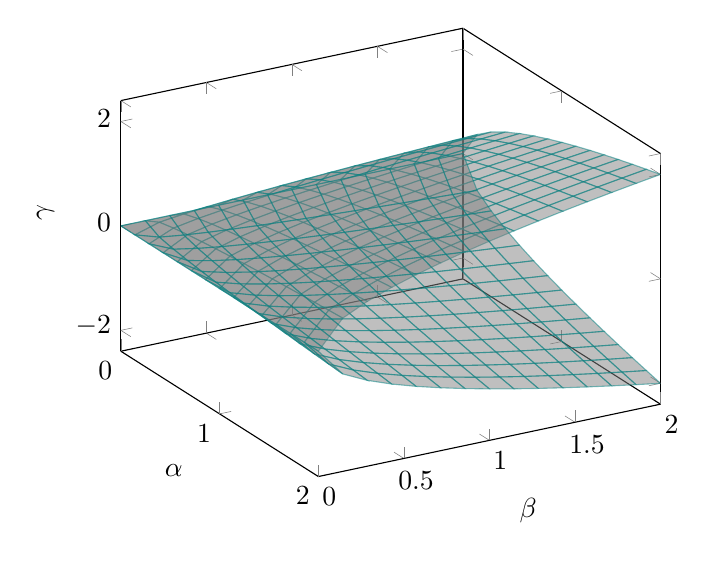
\begin{tikzpicture}
\begin{axis}[
  view={60}{30},
    xlabel=$\alpha$,
    ylabel=$\beta$,
    zlabel=$\gamma$,
]
    \addplot3 [
        surf,
        color=gray,
        faceted color = teal,
        opacity=0.5,
        samples=15,
        domain=0:2,y domain=0:2
    ] {sqrt(x*y)};
    \addplot3 [
        surf,
        color=gray,
        opacity=0.5,
        color=gray,
        faceted color = teal,
        samples=15,
        domain=0:2,y domain=0:2
    ] {-sqrt(x*y)};
\end{axis}
\end{tikzpicture}

  \end{center}
  \caption{Illustration du cône SPD pour une matrice $2\times 2$. L'ensemble des matrices de covariance vis à l'intérieur ou sur le bord du cône représenté. On peut effectuer une visualisation similaire en utilisant le code à l'adresse: \url{https://github.com/AmmarMian/simulations_hdr/blob/main/1-context/cone_spd/main.py}.}\label{fig:context-figure-spdcone}
  \end{figure}

Une caractérisation géométrique de cet espace sera développé dans la \cref{ch:context-riemann} d'où nous tirerons des outils prenant en compte la structure intrinsèque de cet espace. \\

% TODO: Regarder si d'autres propriétés sont intéressantes à ce stade

On peut également citer les propriétés suivantes, qui sont utiles pour les démonstrations de propriétés statistiques :

\begin{property}[{Lien à la moyenne}]
  \label{prop:context-definition-linkmoy}
  On a la relation suivante avec la moyenne:
  \begin{equation}
    \MCov_\Variable = \E_\Variable\left\{ \Variable\Variable^\T \right\} - \Vmoy_\Variable\Vmoy_\Variable^\T.
    \label{eq:context-definition-linkmoy}
  \end{equation}

\end{property}

\begin{property}[{Transformation linéaire}]
  \label{prop:context-definition-lineartraonsformation}
  Soit un opérateur linéaire $\mat{A}\in\R^{\Nvar\times p}$, et la variable aléatoire $\Variablebis=\mat{A}\Variable$, on a alors:
  \begin{equation}
    \MCov_\Variablebis = \mat{A}\MCov_\Variable\mat{A}^\T \in \R^{pp}.
    \label{eq:context-definition-lineartraonsformation}
  \end{equation}

\end{property}

Cette dernière propriété est notemment utile quand il s'agit de montrer comme on le verra dans le \cref{ch:robust-detection}, des invariances de tests statistiques vis-à-vis des paramètres du problème. En outre, la matrice de covariance étant une matrice SPD, on a la propriété suivante:

\begin{property}[{Diagonalisation}]
  \label{prop:context-definition-diagonalisation}
  Puisque $\MCov_\Variable$ est symmétrique réelle, alors en vertu du théorème spectral, il existe un opérateur orthogonal $\Orth\in\R^{\Nvar\Nvar}$, i.e $\Orth=\Orth^\T$ et $\Orth^{-1}=\Orth^\T$, tel que :
  \begin{equation}
    \Orth\MCov_\Variable\Orth^\T = \Diag(\eig_1\dots,\eig_\Nvar),
    \label{eq:context-definition-diagonalisation}
  \end{equation}
  où $\Diag$ est l'opérateur qui construit une matrice diagonale à partir des éléments en argument et $\{\eig_1,\dots\eig_\Nvar\}$ sont les valeurs propres de $\MCov_\Variable$.

\end{property}

\section{Estimation}
\label{sec:context-covariance-estimation}

Une fois le cadre posé, un problème naturel qui émerge est l'estimation de la matrice de covariance étant donné un ensemble de données observées. Il s'agit alors à partir de mesures/observations d'estimer les tendances des variables présentes en termes de corrélations\footnote{On s'intéresse dans ce paragraphe à l'estimation sans à priori sur la loi de probabilités sous-jacente. Si l'on connait la loi à priori des données, on peut proposer le cadre de l'estimation au sens du maximum de vraisemblance comme ce sera fait en \cref{ch:context-distributions}.}.

Supposons une variable aléatoire multivariée $\Variable=[\variable_1,\dots,\variable_\Nvar]^\T$. Il est usuel d'observer ces variables sur un ensemble d'individus, ce qui nous amène à traiter un ensemble de données que l'on dénote $\Xset = \{\x_\iobs:1\leq\iobs\leq\Nobs\}$ ou bien sous forme de matrice :
\begin{equation}
  \X = \left[\x_1,\, \dots,\, \x_\Nobs \right]^\T = \left[ \begin{array}{ccc} x_{11} & \dots & x_{1\Nvar} \\ \vdots & \ddots & \vdots \\ x_{\Nvar 1} & \dots & x_{\Nvar \Nobs}   \end{array}  \right]\in\R^{\Nvar\Nobs}.
  \label{eq:context-definition-observed_data}
\end{equation}

On suppose également que ces observations sont i.i.d. Pour pouvoir calculer la covariance, il est d'abord nécessaire de s'intéresser à la moyenne:
\begin{proposition}[{Estimation de la moyenne d'un vecteur aléatoire}]
  \'Etant donné un ensemble d'observations $\X$ de la variable $\Variable$, un estimateur consistant et non-biaisé\footnote{Soit $\hat{\param}=f(\Variable)$ un estimateur d'une quantité $\param$ découlant de la variable $\Variable$. On dit que $\hat{\param}$ est \textbf{non-biaisé} si $\E_\Variable\{\hat{\param}\} = \param$. De même, on dit que l'estimateur est \textbf{consistant} si $\forall \epsilon>0,\, \displaystyle\lim_{\Nobs\to\infty} \Prob\left(|\hat{\param}-\param|>\epsilon\right)=0$.\\En d 'autres termes un estimateur non-biaisé est en moyenne autour de la vraie valeur cherchée et un estimateur consistant converge vers la vraie valeur avec suffisamment d'observations.} de la moyenne est:
  \begin{equation}
    \hat{\Vmoy}_\Variable = \frac{1}{\Nobs}\sum_{\iobs=1}^{\Nobs} \x_\iobs.
    \label{eq:context-estimation-moyenne}
  \end{equation}
\end{proposition}

\begin{remark}
  Il est facile de montrer, en vertu de la loi des grands nombres que pour $\Nobs\to\infty$:
  $$
  \hat{\Vmoy}_\Variable \approx \E_\Variable\{\Variable\}=\Vmoy_\Variable.
  $$
\end{remark}


\begin{remark}
  On peut retrouver le côté non-biaisé en prenant l'espérance de l'estimateur\footnote{On se permettra à partir de maintenant d'utiliser par simplification l'opérateur espérance sur les valeurs observées des variables sans aller chercher la variable aléatoire sous-jacente. On comprends que l'on regarde l'espérance d'une fonction des variables aléatoires et non de valeurs précises observées.}:
  $$
  \E_\Variable\left\{\hat{\Vmoy}_\Variable\right\} = \E_\Variable\left\{\frac{1}{\Nobs}\sum_{\iobs=1}^{\Nobs}\x_\iobs\right\} = \Vmoy_\Variable.
  $$
\end{remark}


Afin d'estimer la matrice de covariance, on peut en partant de cette première estimation avoir l'estimateur suivant:

\begin{proposition}[{Estimateur de la matrice de covariance}]
  \'Etant donné un ensemble d'observations $\X$ de la variable $\Variable$, un estimateur consistant et non-biaisé de la matrice de covariance est la scm:
  \begin{equation}
    \hat{\MCov}_\Variable =  \frac{1}{\Nobs-1}\sum_{\iobs=1}^{\Nobs} \left(\x_\iobs-\hat{\Vmoy}_x\right)\left(\x_\iobs-\hat{\Vmoy}_x\right)^\T.
    \label{eq:context-estimation-covariance}
  \end{equation}
\end{proposition}


\begin{remark}[{Caractère non-biaisé}]
  On remarque que le coefficient $(N-1)$ et non $N$ dans la fraction. Cela permet à notre estimateur d'être non biaisé. en effet, on peut montrer que:
$$
  E_\Variable\left\{\left(\x_\iobs-\hat{\Vmoy}_\Variable\right)\left(\x_\iobs-\hat{\Vmoy}_\Variable\right)^\T\right\} = \frac{N-1}{N}\MCov_\Variable.
$$
Il est ainsi nécessaire de compenser par le facteur $\frac{N}{N-1}$ pour obtenir un estimateur non-biaisé:


%  \vspace{-2em}
%   \begin{proof}
%   En effet, calculons l'espérance de celui-ci:
%   \begin{align*}
%     \E_\Variable\left\{ \hat{\MCov}_\Variable \right \} & =  \frac{1}{\Nobs-1}\sum_{\iobs=1}^{\Nobs} \E_\Variable\left\{\left(\x_\iobs-\hat{\Vmoy}_x\right)\left(\x_\iobs-\hat{\Vmoy}_x\right)^\T\right\}.
%   \end{align*}
%
% Développons l'expression à l'intérieur de l'espérance :
%   \begin{align*}
%     \left(\x_\iobs-\hat{\Vmoy}_\Variable\right)\left(\x_\iobs-\hat{\Vmoy}_\Variable\right)^\T &= \x_\iobs\x_\iobs^\T - \x_\iobs\hat{\Vmoy}_\Variable^\T - \hat{\Vmoy}_\Variable\x_\iobs^\T + \hat{\Vmoy}_\Variable\hat{\Vmoy}_\Variable^\T.
%   \end{align*}
%
%   En prenant l'espérance terme par terme et en utilisant le fait que les observations sont i.i.d :
%
%     \textbf{Terme 1 :} $\E_\Variable\left\{\x_\iobs\x_\iobs^\T\right\} = \MCov_\Variable + \Vmoy_\Variable\Vmoy_\Variable^\T$ en vertu de la \cref{prop:context-definition-linkmoy}.
%
%   \textbf{Terme 2 :} Sachant que $\hat{\Vmoy}_\Variable = \frac{1}{\Nobs}\sum_{j=1}^{\Nobs} \x_j$ :
%   \begin{align*}
%     \E_\Variable\left\{\x_\iobs\hat{\Vmoy}_\Variable^\T\right\} &= \E_\Variable\left\{\x_\iobs \cdot \frac{1}{\Nobs}\sum_{j=1}^{\Nobs} \x_j^\T\right\} = \frac{1}{\Nobs}\sum_{j=1}^{\Nobs} \E_\Variable\left\{\x_\iobs\x_j^\T\right\}
%   \end{align*}
%
%   Comme les observations sont i.i.d :
%   \begin{itemize}
%     \item Si $\iobs = j$ : $\E_\Variable\left\{\x_\iobs\x_j^\T\right\} = \MCov_\Variable + \Vmoy_\Variable\Vmoy_\Variable^\T$
%     \item Si $\iobs \neq j$ : $\E_\Variable\left\{\x_\iobs\x_j^\T\right\} = \Vmoy_\Variable\Vmoy_\Variable^\T$
%   \end{itemize}
%
%   \begin{align*}
%     \text{Donc :} \E_\Variable\left\{\x_\iobs\hat{\Vmoy}_\Variable^\T\right\} &= \frac{1}{\Nobs}\left[(\MCov_\Variable + \Vmoy_\Variable\Vmoy_\Variable^\T) + (\Nobs-1)\Vmoy_\Variable\Vmoy_\Variable^\T\right] = \frac{1}{\Nobs}\MCov_\Variable + \Vmoy_\Variable\Vmoy_\Variable^\T
%   \end{align*}
%
%   \textbf{Terme 3 :} Par symétrie : $\E_\Variable\left\{\hat{\Vmoy}_\Variable\x_\iobs^\T\right\} = \frac{1}{\Nobs}\MCov_\Variable + \Vmoy_\Variable\Vmoy_\Variable^\T$
%
%
%   \begin{align*}
%     \text{\bfseries Terme 4 :} \E_\Variable\left\{\hat{\Vmoy}_\Variable\hat{\Vmoy}_\Variable^\T\right\} &= \E_\Variable\left\{\frac{1}{\Nobs^2}\sum_{j=1}^{\Nobs}\sum_{\iobs=1}^{\Nobs} \x_j\x_\iobs^\T\right\} = \frac{1}{\Nobs^2}\sum_{j=1}^{\Nobs}\sum_{\iobs=1}^{\Nobs} \E_\Variable\left\{\x_j\x_\iobs^\T\right\}
%   \end{align*}
%
%   Il y a $\Nobs$ termes avec $j = \iobs$ et $\Nobs^2 - \Nobs$ termes avec $j \neq \iobs$, d'où :
%   \begin{align*}
%     \E_\Variable\left\{\hat{\Vmoy}_\Variable\hat{\Vmoy}_\Variable^\T\right\} &= \frac{1}{\Nobs^2}\left[\Nobs(\MCov_\Variable + \Vmoy_\Variable\Vmoy_\Variable^\T) + (\Nobs^2-\Nobs)\Vmoy_\Variable\Vmoy_\Variable^\T\right] = \frac{1}{\Nobs}\MCov_\Variable + \Vmoy_\Variable\Vmoy_\Variable^\T
%   \end{align*}
%
%   \begin{align*}
%     \text{Donc} &\E_\Variable\left\{\left(\x_\iobs-\hat{\Vmoy}_\Variable\right)\left(\x_\iobs-\hat{\Vmoy}_\Variable\right)^\T\right\} \\
%     &= (\MCov_\Variable + \Vmoy_\Variable\Vmoy_\Variable^\T) - 2\left(\frac{1}{\Nobs}\MCov_\Variable + \Vmoy_\Variable\Vmoy_\Variable^\T\right) + \left(\frac{1}{\Nobs}\MCov_\Variable + \Vmoy_\Variable\Vmoy_\Variable^\T\right) \\
%     &= \MCov_\Variable - \frac{1}{\Nobs}\MCov_\Variable = \frac{\Nobs-1}{\Nobs}\MCov_\Variable\\
%     \text{Conclusion :} & \E_\Variable\left\{ \hat{\MCov}_\Variable \right \} = \frac{1}{\Nobs-1}\sum_{\iobs=1}^{\Nobs} \frac{\Nobs-1}{\Nobs}\MCov_\Variable \\
%     &= \frac{1}{\Nobs-1} \cdot \Nobs \cdot \frac{\Nobs-1}{\Nobs}\MCov_\Variable = \MCov_\Variable.
%   \end{align*}
%
%   L'estimateur est donc bien non-biaisé, ce qui justifie l'utilisation du coefficient $\frac{1}{\Nobs-1}$ plutôt que $\frac{1}{\Nobs}$.
% \end{proof}
\end{remark}


\begin{remark}
Une fois que l'on connait $E_\Variable\left\{\left(\x_\iobs-\hat{\Vmoy}_\Variable\right)\left(\x_\iobs-\hat{\Vmoy}_\Variable\right)^\T\right\}$, on peut utiliser la loi des grands nombres pour dire que lorsque $\Nobs\to\infty$\footnote{il ne s'agit pas d'une démonstration de la consistance théorique, qui requiert des conditions de régularité sur la d.d.p sous-jacente mais cela illustre un comportement en ce sens.}:
  \begin{align*}
    \hat{\MCov}_\Variable &= \frac{\Nobs}{\Nobs-1}\times\frac{1}{\Nobs} \sum_{\iobs=1}^\Nobs\left(\x_\iobs-\hat{\Vmoy}_\Variable\right)\left(\x_\iobs-\hat{\Vmoy}_\Variable\right)^\T \\
    & \approx  \frac{\Nobs}{\Nobs-1} E_\Variable\left\{\left(\x_\iobs-\hat{\Vmoy}_\Variable\right)\left(\x_\iobs-\hat{\Vmoy}_\Variable\right)^\T\right\}  = \MCov_\Variable.
\end{align*}
\end{remark}


Il est intéressant de regarder à travers une simulation numérique, la convergence de nos deux estimateurs dans le régime $\Nobs\to\infty$. Pour ce faire, nous simulons des données de moyenne $\Vmoy_\Variable = [1,\dots,1]^\T$ et de matrice de covariance $\MCov_\Variable=\Id{\Nvar}$ en générant des données gaussiennes de moyenne $1$ et variance $1$ pour chaque observation $x_{\ivar\iobs}$. On représente alors en \cref{fig:context-estimation-errorscm}, l'erreur d'estimation\footnote{On utilise pour cela la norme euclidienne d'ordre 2 mais nous verrons dans la \cref{ch:context-riemann} que ce choix peut être discuté.} en fonction du nombre d'observations $\Nobs$. Même si ces simulations ne suffisent pas à elles seules à montrer la consistance et la convergence de nos estimateurs aux vraies paramètres de nos variables aléatoires, on peut observer à la fois une baisse de l'erreur en moyenne mais également que la variance de l'erreur diminue. On caractérisera ces deux comportements en \cref{ch:context-distributions} dans un cadre où l'on ajoute un à priori sur la distribution sous-jacente des données.
% TODO: ne pas oublier de faire consistance avec à-priori gaussien et elliptique si possible.

\begin{figure*}[h]
    \begin{center}
    % This file was created with matplot2tikz v0.5.3.
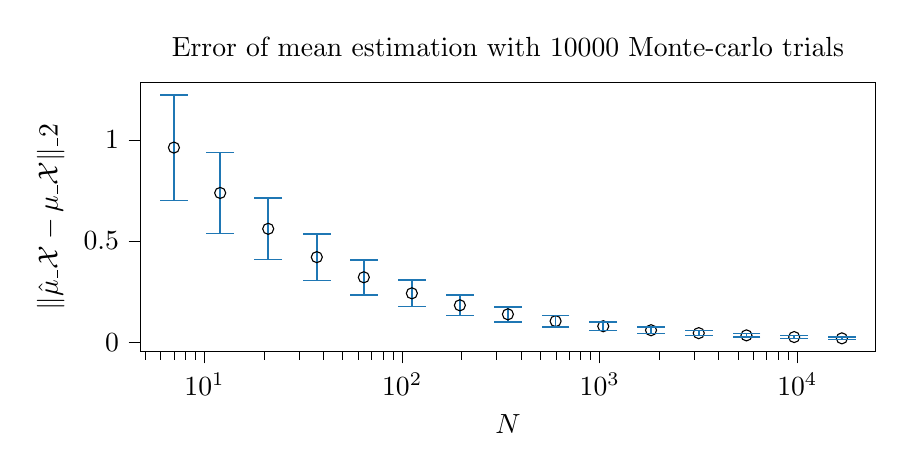
\begin{tikzpicture}

\definecolor{darkgray176}{RGB}{176,176,176}
\definecolor{steelblue31119180}{RGB}{31,119,180}

\begin{axis}[
width=0.9\textwidth,
height=5cm,
log basis x={10},
tick align=outside,
tick pos=left,
title={Error of mean estimation with 10000 Monte-carlo trials},
x grid style={darkgray176},
xlabel={\(\displaystyle N\)},
xmin=4.74327639380337, xmax=24803.3195269196,
xmode=log,
xtick style={color=black},
y grid style={darkgray176},
ylabel={\(\displaystyle \|\hat{\boldsymbol{\mu}}\_\mathcal{X} - \boldsymbol{\mu}\_\mathcal{X}\|\_2\)},
ymin=-0.0461003164651899, ymax=1.28319327993008,
ytick style={color=black}
]
\addplot [draw=black, mark=o, only marks]
table{%
x  y
7 0.961809938446161
12 0.737728543463078
21 0.560616951169621
37 0.420661897373797
64 0.32120978405099
112 0.242018240638433
196 0.182805838986852
343 0.138405338128785
598 0.104765688177838
1042 0.0794917535174116
1818 0.0598006596884444
3170 0.0453866342512824
5528 0.0343647504602777
9639 0.026099922904704
16807 0.0196559171311048
};
\path [draw=steelblue31119180, semithick]
(axis cs:7,0.700849033162032)
--(axis cs:7,1.22277084373029);

\path [draw=steelblue31119180, semithick]
(axis cs:12,0.537975705847932)
--(axis cs:12,0.937481381078224);

\path [draw=steelblue31119180, semithick]
(axis cs:21,0.409881143046451)
--(axis cs:21,0.711352759292791);

\path [draw=steelblue31119180, semithick]
(axis cs:37,0.306090426059901)
--(axis cs:37,0.535233368687693);

\path [draw=steelblue31119180, semithick]
(axis cs:64,0.234693244705277)
--(axis cs:64,0.407726323396703);

\path [draw=steelblue31119180, semithick]
(axis cs:112,0.176615269618465)
--(axis cs:112,0.307421211658401);

\path [draw=steelblue31119180, semithick]
(axis cs:196,0.133295627068537)
--(axis cs:196,0.232316050905168);

\path [draw=steelblue31119180, semithick]
(axis cs:343,0.101071846947206)
--(axis cs:343,0.175738829310364);

\path [draw=steelblue31119180, semithick]
(axis cs:598,0.0764314707238397)
--(axis cs:598,0.133099905631837);

\path [draw=steelblue31119180, semithick]
(axis cs:1042,0.0578812731877006)
--(axis cs:1042,0.101102233847123);

\path [draw=steelblue31119180, semithick]
(axis cs:1818,0.0435629040530663)
--(axis cs:1818,0.0760384153238226);

\path [draw=steelblue31119180, semithick]
(axis cs:3170,0.0331333015828912)
--(axis cs:3170,0.0576399669196737);

\path [draw=steelblue31119180, semithick]
(axis cs:5528,0.0251640440466649)
--(axis cs:5528,0.0435654568738906);

\path [draw=steelblue31119180, semithick]
(axis cs:9639,0.0190071644585281)
--(axis cs:9639,0.0331926813508799);

\path [draw=steelblue31119180, semithick]
(axis cs:16807,0.0143221197345949)
--(axis cs:16807,0.0249897145276147);

\addplot [semithick, steelblue31119180, mark=-, mark size=5, mark options={solid}, only marks]
table {%
7 0.700849033162032
12 0.537975705847932
21 0.409881143046451
37 0.306090426059901
64 0.234693244705277
112 0.176615269618465
196 0.133295627068537
343 0.101071846947206
598 0.0764314707238397
1042 0.0578812731877006
1818 0.0435629040530663
3170 0.0331333015828912
5528 0.0251640440466649
9639 0.0190071644585281
16807 0.0143221197345949
};
\addplot [semithick, steelblue31119180, mark=-, mark size=5, mark options={solid}, only marks]
table {%
7 1.22277084373029
12 0.937481381078224
21 0.711352759292791
37 0.535233368687693
64 0.407726323396703
112 0.307421211658401
196 0.232316050905168
343 0.175738829310364
598 0.133099905631837
1042 0.101102233847123
1818 0.0760384153238226
3170 0.0576399669196737
5528 0.0435654568738906
9639 0.0331926813508799
16807 0.0249897145276147
};
\end{axis}

\end{tikzpicture}

    % This file was created with matplot2tikz v0.5.3.
\begin{tikzpicture}

\definecolor{darkgray176}{RGB}{176,176,176}
\definecolor{steelblue31119180}{RGB}{31,119,180}

\begin{axis}[
width=0.9\textwidth,
height=5cm,
log basis x={10},
tick align=outside,
tick pos=left,
x grid style={darkgray176},
xlabel={\(\displaystyle N\)},
xmin=4.74327639380337, xmax=24803.3195269196,
xmode=log,
xtick style={color=black},
y grid style={darkgray176},
ylabel={\(\displaystyle \|\hat{\MCov}_\Variable - \MCov_\Variable \|_2\)},
ymin=-0.13262423207483, ymax=3.87655604361312,
ytick style={color=black}
]
\addplot [draw=black, mark=o, only marks]
table{%
x  y
7 2.96644841886547
12 2.21671185618484
21 1.64709208228737
37 1.23397594189885
64 0.935112170973186
112 0.703404726719878
196 0.531310446912574
343 0.400325303184381
598 0.303923396605062
1042 0.230114283599226
1818 0.174038501677559
3170 0.131597391353147
5528 0.0998109498844136
9639 0.0753512175742832
16807 0.0572766951577409
};
\path [draw=steelblue31119180, semithick]
(axis cs:7,2.23857626119455)
--(axis cs:7,3.69432057653639);

\path [draw=steelblue31119180, semithick]
(axis cs:12,1.76497915252549)
--(axis cs:12,2.6684445598442);

\path [draw=steelblue31119180, semithick]
(axis cs:21,1.35747786948254)
--(axis cs:21,1.9367062950922);

\path [draw=steelblue31119180, semithick]
(axis cs:37,1.0374123409997)
--(axis cs:37,1.43053954279801);

\path [draw=steelblue31119180, semithick]
(axis cs:64,0.795915368703914)
--(axis cs:64,1.07430897324246);

\path [draw=steelblue31119180, semithick]
(axis cs:112,0.603021809771917)
--(axis cs:112,0.803787643667839);

\path [draw=steelblue31119180, semithick]
(axis cs:196,0.458345285906057)
--(axis cs:196,0.604275607919091);

\path [draw=steelblue31119180, semithick]
(axis cs:343,0.345034478896582)
--(axis cs:343,0.455616127472181);

\path [draw=steelblue31119180, semithick]
(axis cs:598,0.262460291581848)
--(axis cs:598,0.345386501628276);

\path [draw=steelblue31119180, semithick]
(axis cs:1042,0.198925436760575)
--(axis cs:1042,0.261303130437877);

\path [draw=steelblue31119180, semithick]
(axis cs:1818,0.150584064767169)
--(axis cs:1818,0.197492938587949);

\path [draw=steelblue31119180, semithick]
(axis cs:3170,0.114065796158437)
--(axis cs:3170,0.149128986547856);

\path [draw=steelblue31119180, semithick]
(axis cs:5528,0.0865643002479931)
--(axis cs:5528,0.113057599520834);

\path [draw=steelblue31119180, semithick]
(axis cs:9639,0.0652154542494471)
--(axis cs:9639,0.0854869808991193);

\path [draw=steelblue31119180, semithick]
(axis cs:16807,0.0496112350018946)
--(axis cs:16807,0.0649421553135873);

\addplot [semithick, steelblue31119180, mark=-, mark size=5, mark options={solid}, only marks]
table {%
7 2.23857626119455
12 1.76497915252549
21 1.35747786948254
37 1.0374123409997
64 0.795915368703914
112 0.603021809771917
196 0.458345285906057
343 0.345034478896582
598 0.262460291581848
1042 0.198925436760575
1818 0.150584064767169
3170 0.114065796158437
5528 0.0865643002479931
9639 0.0652154542494471
16807 0.0496112350018946
};
\addplot [semithick, steelblue31119180, mark=-, mark size=5, mark options={solid}, only marks]
table {%
7 3.69432057653639
12 2.6684445598442
21 1.9367062950922
37 1.43053954279801
64 1.07430897324246
112 0.803787643667839
196 0.604275607919091
343 0.455616127472181
598 0.345386501628276
1042 0.261303130437877
1818 0.197492938587949
3170 0.149128986547856
5528 0.113057599520834
9639 0.0854869808991193
16807 0.0649421553135873
};
\end{axis}

\end{tikzpicture}

  \end{center}
  \provScmmeanQR[.5cm]
    \caption{\'Evolution de l'erreur d'estimation de la moyenne et de la matrice de covariance en fonction de $\Nobs$ pour $\Nvar=7$. Les marqueurs correspondent à la moyenne de l'erreur d'estimation et les barres correspondent à la déviation standard de cette même erreur. Le nombre de tirages de monte-carlo est de $ 10^4$. \provScmcov}
  \label{fig:context-estimation-errorscm}
\end{figure*}



\section{Estimation régularisée}
\label{sec:context-covariance-regularized-estimation}

  


L'estimateur classique de la matrice de covariance donné par \cref{eq:context-definition-covariance-formula} présente des limitations importantes dans certains régimes dimensionnels. En effet, lorsque le nombre de variables $\Nvar$ devient comparable ou supérieur au nombre d'observations $\Nobs$, cet estimateur souffre de plusieurs défauts majeurs qui compromettent sa fiabilité pratique.

Le premier problème concerne le rang de la matrice estimée. Dans le cas extrême où $\Nvar > \Nobs$, la matrice $\hat{\MCov}_\Variable$ est nécessairement singulière, car elle est construite comme une somme de $\Nobs$ matrices de rang 1. Plus précisément, son rang est au plus $\min(\Nvar, \Nobs-1)$\footnote{Le facteur $N-1$ plutôt que $N$ est dû au fait que l'on additionne des matrices construites à partir d'observations dont on a soustrait la moyenne et donc introduit une relation linéaire d'ordre 1.}, ce qui la rend non-inversible lorsque $\Nvar \geq \Nobs$. Cette singularité pose des difficultés majeures pour de nombreuses applications statistiques nécessitant l'inversion de la matrice de covariance, comme l'analyse discriminante ou certaines méthodes de classification. Au-delà de ce problème de rang, même dans le régime sous-déterminé où $\Nvar < \Nobs$ mais où le rapport $\Nvar/\Nobs$ n'est pas négligeable\footnote{Ce qui sera le cas dans de nombreuses approches basé sur une estimation de la covariance en apprentissage profond. Voir pour cela le \cref{ch:spdnet}.}, l'estimateur empirique souffre d'une grande variabilité. Cette variabilité se manifeste notamment par une dispersion importante des valeurs propres de $\hat{\MCov}_\Variable$ autour de celles de la vraie matrice $\MCov_\Variable$. Cela peut être analysé au travers de la notion de conditionnement:

\begin{figure}
  \begin{center}
      \begin{minipage}{0.45\textwidth}
        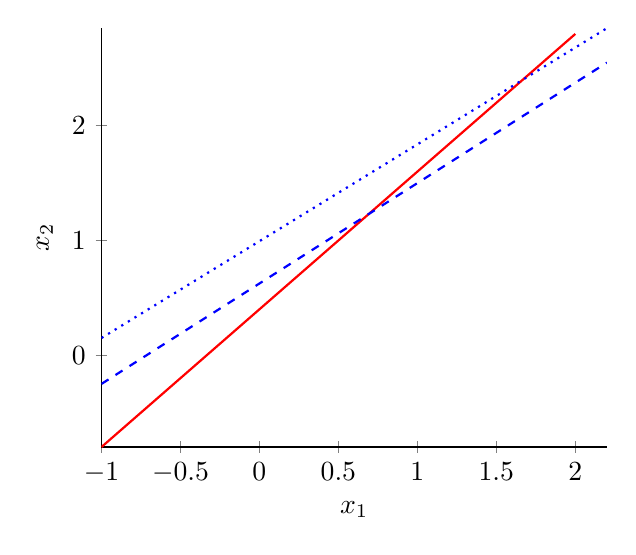
\begin{tikzpicture}
\begin{axis}[
    width=8cm,
    xlabel={$x_1$},
    ylabel={$x_2$},
    axis lines=left,
    axis line style={-},
]
\addplot[red, thick] coordinates {(-1, -0.8) (2, 2.8)};
\addplot[blue, thick, dashed] coordinates {(-1, -0.25) (2.2, 2.55)};
\addplot[blue, thick, dotted] coordinates {(-1, 0.15) (2.2, 2.85)};
\end{axis}
\end{tikzpicture}

      \end{minipage}
      \begin{minipage}{0.45\textwidth}
        
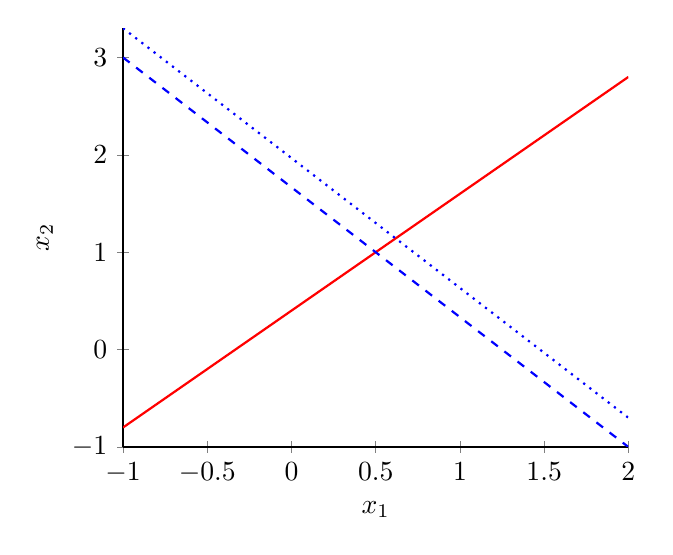
\begin{tikzpicture}
\begin{axis}[
    width=8cm,
    xlabel={$x_1$},
    ylabel={$x_2$},
    axis lines=left,
    axis line style={-},
]
\addplot[red, thick] coordinates {(-1, -0.8) (2, 2.8)};
  \addplot[blue, thick, dashed] coordinates {(-1, 3) (2, -1)};
  \addplot[blue, thick, dotted] coordinates {(-1, 3.3) (2, -0.7)};
\end{axis}
\end{tikzpicture}

      \end{minipage}
      \vspace{-2em}
      \end{center}
  \caption{Illustration visuelle du conditionnement d'un système linéaire dans le cas où $\mat{A}\in\R^{2\times 2}$. La solution correspond à l'intersection des droites continues (-) et en pointillés (- -). Une perturbation sur $\vector{b}$ déplace la droite (- -) en (..). À gauche: le cas d'une matrice mal conditionnée car la solution bouge beaucoup à cause de la perturbation. À droite: la perturbation a moins d'effet sur la solution.}\label{fig:context-estimation-condition}
\end{figure}

  \begin{definition}[{Conditionnement d'une matrice à l'inversion}]
    Le conditionnement d'une matrice $\mat{A}\in\R^{pq}$  est donné par :
    \begin{equation}
      \Cond(\mat{A}) = \|\mat{A}\|_2\|\mat{A}^{-1}\|_2.
      \label{eq:context-estimation-condition}
    \end{equation}
    
  \end{definition}

  \begin{remark}
Il correspond à un nombre quantifiant la sensibilité de la solution au système linéaire:
$$
    \mat{A}\x = \vector{b},
$$
    où $\x\in\R^q$ est la solution cherchée et $\vector{b}\in\R^q$ est un vecteur de constantes. En effet, supposant une erreur d'approximation $\vector{e}\in\R^q$ sur le vecteur $\vector{b}$, résoudre en pratique le système :
  $$
      \mat{A}\x = \vector{b}+\vector{e},
  $$
    provoque une erreur sur la solution de l'ordre $\mat{A}^{-1}\vector{e}$. En quantifiant le ratio entre l'erreur relative sur la solution et sur $\vector{b}$ :
    $$
     \epsilon(\vector{e}) =  \left. \frac{\|\mat{A}^{-1}\vector{e}\|_2}{\| \mat{A}^{-1}\vector{b}\|_2} \displaystyle \middle/ \frac{\|\vector{e}\|_2}{\| \vector{b}\|_2} \right. ,
    $$

    on a pour $\vector{e}\neq \vector{0}$ et $\vector{b}\neq\vector{0}$, $\max_{\vector{e}}\epsilon(\vector{e})=\Cond(\mat{A})$.

    Ainsi, ce nombre nous donne une information sur la praticabilité d'une matrice obtenue par estimation vis à vis de problèmes nécessitant son inversion. Ce principe est illustré en \cref{fig:context-estimation-condition}.
  \end{remark}

Notamment dans le cas de matrices carrée symétriques, on a le résultat suivant :

\begin{proposition}[{Conditionnement d'une matrice symmétrique}]
  Soit une matrice $\mat{A}\in\R^{\Nvar\Nvar}$ tel que $\mat{A}=\mat{A}^\T$, on peut calculer le conditionnement de cette matrice vis-à-vis de l'inversion donnée en \cref{eq:context-estimation-condition} avec:
    \begin{equation}
      \Cond(\mat{A}) = \frac{\max |\eigset(\mat{A})|}{\min |\eigset(\mat{A})|},
      \label{eq:context-estimation-conditionspd}
    \end{equation}
  où $\eigset(\mat{A})$ est l'ensemble des valeurs propres de $\mat{A}$.
\end{proposition}




Si l'on revient à l'estimation de notre matrice de covariance, on peut quantifier la dispersion en pratique : en simulant des données aléatoires de la même façon que précédemment en \cref{sec:context-covariance-estimation} avec une moyenne et matrice covariance connues. Plutôt que de regarder l'erreur d'estimation, on s'intéresse au conditionnement de la matrice estimée en \cref{fig:context-estimation-cond}. On s'aperçoit alors que dés que la taille de la matrice approche ou dépasse le nombre d'observations, le conditionnement de la matrice explose, i.e, les valeurs propres ont une très grande dispersion, ce qui est problématique pour un certain nombre d'applications dépendant d'une SVD de cette matrice, tel que l'analyse en composantes principales par exemple. \\

\begin{figure}[h]
  \begin{center}
        % This file was created with matplot2tikz v0.5.3.
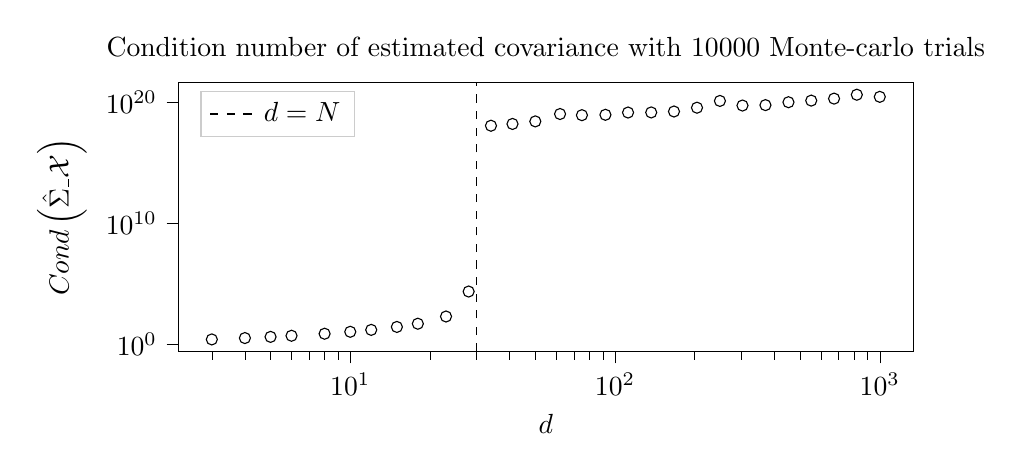
\begin{tikzpicture}

\definecolor{darkgray176}{RGB}{176,176,176}
\definecolor{lightgray204}{RGB}{204,204,204}

\begin{axis}[
width=0.9\textwidth,
height=5cm,
legend cell align={left},
legend style={
  fill opacity=0.8,
  draw opacity=1,
  text opacity=1,
  at={(0.03,0.97)},
  anchor=north west,
  draw=lightgray204
},
log basis x={10},
log basis y={10},
tick align=outside,
tick pos=left,
title={Condition number of estimated covariance with 10000 Monte-carlo trials},
x grid style={darkgray176},
xlabel={\(\displaystyle d\)},
xmin=2.2437647322819, xmax=1337.03857487278,
xmode=log,
xtick style={color=black},
y grid style={darkgray176},
ylabel={\(\displaystyle \operatorname{Cond}\left(\hat{\boldsymbol{\Sigma}}\_\mathcal{X}\right)\)},
ymin=0.22380594276999, ymax=4.1309909352877e+21,
ymode=log,
ytick style={color=black}
]
\addplot [draw=black, forget plot, mark=o, only marks]
table{%
x  y
3 2.30128721449648
4 2.98980176023402
5 3.74725148388153
6 4.6273062005471
8 6.80978228176998
10 9.85053405764688
12 14.1914261593259
15 24.8541084638651
18 45.8675117285121
23 181.624000745188
28 21118.5385109043
34 1.09423163871398e+18
41 1.54003337498655e+18
50 2.50285206785319e+18
62 1.02082277017018e+19
75 8.1696391406987e+18
92 8.78584488032868e+18
112 1.35351469825842e+19
137 1.37578020462997e+19
167 1.64652490481264e+19
204 3.4004576745693e+19
249 1.23230576162333e+20
303 5.12553978317069e+19
370 5.56209683272156e+19
452 9.65397291811529e+19
551 1.31245394055025e+20
672 1.91723632520982e+20
819 4.01749210190887e+20
1000 2.688261444791e+20
};
\addplot [semithick, black, dashed]
table {%
30 0.22380594276999
30 4.1309909352877e+21
};
\addlegendentry{$d=N$}
\end{axis}

\end{tikzpicture}

      \end{center}
  \provScmcondQR[.5cm]
  \caption{\'Evolution du conditionnement de la matrice estimée  par SCM pour une taille croissante de variables $\Nvar$ avec $\Nobs=30$. Les marqueurs indique la moyenne du conditionnement sur 50 tirages de monte-carlo. \provScmcond}
  \label{fig:context-estimation-cond}
\end{figure}



Pour pallier les défauts de l'estimateur empirique en haute dimension, \sidecite[0cm]{LedoitWolf2004} proposent un estimateur régularisé de la forme :

\begin{definition}[{Estimateur de Ledoit-Wolf}]
\begin{equation}
  \hat{\MCov}_\Variable^{\text{LW}}(\coefledoitwolf) = (1-\coefledoitwolf) \hat{\MCov}_\Variable + \coefledoitwolf \targetledoitwolf
\label{eq:context-ledoit-wolf}
\end{equation}
où $\coefledoitwolf \in [0,1]$ est un coefficient de régularisation et $\targetledoitwolf$ est une matrice cible (\textit{target}) de même dimension que $\hat{\MCov}_\Variable$.
\end{definition}

L'idée fondamentale de cette approche consiste à contracter l'estimateur empirique vers une matrice cible $\targetledoitwolf$ possédant de meilleures propriétés de conditionnement. Le choix le plus courant pour cette matrice cible est la matrice identité mise à l'échelle : $\targetledoitwolf = \frac{\Tr(\hat{\MCov}_\Variable)}{\Nvar} \mathbf{I}_\Nvar$. Cette cible correspond à l'hypothèse que toutes les variables ont la même variance (égale à la variance moyenne) et sont non corrélées entre elles. Ainsi, l'estimateur se veut être un compromis entre l'estimation SCM et une hypothèse de variables faiblement corrélées.

Le choix du coefficient $\coefledoitwolf$ est fait à priori mais si l'on définit un critère de eqm sur la qualité de l'estimation:
\begin{equation}
  \loss(\hat{\MCov}_\Variable(\coefledoitwolf), \MCov_\Variable) = \| \hat{\MCov}_\Variable(\coefledoitwolf) - \MCov_\Variable \|_\frob^2
  \label{eq:context-estimation-losslwf}
\end{equation}
sous le modèle donné en \cref{eq:context-ledoit-wolf}, on peut alors vouloir trouver l'optimal au sens statistique.
%TODO: Verify this loss, notably squared

Pour ce faire, nous nous intéressons à l'espérance du critère défini en \cref{eq:context-estimation-losslwf}:
$$
  \risk(\coefledoitwolf) = \E_\Variable\left\{\loss(\hat{\MCov}_\Variable(\coefledoitwolf), \MCov_\Variable)\right\},
$$

et l'on veut résoudre:
\begin{equation}
  \coefledoitwolf^\star = \arg\min_\coefledoitwolf \risk(\coefledoitwolf).
\end{equation}

%TODO : parler de l'estimation de alpha optimal dans la partie ddp

% On peut alors montrer en développant les termes de la norme et solvant $\frac{\partial\risk(\coefledoitwolf) }{\partial\coefledoitwolf}=0$ que la solution optimale est atteinte en:
%
% $$\coefledoitwolf^\opt = \frac{\E\left\{\|\hat{\MCov}_\Variable - \MCov_\Variable\|_\frob^2\right\} - \E\left\{\Tr\left((\hat{\MCov}_\Variable - \MCov_\Variable)(\targetledoitwolf - \MCov_\Variable)^T\right)\right\}}{\|\targetledoitwolf - \MCov_\Variable\|_\frob^2}$$
% %TODO: verify this
%
% En exprimant cette solution en termes des éléments matriciels individuels et en utilisant les propriétés d'espérance des estimateurs empiriques, cette expression se reformule sous la forme pratique suivante:
%
%
% \begin{proposition}[{Estimation optimale du coefficient de régularisation}]
% Le coefficient optimal $\coefledoitwolf^*$ au sens de la minimisation de l'erreur quadratique moyenne est donné par :
% \begin{equation}
% \coefledoitwolf^* = \frac{\sum_{i,j} \text{Var}(\hat{\sigma}_{ij})}{\sum_{i,j} (\hat{\sigma}_{ij} - t_{ij})^2}
% \label{eq:context-alpha-optimal}
% \end{equation}
% où $\hat{\sigma}_{ij}$ et $t_{ij}$ désignent respectivement les éléments $(i,j)$ des matrices $\hat{\MCov}_\Variable$ et $\targetledoitwolf$.
% \end{proposition}
%



\begin{figure}
  \begin{tikzpicture}
\begin{axis}[
    width=8cm,
    height=4cm,
    xlabel={$\coefledoitwolf$},
    ylabel={$\risk(\coefledoitwolf)$},
    xmin=0, xmax=1,
    ymin=0, ymax=3,
    grid=none,
    grid style={gray!30},
    legend style={
        fill=none,
        draw=none,
        at={(0,1.1)},
        anchor=south west,
    },
    legend cell align={left},
    % Custom axis labels
    xtick={0,1},
    ymajorticks=false,
    axis lines=left,
    axis line style={-},
]


% Variance curve - matches the dashed line in your figure
% Decreases from 1.8 to 1.2 with gentle quadratic curvature
\addplot[
    thick,
    dashed,
    domain=0.001:1,
    samples=100
] {.2-ln(.25+x)};
\addlegendentry{Variance}

% Squared Bias curve - matches the dotted line in your figure  
% Increases from 0.3 to 1.3 with accelerating quadratic growth
\addplot[
    thick,
    dotted,
    domain=0:1,
    samples=100
] {0.01 - 0.2*x + 2.4*x^2};
\addlegendentry{Bias$^2$}

% Mean Squared Error - matches the solid U-shaped curve in your figure
% Sum of variance and bias: (1.8-0.9x+0.3x²) + (0.3-0.7x+1.7x²) = 2.1-1.6x+2.0x²
% Minimum at x=0.4 with value 1.78
\addplot[
    thick,
    solid,
    domain=0:1,
    samples=100
] {3*(x-0.4)^2+1.1};
\addlegendentry{EQM}

% Key estimation points with geometric markers

% Sample covariance matrix (left endpoint, λ=0)
% Square symbol represents the unregularized estimator
\addplot[
    only marks,
    mark=square*,
    mark size=2pt,
    mark options={fill=black}
] coordinates {(0, 1.6)};

% Identity target matrix (right endpoint, λ=1) 
% Diamond symbol represents the fully shrunk estimator
\addplot[
    only marks,
    mark=diamond*,
    mark size=2pt,
    mark options={fill=black}
] coordinates {(1, 2.2)};

% Optimal Ledoit-Wolf estimator (minimum of MSE curve at λ=0.4)
% Circle symbol represents the optimal compromise
\addplot[
    only marks,
    mark=*,
    mark size=2pt,
    mark options={fill=black}
] coordinates {(0.4, 1.1)};

% Annotations for the key estimation points
% Using axis coordinates ensures precise positioning relative to data points
\node[above, anchor=south west] at (axis cs:0, 1.65) {\tiny$\hat{\MCov}_\Variable$};  % Sample covariance at λ=0
\node[above, anchor=south east] at (axis cs:1, 2) {\tiny$\frac{\Tr(\hat{\MCov}_\Variable)}{\Nvar}\Id{\Nvar}$};  % Identity target at λ=1  
\node[above,] at (axis cs:0.4, 1.15) {\tiny $\hat{\MCov}_\Variable^{LW}$};  % Optimal Ledoit-Wolf at λ=0.4


\end{axis}


\end{tikzpicture}

  \caption{biais-variance pour la régularisation de Ledoit-Wolf. La régularisation optimale balance la variance décroissante avec l'augmentation du biais introduit qui argument. Inspiré de (\cite{LedoitWolf2004}).}
  \label{fig:context-estimation-lwfbiasvar}

\end{figure}


L'estimation pratique de $\coefledoitwolf^*$ nécessite une connaissance de la d.d.p des variables aléatoires dû à l'opérateur espérance dans le critère à minimiser. Sous l'hypothèse de normalité multivariée des données, ces variances peuvent être exprimées analytiquement en fonction des moments empiriques d'ordre supérieur comme on le verra par la suite. Pour le moment, on considère la valeur $\coefledoitwolf$ comme un choix de l'utilisateur.

En introduisant cet estimateur, nous avons nécessairement biaisé notre estimation en vertu de la contraction vers une matrice cible $\targetledoitwolf$ fixée\footnote{Sauf si on a par chance pris la vraie matrice mais l'on conviendra que ce scénario est très rare en pratique.}. Mais en permettant ce conditionnement de baisser, nous avons réduit la variance de notre estimateur. Ainsi on peut interpréter $\coefledoitwolf$ comme une valeur qui contrebalance le biais et la variance de l'estimateur, ce qui est détaillé dans le travail initial (\cite{LedoitWolf2004}). Une Illustration de ce principe est donné en \cref{fig:context-estimation-lwfbiasvar}.




% TODO: references pour chaque matrice cible.
\begin{remark}[{Variants de régularisation}]
Plusieurs variantes de l'lw ont été développées selon le choix de la matrice cible $\targetledoitwolf$. Outre la cible identité, on peut citer : (i) la cible diagonale $\targetledoitwolf = \text{diag}(\hat{\MCov}_\Variable)$ qui préserve les variances individuelles tout en annulant les corrélations, (ii) la cible à corrélation constante qui suppose une structure de corrélation équicorrélée, et (iii) des cibles adaptatives construites à partir de connaissances a priori sur la structure des données.
\end{remark}


L'estimateur de Ledoit-Wolf présente l'avantage théorique fondamental d'être toujours inversible dès lors que la matrice cible $\targetledoitwolf$ l'est, ce qui résout le problème de singularité inhérent à l'estimateur empirique en haute dimension. De plus, le choix optimal du coefficient $\coefledoitwolf^*$ garantit une réduction systématique de l'erreur quadratique moyenne par rapport à l'estimateur non régularisé, particulièrement prononcée dans les régimes où $\Nvar/\Nobs$ est élevé.

Regardons enfin, le même problème d'estimation qu'en \cref{fig:context-estimation-errorscm} en ajoutant l'estimateur régularisé avec un coefficient $\coefledoitwolf=0.1$. Les résultats présentés en \cref{fig:context-estimation-condlwf} montrent comment la matrice obtenue a un bien meilleur conditionnement\footnote{\'Evidemment, cela se fait au prix d'un biais de l'estimateur en pratique sauf dans le cas d'une covariance théorique égale à la matrice $\targetledoitwolf$.}.


\begin{figure}[h]
  \begin{center}
        % This file was created with matplot2tikz v0.5.3.
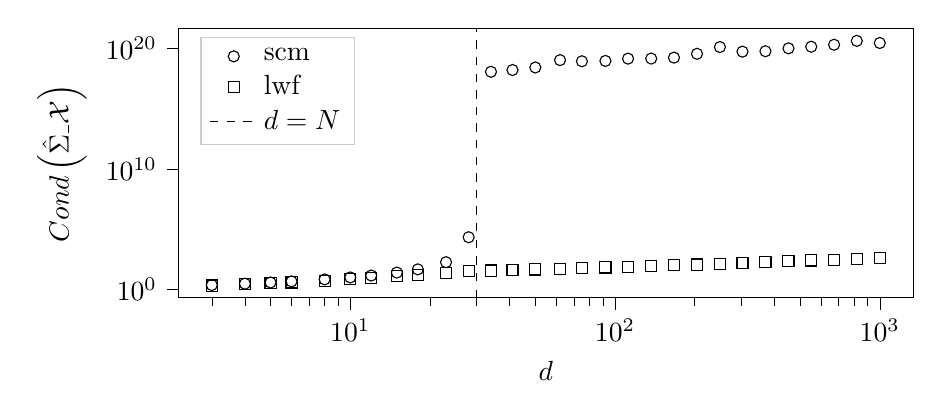
\begin{tikzpicture}

\definecolor{darkgray176}{RGB}{176,176,176}
\definecolor{lightgray204}{RGB}{204,204,204}

\begin{axis}[
width=0.9\textwidth,
height=5cm,
legend cell align={left},
legend style={
  fill opacity=0.8,
  draw opacity=1,
  text opacity=1,
  at={(0.03,0.97)},
  anchor=north west,
  draw=lightgray204
},
log basis x={10},
log basis y={10},
tick align=outside,
tick pos=left,
x grid style={darkgray176},
xlabel={\(\displaystyle d\)},
xmin=2.2437647322819, xmax=1337.03857487278,
xmode=log,
xtick style={color=black},
y grid style={darkgray176},
ylabel={\(\displaystyle \operatorname{Cond}\left(\hat{\boldsymbol{\Sigma}}\_\mathcal{X}\right)\)},
ymin=0.201647470461523, ymax=4.15155099642133e+21,
ymode=log,
ytick style={color=black}
]
\addplot [draw=black, mark=o, only marks]
table{%
x  y
3 2.30128721449648
4 2.98980176023402
5 3.74725148388153
6 4.6273062005471
8 6.80978228176998
10 9.85053405764688
12 14.1914261593259
15 24.8541084638651
18 45.8675117285121
23 181.624000745188
28 21118.5385109043
34 1.09423163871398e+18
41 1.54003337498655e+18
50 2.50285206785319e+18
62 1.02082277017018e+19
75 8.1696391406987e+18
92 8.78584488032868e+18
112 1.35351469825842e+19
137 1.37578020462997e+19
167 1.64652490481264e+19
204 3.4004576745693e+19
249 1.23230576162333e+20
303 5.12553978317069e+19
370 5.56209683272156e+19
452 9.65397291811529e+19
551 1.31245394055025e+20
672 1.91723632520982e+20
819 4.01749210190887e+20
1000 2.688261444791e+20
};
\addlegendentry{scm}
\addplot [draw=black, mark=square, only marks]
table{%
x  y
3 2.08376204777757
4 2.61314454230052
5 3.16591813272362
6 3.77123844164103
8 5.13511623080211
10 6.77168486719545
12 8.71032931589613
15 12.2362812865225
18 16.4991664311053
23 24.8178442526396
28 32.3101652848017
34 36.5636052780593
41 40.5410850707775
50 45.4758482161132
62 51.6716281093582
75 58.1312729983865
92 66.2939693288016
112 75.574506526652
137 86.8340390332717
167 99.9506811186795
204 115.670898107282
249 134.305665661733
303 156.108872096172
370 182.65218162239
452 214.359032952562
551 251.955200483623
672 297.023053266565
819 350.971958998932
1000 416.434315421376
};
\addlegendentry{lwf}
\addplot [semithick, black, dashed]
table {%
30 0.201647470461523
30 4.15155099642133e+21
};
\addlegendentry{$d=N$}
\end{axis}

\end{tikzpicture}

      \end{center}
  \provLwfcondQR[.5cm]
  \caption{\'Evolution du conditionnement de la matrice estimée par SCM et Ledoit-Wolf pour une taille croissante de variables $\Nvar$ avec $\Nobs=30$, $\coefledoitwolf=0.1$ et $\targetledoitwolf=\Id{\Nvar}$. Les marqueurs indique la moyenne du conditionnement sur 50 tirages de monte-carlo. \provLwfcond}
  \label{fig:context-estimation-condlwf}
\end{figure}



Nous nous sommes intéressés ici uniquement à la régularisation de Ledoit-Wolf car elle nous sera utile par la suite mais plusieurs approches alternatives existent. Pour un état de l'art sur le sujet, on peut se référer par exemple à \sidecite{Mohsen_Pourahmadi_2013}.


\section{Le cas complexe}
\label{sec:context-definition-complex}

Nous avons jusqu'ici supposé des observations réelles. Or dans beaucoup de cas, les données que l'on manipule sont complexes : c'est par exemple le cas dans le traitement de données issus d'une démodulation d'un signal en bande étroite comme cela peut être le cas dans le cadre de l'imagerie RSO\footnote{Radar à Synthèse d'ouverture} ou SONAR\footnote{Sound Navigation and Ranging} où le signal observé a une représentation complexe naturelle

Il serait tentant de considérer que tout ce qui précède se transpose mécaniquement en remplaçant les transpositions par des transpositions conjuguées. Mais c'est insuffisant: un vecteur aléatoire complexe n'est pas caractérisé au second ordre par sa seule matrice de covariance, il en faut une seconde, et l'usage universel de la première seule repose sur une hypothèse --- la circularité --- qu'il convient d'expliciter. Cette section met donc en place les objets d'ordre deux du cas complexe: la forme réelle, qui sera notre outil de démonstration systématique, puis le couple covariance--pseudo-covariance et la circularité. Le versant probabiliste --- constantes de normalisation, lois des formes quadratiques et jusqu'à la définition des fonctions de poids --- est traité en \cref{sec:context-distributions-complex}.

\subsection{Vecteurs aléatoires complexes et forme réelle}

Un vecteur aléatoire complexe $\Variable\in\C^\Nvar$ est un couple de vecteurs aléatoires réels, $\Variable = \Variable_x + j\Variable_y$ avec $\Variable_x,\Variable_y\in\R^\Nvar$. Sa loi \emph{est}, par définition, la loi conjointe du vecteur réel $2\Nvar$-dimensionnel obtenu par empilement, et il en va de même pour sa d.d.p. Tout ce que nous écrirons dans $\C^\Nvar$ peut donc être ramené à $\R^{2\Nvar}$, ce qui sera notre outil de démonstration systématique. Encore faut-il préciser ce que devient une matrice complexe dans cette correspondance :

\begin{definition}[{Forme réelle d'une matrice complexe}]
\label{def:context-complex-form}
  Soit $\mat{A}\in\C^{\Nvar\times\Nvar}$. On appelle \textbf{forme réelle} de $\mat{A}$ la matrice réelle $2\Nvar\times2\Nvar$
\begin{equation}
  \complexform{\mat{A}}
  \eqdef
  \begin{pmatrix}
    \Realp\mat{A} & -\Imagp\mat{A} \\
    \Imagp\mat{A} & \Realp\mat{A}
  \end{pmatrix}.
  \label{eq:context-complex-form}
\end{equation}
   En notant $\vector{v}=[\vector{x}^\T,\vector{y}^\T]^\T\in\R^{2\Nvar}$ le vecteur réel associé à $\vector{z}=\vector{x}+j\vector{y}$, on a l'équivalence $\mat{A}\vector{z} \longleftrightarrow \complexform{\mat{A}}\vector{v}$.
\end{definition}

De cette transformation complexe-réelle, on a naturellement les équivalences suivantes :

\begin{property}[{Transport des structures}]
\label{prop:context-complex-transport}
  L'application $\complexform{\cdot}$ est un morphisme injectif d'algèbres: $\complexform{\mat{A}\mat{B}} = \complexform{\mat{A}}\complexform{\mat{B}}$, $\complexform{\mat{A}+\mat{B}} = \complexform{\mat{A}}+\complexform{\mat{B}}$ et $\complexform{\inv{\mat{A}}} = \inv{\complexform{\mat{A}}}$. De plus:
  \begin{itemize}
    \item $\mat{A}$ est hermitienne si et seulement si $\complexform{\mat{A}}$ est symétrique;
    \item $\mat{A}$ est hermitienne définie positive si et seulement si $\complexform{\mat{A}}$ est symétrique définie positive, i.e, $\mat{A}\in\HPD{\Nvar}\iff\complexform{\mat{A}}\in\SPD{2\Nvar}$;
    \item $\mat{A}$ est unitaire si et seulement si $\complexform{\mat{A}}$ est orthogonale;
    \item $\Det(\complexform{\mat{A}}) = \abs{\Det(\mat{A})}^2$.
  \end{itemize}
\end{property}

  Cette correspondance est classique en analyse matricielle \sidecite[1.6cm]{hornjohnson2013matrix}, et son emploi en statistique complexe remonte au moins à \sidecite[-3cm]{Goodman1963}, qui dérive la d.d.p gaussienne complexe en passant par le vecteur réel de dimension $2\Nvar$. C'est en revanche sous la forme retenue ici, orientée estimation robuste, que la reprennent \cite{6263313}. Cet énoncé est l'outil central de toute la suite: chaque fois qu'un résultat du cas réel repose sur la seule structure du cône $\SPD{\cdot}$ — ce sera le cas des théorèmes d'existence et d'unicité que nous établirons en \cref{subsec:context-robust-m-estimation} — il se transporte au cas complexe sans nouvelle démonstration, en observant qu'une équation dans $\HPD{\Nvar}$ équivaut à la même équation dans $\SPD{2\Nvar}$ restreinte aux matrices de forme complexe.

  \begin{remark}
  Il donne aussi immédiatement le décompte des degrés de liberté, qui nous servira de fil conducteur. Une matrice de $\HPD{\Nvar}$ possède $\Nvar$ coefficients diagonaux réels et $\Nvar(\Nvar-1)/2$ coefficients extra-diagonaux complexes, soit $\Nvar^2$ paramètres réels libres, contre $\Nvar(\Nvar+1)/2$ dans le cas réel: il y a environ deux fois plus à estimer. Mais chaque observation apporte elle aussi deux fois plus de nombres réels, et nous verrons que ces deux facteurs se compensent exactement.
\end{remark}

\subsection{Statistiques d'ordre deux: covariance et pseudo-covariance}

Venons-en au point qui n'a pas d'équivalent réel. Dans $\R^\Nvar$, la matrice $\E\{\Variable\Variable^\T\}$ épuise l'information d'ordre deux. Dans $\C^\Nvar$, les moments d'ordre deux d'un vecteur centré sont au nombre de deux, selon que l'on conjugue ou non le second facteur.

\begin{definition}[{Covariance et pseudo-covariance}]
\label{def:context-complex-pseudocov}
  Soit $\Variable\in\C^\Nvar$ un vecteur aléatoire complexe centré de moments d'ordre deux finis. On appelle \textbf{matrice de covariance} et \textbf{matrice de pseudo-covariance}\footnote{Également appelée \emph{matrice de relation} par \cite{Picinbono1996}, qui l'introduit sous ce nom, et \emph{complementary covariance matrix} par \cite{SchreierScharf2010}.} de $\Variable$ les matrices
\begin{equation}
  \MCov_\Variable \eqdef \E\{\Variable\Variable^\herm\},
  \qquad
  \MPCov_\Variable \eqdef \E\{\Variable\Variable^\T\}.
  \label{eq:context-complex-covpcov}
\end{equation}
  La première est hermitienne semi-définie positive, la seconde est symétrique complexe.
\end{definition}

Ces deux matrices contiennent exactement la même information que les trois blocs réels $\MCov_x=\E\{\Variable_x\Variable_x^\T\}$, $\MCov_y=\E\{\Variable_y\Variable_y^\T\}$ et $\MCov_{xy}=\E\{\Variable_x\Variable_y^\T\}$, puisque
\begin{equation}
  \MCov_\Variable = \MCov_x + \MCov_y + j\left(\MCov_{xy}^\T - \MCov_{xy}\right),
  \qquad
  \MPCov_\Variable = \MCov_x - \MCov_y + j\left(\MCov_{xy} + \MCov_{xy}^\T\right),
  \label{eq:context-complex-blocs}
\end{equation}
relations que l'on inverse en $\MCov_x = \frac12\Realp(\MCov_\Variable+\MPCov_\Variable)$, $\MCov_y = \frac12\Realp(\MCov_\Variable-\MPCov_\Variable)$ et $\MCov_{xy} = \frac12\Imagp(\MPCov_\Variable-\MCov_\Variable)$. La covariance seule ne détermine donc pas les trois blocs: elle en fixe la somme $\MCov_x+\MCov_y$ et la partie antisymétrique de $\MCov_{xy}$, et laisse libre tout le reste. \\

Une question se pose alors naturellement: le couple $(\MCov_\Variable,\MPCov_\Variable)$ peut-il être arbitraire, sous les seules réserves d'hermitianité et de symétrie? La réponse est négative, et la contrainte qui les lie est explicite :

\begin{proposition}[{Admissibilité du couple covariance--pseudo-covariance}]
\label{prop:context-complex-picinbono}
  Soient $\MCov\in\HPD{\Nvar}$ et $\MPCov\in\C^{\Nvar\times\Nvar}$ symétrique. Il existe un vecteur aléatoire complexe $\Variable$ de covariance $\MCov$ et de pseudo-covariance $\MPCov$ si et seulement si la matrice
\begin{equation}
  \MErr \eqdef \conj{\MCov} - \MPCov^\herm\inv{\MCov}\MPCov
  \label{eq:context-complex-picinbono}
\end{equation}
  est hermitienne semi-définie positive.
\end{proposition}

\begin{remark}[{Lecture en prédiction}]
  La démonstration, due à \sidecite[2.4cm]{Picinbono1996}, consiste à écrire la matrice de covariance du vecteur augmenté $[\Variable^\T,\Variable^\herm]^\T\in\C^{2\Nvar}$,
  $$
  \E\left\{
  \begin{pmatrix}\Variable\\\conj{\Variable}\end{pmatrix}
  \begin{pmatrix}\Variable^\herm & \Variable^\T\end{pmatrix}
  \right\}
  =
  \begin{pmatrix}
    \MCov & \MPCov \\
    \conj{\MPCov} & \conj{\MCov}
  \end{pmatrix},
  $$
  puis à en prendre le complément de Schur: cette matrice est semi-définie positive, ce qu'elle doit être en tant que matrice de covariance, si et seulement si $\MErr\succeq 0$. La réciproque s'obtient en repassant aux blocs réels par \cref{eq:context-complex-blocs}.

  % La quantité $\MErr$ a de surcroît un sens statistique direct. La meilleure prédiction linéaire de $\conj{\Variable}$ à partir de $\Variable$ au sens des moindres carrés est $\MWl\Variable$ avec $\MWl = \MPCov^\herm\inv{\MCov}$, et $\MErr$ est précisément la matrice de covariance de l'erreur de prédiction associée. La contrainte $\MErr\succeq 0$ n'est donc rien d'autre que la positivité d'une covariance d'erreur, et le cas $\MPCov\neq\mat{0}$ signifie qu'une partie de $\conj{\Variable}$ est linéairement prédictible depuis $\Variable$: c'est ce qui fonde la notion d'estimation \emph{linéaire élargie}\footnote{\emph{Widely linear} en anglais, cf. \cite{PicinbonoChevalier1995}, où l'on montre qu'un prédicteur de la forme $\mat{A}\Variable + \mat{B}\conj{\Variable}$ est strictement meilleur qu'un prédicteur linéaire dès que $\MPCov\neq\mat{0}$.}.
\end{remark}

Le cas où cette pseudo-covariance s'annule est celui que nous retiendrons, et il mérite une définition en propre.


\begin{definition}[{Circularité}]
\label{def:context-complex-circularity}
  Un vecteur aléatoire complexe $\Variable$ est dit \textbf{circulaire} (au sens strict) si sa loi est invariante par déphasage, i.e, si $e^{j\alpha}\Variable\overset{d}{=}\Variable$ pour tout $\alpha\in\R$. Il est dit \textbf{circulaire au second ordre}, ou \textbf{propre}\footnote{\emph{Proper} en anglais, terminologie introduite par \sidecite[-1.5cm]{NeeserMassey1993}.}, si l'une des trois conditions équivalentes suivantes est vérifiée:
  \begin{enumerate}
    \item $\MPCov_\Variable = \mat{0}$;
    \item $\MCov_x = \MCov_y$ et $\MCov_{xy} = -\MCov_{xy}^\T$;
    \item la matrice de covariance du vecteur réel associé est de forme complexe au sens de la \cref{def:context-complex-form}, et vaut $\frac12\complexform{\MCov_\Variable}$.
  \end{enumerate}
\end{definition}

\begin{remark}
  L'équivalence des trois conditions se lit directement sur \cref{eq:context-complex-blocs}. La circularité stricte entraîne la circularité au second ordre dès lors que les moments existent, puisque $\E\{e^{j\alpha}\Variable(e^{j\alpha}\Variable)^\T\} = e^{2j\alpha}\MPCov_\Variable$ doit être indépendant de $\alpha$; la réciproque est fausse en général.
\end{remark}

  Sur le plan de la modélisation, la circularité traduit l'absence de référence de phase privilégiée. Elle est physiquement légitime pour un signal à bande étroite après démodulation, la phase absolue de l'écho résultant d'un trajet de propagation dont la longueur est très grande devant la longueur d'onde et pouvant être tenue pour uniforme: c'est le cas du fouillis radar, de l'écho RSO d'une cellule de résolution comportant de nombreux diffuseurs~\sidecite[-1cm]{GoodmanSpeckle1975}, et du bruit ambiant SONAR~\sidecite[-1cm]{AbrahamLyons2004}. La \cref{fig:context-complex-circularity} montre ce que l'hypothèse recouvre exactement: à covariance fixée, la pseudo-covariance déforme librement le nuage, et c'est bien elle, et non la covariance, qui porte l'information de forme dans le plan complexe. La circularité cesse en revanche d'être légitime en présence d'un déséquilibre entre les voies $I$ et $Q$, d'un signal réel modulé, ou de certaines modulations numériques. Nous supposerons la circularité acquise dans toute la suite de cette dissertation, mais il s'agit bien d'une hypothèse de modélisation et non d'une commodité d'écriture; le lecteur intéressé par le cas général se reportera à \sidecite[-1cm]{Picinbono1994,SchreierScharf2010}.


\begin{figure}[h]
  \begin{center}
    % This file was created with matplot2tikz v0.5.3.
\begin{tikzpicture}

\definecolor{darkgray176}{RGB}{176,176,176}
\definecolor{darkorange25512714}{RGB}{255,127,14}
\definecolor{gray127}{RGB}{127,127,127}
\definecolor{steelblue31119180}{RGB}{31,119,180}

\begin{groupplot}[group style={group size=2 by 2}]
\nextgroupplot[
height=4.6cm,
legend cell align={left},
legend columns=2,
legend style={
  fill opacity=0,
  draw opacity=1,
  text opacity=1,
  at={(0,1.25)},
  anchor=south west,
  draw=none
},
scaled x ticks=manual:{}{\pgfmathparse{#1}},
tick align=outside,
tick pos=left,
  title={\(\displaystyle \MPCov = [0+0j]\)},
width=0.45\textwidth,
x grid style={darkgray176},
xmin=-2.995566311271, xmax=2.995566311271,
xtick style={color=black},
xticklabels={},
y grid style={darkgray176},
ylabel={\(\displaystyle \mathrm{Im}\,z\)},
ymin=-2.995566311271, ymax=2.995566311271,
ytick style={color=black}
]
\addplot [draw=steelblue31119180, forget plot, mark=o, only marks]
table{%
x  y
0.21546751343772 0.364450190985254
-0.735379813848885 -0.408381663648114
0.5306491295043 0.901170269363473
0.665079689105029 -0.443771402802705
-1.3795902122307 -0.450154983688585
-0.9207799596245 0.382637831514284
0.0903968159892097 0.539470489207247
-0.22361728154616 0.316854098884668
-0.0118802124030659 -1.19189729347265
-0.603193145837285 0.380447800985173
0.621828271387223 -0.731366237174814
0.549981951894019 0.166365333955264
0.0466907540120139 -1.00673227387948
0.797079901480005 0.315597417121443
0.330579026174484 -0.570351554933382
-0.607611527527227 -0.906959658984051
0.260746179992591 0.504747059054212
-0.678032389407979 0.170868479914211
0.621158164989738 -0.434147159756144
-0.0353029502152954 1.02613840485728
-0.130717430849027 -0.311588315438238
-0.481489898358293 0.0227035539929747
0.864467270857286 0.190150522405793
-0.109268844664095 -0.438169984092639
-0.302873507622399 0.333143667926185
-0.248996021433523 -0.377207772120057
0.376399434792661 -0.291072249035335
0.258407976056213 0.963533850938881
0.291846028476357 -0.735805454139682
0.304636452704464 -1.70609333351376
1.5143735414874 1.13910447323719
-0.287378814061604 1.80264708275683
-0.362210307339988 -0.286568645805714
-0.575424214488752 -1.3695513125826
0.435563226774507 -0.219545325017914
0.798303963954666 -0.202390188763554
-0.0805730200067291 -0.134296435895834
-0.594080342118003 -0.787284234534951
-0.582996258576204 0.40981161395734
0.460038572061907 0.370882721847149
0.525560064603141 -1.05670434761752
0.384068066349021 0.494406750364926
-0.47058642696931 1.45146747037373
0.164162845869718 0.121594317161338
0.0825093269116482 -0.238524909563492
0.154636189715255 -0.100411435857846
0.616193198208271 0.435052232094381
0.158105928781705 -1.22376962826116
0.480064384287658 0.116241780839274
0.0477856183018721 -0.276099706474034
0.204438287386265 1.30660959710734
0.446388185373657 -0.123158721171285
-1.03036476146539 1.17937464007964
-0.2260416848364 -0.780462532073229
-0.332603693535151 0.415254939160216
-0.451754858842737 0.22585009243955
-0.194554951633321 -0.614509202136694
1.05708313864975 0.125437995615927
-0.612235053269007 0.85738029184005
0.684676190607789 -0.228955309793005
-1.18996862736339 -1.1963982627423
-0.236799475620802 -0.0124187936990046
0.115083795994645 -0.638109489827136
0.414521785787133 -0.242071599206999
0.502913137531643 -0.0576912652062353
0.560981209845466 -1.20607824829043
-0.246585863356639 -1.14244296781425
-0.326932087886872 0.340872728385239
0.606680563731438 -0.369617934714572
-0.135272585394104 -1.81354811611115
-0.902046449899179 0.554968540459435
-0.801355074053871 0.192594500944535
-0.650150946409212 -0.504785728994551
0.351545733460166 -0.931139571910595
0.100710203790982 0.591005431253131
0.488246876171313 0.247028194224222
-0.302113243504461 1.68475423095646
0.112104490647565 0.297118207535676
0.442359209819468 0.274147520273697
-0.218741035972774 -0.1180358713492
0.322988867954942 0.577547754407202
-0.468052321571516 0.442001984621927
-0.256717836842023 0.885103241737239
-0.26992945348209 -0.368630970956387
-0.845586322607728 -0.307879576697974
0.344341543414721 -0.338777101039839
-0.331917577862181 0.559181259619657
0.00883467607729762 1.05951072749042
0.339939222545144 -0.32444922418885
0.315745222581977 -0.300360383392383
0.470498322655207 0.22208613481458
-0.0696397539450561 -0.1737796232137
-0.29931710691124 0.673203594188641
-0.0563692875159742 -1.5922469919186
-1.19312562038129 -0.584568744716079
-1.02326304239 -0.553251895455257
-0.935289865368616 -1.64073947112522
-0.70515999431378 -0.681395278625237
0.28268306665975 -0.647113095358996
-0.640270380267488 -0.142202464938443
-0.267401306352077 0.786985729222305
0.918693139673982 -0.173284048258937
-0.251916669829982 -0.728895371743866
0.521502259693728 -0.040272942311455
-0.660167392570636 0.741877782363226
-0.145266290278605 -0.690107097033644
-0.671767037304051 -0.64387367519901
-0.239732587015821 0.394953756727492
0.594187582282362 -0.156649689710977
-1.22139998452133 0.457840815515144
0.307183904259043 -0.00964973901989528
0.168104456538622 0.496151123676224
-0.42012746271489 -0.73191075349592
-1.02251731482615 -0.00854513852065526
0.0510032640281245 -0.148980337884479
-0.37440788516785 -0.859764717617209
0.164526926869706 -1.10554585917358
0.0154518002831017 0.484897793034846
1.13262871601449 -0.248160809339905
-0.169249987301337 -0.72286131942612
-0.723722017560349 -0.0680087785058015
0.126767017179135 0.797629783337993
0.155561147074989 -1.61272519657128
0.961090751357013 -1.05828336661679
0.590512825031345 -0.652579261329268
0.252345945933844 1.03320948518442
1.03471139731123 0.199819171897282
-0.84058241693572 0.542575224051482
-0.452372647081834 -0.806215517558044
-0.655188131452156 -0.791631409185406
-0.275637155184437 0.31665211580298
-0.97346411050265 0.0412061745735633
0.449119541569521 0.388016939919121
-0.157135176052107 -0.132703430317508
-1.04001710465469 0.196677315120563
-0.718122855153056 0.111807077171414
0.221687767527918 0.549964595007707
0.592644979650724 0.57064102863664
1.41190195371992 -1.1454224718886
2.06041190915874 -1.58905883462882
0.293031720457131 0.708340963701795
-0.699709114917119 0.83984846763094
-1.50758438290867 -0.721689458132971
0.189300590424693 -1.31510222785925
-0.574836161199151 0.0700281935077877
-0.293701935288121 0.658202022040118
-0.43281779735777 1.2710912766371
-0.099554190514291 0.365077514343086
0.753761849800744 -0.262843396836007
0.111050107016236 -0.631538719008013
-0.112171769002479 0.00809728599366477
-0.732317791584428 -0.211612101487049
-1.18417966653791 -0.717761399505673
-0.343871620250403 1.44868901371969
-0.0380300063931445 1.26230468266516
1.25011523055488 0.803307727900094
0.0921179975493101 -0.651139560749164
0.694901772384356 0.604589962256146
-0.353055303543631 0.45228417158197
-0.837881772558207 0.312927011859119
-0.682440607211315 0.883646784539953
-0.512812268126464 0.449275243687456
1.50505538135522 0.52326908466538
-0.580808090855863 0.450360751952811
0.592901401913678 0.240975915568401
-0.63846593054297 -1.2612035248207
0.658721594573761 0.0591290308871302
0.272201438557769 -0.393287105743646
-0.11075971962484 -0.904984219987543
-0.0288234586486593 1.18922393621985
-0.463004819675634 1.22258433018023
0.315420678566791 0.961114103597477
-0.321721904276822 0.180463137708578
-0.866634146621139 0.955036181866525
-0.90363832473449 0.00852288573841699
0.122038086972177 0.143399329700586
1.1165861355202 -0.773201021087016
0.113131154890756 0.280715243483223
-0.083889964900919 0.0426992994771508
0.202109601553331 -0.921114145340661
0.923482687802338 -0.0362018249426816
0.15512685438805 -0.0563773152641951
-0.290569431496745 1.27106769053203
0.782264248833466 0.632304308419226
0.3031765851136 0.00809314759523322
1.08594347618824 0.175919193833504
0.129566313106511 0.0312628723698621
-0.865830355682492 -0.143481854646516
-0.967434647529367 -0.765391611414007
1.167382336131 -0.10680980696682
1.21881571966467 -0.527571136710453
-0.126939253065401 -0.88410659619547
-0.270954353239964 0.361488411757053
1.03339716937084 0.276665894277439
-0.782799508856237 -1.26339299728531
-0.63266754241449 -0.0867511391202178
0.454900739043629 0.704067202006679
-0.279027958264967 0.748984288567358
-0.00362170669009611 0.725376187995151
-0.115571581883468 0.0275157924777374
0.238701252611715 -0.597537281816997
0.995239968531993 -0.766290789588794
0.0640532019433764 0.243672464979122
0.455333487395149 0.268191484268274
-1.44969059523851 0.910280558648358
-0.0344491123733582 0.777803069924095
-0.596253842225855 -0.0934997797003787
-0.861830980024277 -0.879786414134689
-0.620947493570337 -0.225642438667769
-0.236260950672926 0.153605650935778
0.647640898605936 -0.142894433179033
-0.9379012852301 -0.408632842629462
0.0216597361313781 0.178816567524321
-0.342359489553421 -0.356351936382899
-0.231699867035722 -0.44410978683549
0.709056858160761 0.220230411155732
0.380505074566639 -0.284251679396037
0.945683270918819 0.172607868763992
-0.109252013529438 0.19318441720618
-0.49210574002903 -0.805697973352467
-0.158292087444599 -0.340288862071068
0.17147112552386 1.01666182404857
0.124856219139502 -0.821714303732373
-0.766778159314021 -1.49670071429574
0.0639859382171597 -1.31652333337709
0.161381799900102 0.0205838406243409
1.78012296340131 0.0218618169527513
1.3271295518707 -0.0831634334122537
-0.603334159182472 0.858561861683078
-0.203210723751608 -1.88997935263599
-1.03480976337216 0.279967527511498
-0.417692935268038 1.10410354089904
0.223166438215134 -0.797461426546682
0.852667272448422 -0.268563760025443
-0.515540125722018 -0.532374980172899
-0.462551383660978 -0.632398153908797
-1.51836263409569 -0.230702076195311
-0.115022175485256 1.00938452413732
-0.751240435056215 1.29922857789903
-0.374370209318073 -0.237544904092442
-0.620034202398815 1.34708099593368
-0.0666536913239479 0.0251563681265554
-1.2429016650124 1.24004681708633
-1.03735764132345 -0.065972107845532
1.50560507173708 0.0926718775247956
-0.910345237471556 0.258429477956326
-0.775544520032886 2.24778899308059
1.29889401232931 0.601949802699039
2.0541926951723 -0.500111545221396
-0.828422707854262 0.685184965027382
-0.260391334509688 -0.255854240626271
0.241516246221942 -0.346305675416797
1.22237382698041 0.642478182975031
-0.697813332218551 0.0219808299101518
-0.173437628140495 0.196982918226542
0.549660671304373 0.00988904521734668
0.307426039485202 0.238000211255673
-0.265982508751293 0.300496267850128
-0.0946271256877794 -1.36964245305011
-0.972198149523374 0.471338054127415
-0.168414269465074 -0.694392591018885
-0.188364400608596 -1.01985949925356
0.164168903342058 -0.0413029866300154
-0.392675642204392 0.0593835369345005
0.333428086882354 -0.490382911763734
0.716098222195281 0.587628261939078
0.109905131589638 -0.949061161681051
0.248729341704901 -0.287752684318551
0.0375865067286379 -0.413568466951741
5.96749272242632e-05 -0.0329421747739178
-0.510218578537778 0.197186826704798
0.223795238635826 -0.71268793938892
-0.0687920134567508 0.512145192725248
1.4800935054096 0.0445494018802788
1.11252992075334 -1.33780802535733
0.272834713810153 -1.38493328907867
-0.539562927408456 -0.00871105556973946
-0.786593695309184 -0.156247488827334
0.842265259491706 -0.0731290636197063
0.185791758853053 -0.0197865847667749
0.339512656480196 0.159494892080998
-1.23360858175248 0.670089465312519
0.655798039443144 -0.785669810048412
0.321323702660461 -0.828709060698152
-0.785193066987097 -0.773096713945205
-0.33341838884554 0.204294934552809
0.186476223516054 0.880310733661318
0.0370996289048471 -0.305003041772354
-0.206596226749008 -1.76896892429862
-0.0731772561226922 -1.20490490824527
-0.178174912835696 -0.589045915666478
0.10787798686251 -0.394373878411495
1.04050195256503 -0.288774367691282
-1.81490158857221 0.0272809736855986
-0.167478428160625 -0.220437944534577
0.124813130116115 0.741995154382894
0.209299357298209 -0.478016421046755
-0.26298332247444 -0.609750876684103
-1.24218988504872 0.338616140632178
0.231927830732809 -1.08586292112011
1.22142104991953 0.275553647403923
-1.08460380081653 0.0725160516451132
0.610818646264895 -0.104257584456165
-0.232302413061022 1.12308080576182
-0.0433628607874069 -0.439967103872653
-0.744511676819979 1.45685080764381
-0.236496227482537 -0.1594041064419
0.91927034875655 -0.902986987925186
0.411999472703396 0.049440609859163
1.22492928331353 -0.761020279364875
0.83255593094579 -0.531571657785568
0.310481168199784 0.280744938797827
1.23314792939859 0.392855862390289
0.310415039438354 -0.439938999885025
0.585476054555486 0.698200873840797
-0.209707332347353 0.818481584972781
0.047054997653635 1.01561871189605
-0.493153114816674 0.374351810229673
0.699741510705286 0.964089687980239
-0.8331864822012 -1.32992532246545
0.553205232387146 -0.224793876318797
-0.134810655602285 -0.613065296070676
0.828196762235776 0.0843054148959845
0.530944553714559 -0.404075617997771
1.28739124421329 -0.117491336789978
0.516735739623641 1.33089862117126
-1.11160032507064 -0.12001001895045
-0.0473430425782732 0.292595353488095
-0.828734233483202 -0.164239218251082
-0.366479191089488 0.0535373793402069
1.06859987309189 0.00425443553657856
0.450804480921463 0.317012987218746
-0.494218445625651 0.823996860553193
-0.716806424016574 1.16488346699133
0.0231804401742912 0.218934459509506
-0.860237931348715 0.416872600943187
-0.474567841274543 -0.813784098672042
0.220624013128316 -0.0621382404706688
0.816928975117482 0.664885056897456
0.430459365135007 0.61233229651965
-1.62018634919131 0.149630677024453
0.215219778064865 0.626775179613294
0.0509354281058536 0.347024467910134
0.292664627454267 0.848744694715818
1.14283282571492 0.204607822082796
-1.45892977673228 -0.251516690996911
-0.417973240335226 0.237475630179555
0.417833867893188 -2.07224315607266
-1.11835612494055 0.270741100617473
1.04365358056447 -2.57981744927734
0.260467458735542 -1.21867266250324
0.598625277233807 0.319448641252529
-0.403718134737538 0.337664232596869
0.575417823458495 -0.821961273083351
0.755523482744791 -0.503532182709384
0.164669627228289 0.969118826943168
0.165746460743428 -0.342260988333656
0.191161537744046 1.5859841625612
-0.610477291202512 -0.00135754119987689
-0.104318530217455 0.288525147642177
-0.107849716980808 1.14330285150529
0.271100401349672 0.0926501623796847
0.706982504985002 -0.708764225827983
-0.748498041697573 -0.0775890251753519
-0.0883947330485281 -0.0251805930430585
1.04754726377609 -0.96501807683946
-0.525796279003858 -0.180900592490097
-0.581418563056741 -0.524809062608631
0.143052080119864 0.653619638349623
0.597070494125665 0.0244742909459699
0.00807944136915647 -0.199966791912977
0.939717045427673 -0.0750819631827032
0.60584483515262 0.15777109224703
0.595256677836876 0.436153503332797
0.391819535653631 -0.706903296127236
1.64589929150461 -0.736513678226544
-0.145071221436864 0.781126164246964
-1.41670419897865 -0.291566198469216
1.13437913777687 -1.00185865154579
-0.323642371374795 0.313822976381568
0.0762829937523766 0.327651932042808
0.925992169572366 -1.08237913847193
-1.13296858670361 0.162268077162638
-0.885048232747702 0.520135792782274
-1.13227448790115 0.264731198785869
-0.561539155863304 0.446878392752019
0.310870025372455 -0.992968201870686
0.370656778268458 0.234080738442856
0.195355345669969 -0.213984484042595
-0.998976336729299 -0.341384195124326
-1.63348980528529 0.615575774820676
0.0384337888113414 1.04600503773416
-0.33359603258696 1.26881123356599
0.324834794361431 0.929709561899276
0.496356169179547 -0.0775937839586592
0.0977514540496334 0.249410819137152
0.537495259273519 0.542225652607581
0.162076916961852 0.0856857496799292
0.374812347798448 0.092464244008605
-0.498279242696144 0.582481425573305
-0.127004448698728 -0.0419191610116184
0.139141712321554 -0.515683738140578
0.580201249124316 -0.293076715471714
-0.278417052912335 0.448242326760055
0.36852090066056 0.00211657650555472
-0.187976412465804 0.24056478167092
-0.0831148635930848 0.473817576093511
0.586558539738591 -0.265052940284785
-1.40930650368657 0.53474820476251
-0.916744374802374 0.267882173907797
-1.0480633455075 -0.873144707253
-1.65011578303098 1.01986349838564
-0.479605385071423 -0.354080003954036
0.529929792548564 -1.17032914067652
-0.201443455191117 -0.738957493684819
0.139858708192527 -0.72198795701335
0.770193078111237 0.0368921074197485
0.938815867413824 -0.193641549503109
-0.0488879024820862 -0.238176168439071
0.957129761432946 0.438195462107293
0.0651433849068155 0.240328172657588
-0.592129962621969 0.223479592512144
-0.420304519779398 0.28979248130034
-1.04689740782901 0.435673001868505
-0.628005470576407 -1.49054810239567
-0.253156027915378 -0.257696759499974
0.568220416462532 -1.54164132101167
1.2167680164787 0.0254982187678116
-0.977349922353803 -0.0032760060768835
0.277770966642932 0.73930296145318
-0.735775675500855 0.839784332663472
0.335661530261841 0.143383611674678
-0.0926922596243237 -0.353808710869155
-1.29464592517074 0.343060712649101
0.656405097693147 -0.373294141260003
-0.427800106649749 -0.00098475327942124
-0.377524479031055 0.697303676897286
-0.7564291842136 -0.394403901100669
-0.462648141762725 0.569700829265522
0.302564232220276 0.478995101387376
-0.133815956777311 -0.67513976851463
0.232399130532291 0.688647142220285
0.255917397172693 0.493960999920895
0.933848812277019 0.0720724861396624
-0.242386411773038 -0.539044086628931
-1.04429617713998 -0.60755040217108
0.754640207792344 -0.380184854118361
-0.234397534373102 0.38367222442802
0.788135875819954 -0.675729036142058
0.271088556483047 0.309367877851285
-0.0927282368748409 -0.878053755045799
0.246621799794536 -0.14429827988385
1.37957421144543 0.0775326708011598
1.46864701648633 1.72896810645481
0.049059871138808 -0.973909239852847
0.1132718548168 1.04087148197055
0.761016713529759 0.105954587039768
-0.59797265085501 0.290742451462567
0.235516319090698 0.0836846120960776
-0.0182877951689685 0.314469348921366
0.221966624991777 -0.108671779461745
-0.589280733916161 1.0281687434941
-1.12399395367247 -0.322773841497284
-1.46582064487683 0.800610743881796
-0.790109883485067 -0.455636360276276
-0.324332404343274 -0.0426044891693603
-0.207317759106183 -0.757991989902453
1.36982929167981 0.321750358258463
0.782055411808812 1.02185836381145
-0.6803011524845 -0.0546990793180119
0.245867004603952 -0.139219212672186
-0.287847781396775 -0.788153213010887
-0.201075598202384 -0.162134390203095
0.131045023429417 -1.1262756220841
0.43782009552815 -0.645502214804806
-0.239891974529454 0.160361951082255
0.752256632972167 0.932683176597494
-0.807472263401431 1.98641204975828
0.00448239398272443 -0.414778291396522
1.83683270738604 1.0149104738021
0.157741198755682 0.172359031823046
1.01343569651616 -0.10694823665287
0.0647145386016766 0.305890470319239
0.410671422465525 0.0437815654773253
-0.0401517818125061 0.0780615661944092
-0.120496356206806 -0.288735148418089
-0.551177288540087 -0.988612821286184
0.304269008872673 -1.09150784831382
-0.602127720905789 0.46191388674357
0.470639834054876 -0.195656510054537
0.767413800377338 -0.421498503136903
0.259176843575293 0.0060143863341834
-0.202408420603291 0.56210198662054
0.321002139554458 0.12753656719551
-0.21826481074644 -0.463900894529739
0.661531716535989 0.867120064660667
-1.29499966125482 1.1166527779098
-0.237310245812865 0.349704364659728
-1.4077166618197 0.688484071465311
-1.05716765134005 0.878198335709469
0.964396231305621 0.799100890043913
0.632991371168536 0.434233692457415
-0.508749351885355 0.423095254489596
-1.06243038252274 0.367455515328601
-2.09623844426091 -0.775934910923691
-0.384309359203593 0.495486095949858
1.71149186844586 -0.958705253011048
0.307509617383316 -0.561866663046062
-0.395677358029653 0.921759699165
0.328861369933327 0.594125374730731
-1.10376423655216 1.05174941696215
-0.210239365968685 -0.19210279897996
0.0703411957447305 -0.814762969281144
-0.0608823547672453 -0.170014772497926
0.55918437125089 0.0721470221720703
0.243700976575084 0.0558534569612415
0.472577859447568 0.801633154227676
-0.48675270874623 -0.255456767362082
0.634851363540868 0.248925962223272
1.15183236179024 -0.699064961430336
-0.685999304110386 0.318422400990248
-0.627695617785604 0.00219807691592244
0.944542162414809 -0.530198096125105
-0.135300630531346 -0.166756541196737
0.992651625905002 -0.130231919291008
-0.31292000279618 -0.19102852392659
1.02887259391651 1.25252740420288
0.0929745126929874 -0.0696118358126082
0.182595352069301 -0.172460593411417
1.10642272376759 -1.48312179533235
-0.255810357833868 -0.632300082371554
-0.665473815953035 -0.186021002383054
-0.317182793294423 -0.484971078219445
0.319848403860664 0.977014808894385
-1.1071588576432 -0.11662861945649
0.450759998073718 0.911067665873747
-0.380968852196317 0.0436317651676496
0.811626115936477 0.0263240555826004
-1.69299769752089 -0.0627885703227861
-0.556185993425411 0.00268435526462418
-1.19251306599277 1.21537160212611
-0.584232458482093 -1.64021247459884
0.175126238142811 -1.41530656874767
-0.126732362224703 -0.384079777982511
-0.179164997203703 0.0102727638343325
-0.112560702015149 0.487977518477475
0.143817204155963 0.334523165817771
-0.713142674329012 -0.271702890641067
0.499818174358995 0.720572705816634
0.46857560132114 0.728458155516505
0.272262936730712 0.130148540622613
0.393528571326513 0.680701697466026
0.209599178437563 0.192789314631251
1.43901413257284 -0.397028455759325
-0.0615848789530509 0.493431018883065
-0.217140626072968 0.0782152890636018
-0.532824461881793 0.000947414725848495
-0.729919934331324 1.0415354592682
-0.879974440008065 -1.7330283019118
-0.628474607285966 -1.00245409030066
-0.0499785771630329 -0.839385548235323
0.236382352278362 -0.256864067234119
0.0361628964060731 -0.180035163387056
-0.541315185908075 -1.06584018699673
0.636526609537972 -0.696611925187381
0.522843714679266 -0.608706988412026
-0.112888400783063 1.73766123975806
-0.461681433438595 1.27402394920027
0.38779710181079 -0.291150805394428
0.132917398395387 -0.257092210102055
-1.02398060515347 -0.812609939378529
-0.0480692999933701 -1.34925195457988
0.185287299631519 -0.0826467723958151
-0.636180284523674 -0.705587903972296
0.134239550438818 -0.059998386325491
-1.02871484474845 -1.13151640715302
0.944826252245813 -0.53879730656213
0.882433897017175 0.105095226956691
-0.178556719452777 0.25894928992862
0.257001026937675 0.295197252981709
-1.70407216414751 -0.933726715179577
-0.817661271982815 0.604354075562231
-0.207733066609232 -0.565835117051961
-0.758112529784954 0.447498122946403
0.505154597323957 -0.00752268037957514
1.41230192093227 -0.97325293413841
-0.831992246952367 -0.223585541104979
-0.59217605202421 0.258351179612983
0.16648713785126 0.433431977166181
1.13923115388323 -0.0996934983481819
-0.86434916554521 1.08313124082241
0.176095130843641 0.712417698283083
1.28785276797722 -0.181481866125707
-1.16797009456448 0.530416220077975
-0.90585272332996 1.36739848679093
-0.29953510398388 1.38627195562548
-0.368111596937203 -0.86832704302586
0.574595880971523 -0.65515784589309
0.170879226624956 1.04999614361081
-1.25508770872179 -0.748317707448519
};
\addplot [line width=0.48pt, gray127, dashed]
table {%
1.51742712938515 0
1.51723898865749 0.0238944406009843
1.51667461312841 0.0477829560180115
1.51573414274799 0.0716596225364121
1.51441781072779 0.0955185193797275
1.51272594348304 0.119353730177904
1.51065896055171 0.143159344434397
1.50821737449041 0.166929458991813
1.50540179074738 0.190658179495737
1.50221290751228 0.214339621856376
1.49865151554311 0.237967913707657
1.49471849797009 0.261537195863413
1.49041483007666 0.285041623770308
1.48574157905768 0.308475368957132
1.48069990375476 0.331832620480102
1.4752910543689 0.355107586363825
1.46951637215049 0.378294495037551
1.46337728906669 0.40138759676637
1.45687532744636 0.42438116507699
1.45001209960257 0.447269498177757
1.44278930743277 0.470046920372536
1.43520874199677 0.492707783468144
1.42727228307261 0.515246468174941
1.41898189869042 0.537657385500273
1.4103396446444 0.559934978134386
1.40134766398306 0.582073721828494
1.39200818647776 0.604068126764646
1.38232352806982 0.62591273891705
1.37229609029623 0.647602141404533
1.36192835969409 0.669130955833776
1.35122290718406 0.690493843633018
1.34018238743284 0.711685507375874
1.32880953819485 0.73270069209496
1.31710717963336 0.753534186584982
1.30507821362118 0.774180824694977
1.29272562302103 0.79463548660938
1.28005247094592 0.814893100117603
1.26706189999955 0.834948641871807
1.25375713149702 0.854797138632556
1.24014146466606 0.874433668502054
1.22621827582889 0.893853362144637
1.21199101756498 0.913051403994244
1.1974632178549 0.932023033448546
1.18263847920551 0.950763546049449
1.16752047775658 0.969268294649675
1.15211296236925 0.987532690565129
1.13641975369638 1.00555220471277
1.12044474323515 1.02332236873371
1.10419189236207 1.04083877610123
1.08766523135067 1.05809708321351
1.07086885837208 1.07509301047069
1.0538069384788 1.09182234333612
1.03648370257189 1.10828093338147
1.01890344635181 1.12446469931539
1.0010705292532 1.14036962799557
0.982989373363873 1.15599177542392
0.964664462328217 1.17132726772455
0.946100340235412 1.1863723021044
0.927301610492594 1.20112314779621
0.90827293468334 1.21557614698371
0.889019031411719 1.22972771570857
0.869544675132203 1.2435743447592
0.849854694965729 1.25711260054092
0.829953973502207 1.27033912592738
0.80984744558977 1.28325064109307
0.789540097111059 1.29584394432659
0.769036963746859 1.30811591282465
0.748343129727385 1.32006350346636
0.727463726571529 1.33168375356791
0.706403931814379 1.34297378161721
0.685168967723328 1.35393078798844
0.663764100003091 1.36455205563626
0.642194636489955 1.37483495076958
0.620465925835569 1.38477692350467
0.598583356180628 1.39437550849747
0.576552353818756 1.40362832555492
0.554378381850928 1.41253308022517
0.532066938830767 1.42108756436657
0.509623557401053 1.42928965669522
0.487053802921772 1.43713732331099
0.464363272090053 1.44462861820188
0.441557591552342 1.45176168372655
0.41864241650914 1.45853475107501
0.395623429312664 1.4649461407072
0.372506338057777 1.47099426276952
0.349296875166532 1.47667761748898
0.326000795966684 1.48199479554523
0.302623877264522 1.4869444784199
0.279171915912375 1.49152543872368
0.255650727371149 1.49573654050058
0.232066144268244 1.49957673950969
0.208424014951224 1.50304508348408
0.184730202037576 1.50614071236694
0.160990580960943 1.50886285852489
0.137211038514168 1.51121084693828
0.113397471389531 1.51318409536861
0.0895557847165245 1.51478211450289
0.0656918905975377 1.51600450807501
0.0418117066418157 1.51685097296397
0.017921154498047 1.51732129926905
-0.00597384161404431 1.51741537036186
-0.0298673563727498 1.51713316291529
-0.0537534648236959 1.51647474690926
-0.0776262438490773 1.51544028561337
-0.101479773636429 1.51403003554644
-0.125308139146585 1.51224434641286
-0.149105431580449 1.51008366101592
-0.172865749844217 1.50754851514797
-0.196583202012695 1.50463953745755
-0.220251906790337 1.50135744929356
-0.243865994969648 1.49770306452631
-0.267419610886594 1.49367728934576
-0.290906913872651 1.48928112203678
-0.314322079703129 1.48451565273161
-0.337659302041432 1.47938206313952
-0.360912793878869 1.47388162625382
-0.384076788969682 1.46801570603614
-0.407145543260918 1.46178575707824
-0.430113336316801 1.45519332424131
-0.452974472737251 1.44824004227285
-0.475723283570186 1.44092763540132
-0.498354127717276 1.43325791690861
-0.520861393332781 1.42523278868032
-0.543239499215143 1.41685424073421
-0.56548289619097 1.40812435072671
-0.587586068491088 1.39904528343768
-0.609543535118303 1.38961929023367
-0.631349851206538 1.37984870850957
-0.652999609371023 1.36973596110905
-0.674487441049174 1.35928355572374
-0.695808017831859 1.34849408427139
-0.716956052784695 1.33737022225315
-0.737926301759076 1.32591472809009
-0.758713564692573 1.31413044243923
-0.779312686898417 1.30202028748911
-0.79971856034372 1.28958726623514
-0.819926124916132 1.27683446173498
-0.839930369678615 1.26376503634402
-0.859726334112021 1.25038223093115
-0.879309109345167 1.23668936407517
-0.898673839372107 1.22268983124186
-0.917815722256291 1.20838710394195
-0.936730011321314 1.19378472887033
-0.955412016327971 1.17888632702656
-0.973857104637304 1.16369559281691
-0.992060702359382 1.1482162931383
-1.01001829548749 1.13245226644419
-1.02772543101751 1.11640742179274
-1.0451777180521 1.10008573787749
-1.06237082888957 1.08349126204069
-1.079300500097 1.06662810926977
-1.09596253356749 1.04950046117683
-1.11235279756114 1.03211256496176
-1.12846722772964 1.01446873235907
-1.14430182812412 0.996573338568639
-1.15985267218601 0.978430821170822
-1.17511590372077 0.96004567902604
-1.19008773785406 0.941422471159175
-1.20476446197036 0.92256581562906
-1.21914243663354 0.903480388383322
-1.23321809648937 0.884170922098873
-1.24698795114964 0.86464220500833
-1.26044858605766 0.84489907971266
-1.27359666333498 0.824946441980351
-1.28642892260915 0.804789239533382
-1.2989421818221 0.784432470820329
-1.31113333801932 0.763881183776876
-1.32299936811923 0.743140474574068
-1.33453732966285 0.722215486354591
-1.34574436154346 0.701111407957411
-1.35661768471608 0.679833472631086
-1.36715460288655 0.65838695673605
-1.37735250318023 0.636777178436225
-1.38720885678983 0.615009496380253
-1.39672121960255 0.593089308372699
-1.40588723280613 0.571022050035532
-1.41470462347375 0.548813193460241
-1.42317120512773 0.526468245850906
-1.43128487828162 0.503992748158549
-1.4390436309609 0.481392273707131
-1.44644553920183 0.458672426811516
-1.45348876752861 0.435838841387753
-1.46017156940845 0.412897179556009
-1.46649228768474 0.389853130236519
-1.47244935498794 0.366712407738883
-1.47804129412423 0.343480750345073
-1.48326671844186 0.320163918886488
-1.48812433217498 0.296767695315423
-1.49261293076493 0.273297881271301
-1.49673140115898 0.249760296642019
-1.50047872208634 0.22616077812077
-1.50385396431135 0.202505177758701
-1.50685629086397 0.178799361513762
-1.50948495724729 0.155049207796101
-1.51173931162216 0.131260606010373
-1.51361879496882 0.107439455095336
-1.51512294122553 0.083591662061058
-1.51625137740415 0.0597231405241434
-1.51700382368259 0.0358398092413123
-1.51738009347424 0.0119475906417087
-1.51738009347424 -0.0119475906417083
-1.51700382368259 -0.0358398092413126
-1.51625137740415 -0.059723140524143
-1.51512294122554 -0.0835916620610576
-1.51361879496882 -0.107439455095336
-1.51173931162216 -0.131260606010374
-1.50948495724729 -0.1550492077961
-1.50685629086397 -0.178799361513762
-1.50385396431135 -0.202505177758701
-1.50047872208634 -0.226160778120769
-1.49673140115898 -0.249760296642018
-1.49261293076493 -0.273297881271301
-1.48812433217498 -0.296767695315423
-1.48326671844186 -0.320163918886487
-1.47804129412423 -0.343480750345072
-1.47244935498794 -0.366712407738882
-1.46649228768474 -0.389853130236518
-1.46017156940845 -0.412897179556009
-1.45348876752861 -0.435838841387753
-1.44644553920183 -0.458672426811517
-1.4390436309609 -0.481392273707131
-1.43128487828162 -0.503992748158549
-1.42317120512773 -0.526468245850906
-1.41470462347375 -0.548813193460242
-1.40588723280613 -0.571022050035531
-1.39672121960255 -0.593089308372698
-1.38720885678983 -0.615009496380254
-1.37735250318023 -0.636777178436225
-1.36715460288655 -0.65838695673605
-1.35661768471608 -0.679833472631085
-1.34574436154346 -0.701111407957411
-1.33453732966285 -0.72221548635459
-1.32299936811923 -0.743140474574068
-1.31113333801932 -0.763881183776877
-1.2989421818221 -0.784432470820329
-1.28642892260915 -0.804789239533382
-1.27359666333498 -0.824946441980351
-1.26044858605766 -0.844899079712661
-1.24698795114964 -0.864642205008329
-1.23321809648937 -0.884170922098873
-1.21914243663354 -0.903480388383322
-1.20476446197036 -0.922565815629059
-1.19008773785406 -0.941422471159174
-1.17511590372077 -0.960045679026039
-1.15985267218601 -0.978430821170822
-1.14430182812412 -0.996573338568638
-1.12846722772964 -1.01446873235907
-1.11235279756114 -1.03211256496176
-1.09596253356749 -1.04950046117683
-1.079300500097 -1.06662810926977
-1.06237082888957 -1.08349126204069
-1.0451777180521 -1.10008573787749
-1.02772543101751 -1.11640742179274
-1.01001829548749 -1.13245226644419
-0.992060702359382 -1.1482162931383
-0.973857104637304 -1.16369559281691
-0.955412016327971 -1.17888632702656
-0.936730011321315 -1.19378472887033
-0.917815722256292 -1.20838710394195
-0.898673839372108 -1.22268983124186
-0.879309109345167 -1.23668936407517
-0.85972633411202 -1.25038223093115
-0.839930369678615 -1.26376503634402
-0.819926124916132 -1.27683446173498
-0.79971856034372 -1.28958726623514
-0.779312686898418 -1.30202028748911
-0.758713564692574 -1.31413044243923
-0.737926301759075 -1.32591472809009
-0.716956052784695 -1.33737022225315
-0.695808017831858 -1.34849408427139
-0.674487441049174 -1.35928355572374
-0.652999609371024 -1.36973596110905
-0.631349851206539 -1.37984870850957
-0.609543535118304 -1.38961929023367
-0.587586068491088 -1.39904528343768
-0.56548289619097 -1.40812435072671
-0.543239499215143 -1.41685424073421
-0.520861393332781 -1.42523278868032
-0.498354127717276 -1.43325791690861
-0.475723283570186 -1.44092763540132
-0.452974472737251 -1.44824004227285
-0.430113336316801 -1.45519332424131
-0.407145543260918 -1.46178575707824
-0.384076788969682 -1.46801570603614
-0.36091279387887 -1.47388162625382
-0.337659302041432 -1.47938206313952
-0.314322079703129 -1.48451565273161
-0.290906913872651 -1.48928112203678
-0.267419610886595 -1.49367728934576
-0.243865994969648 -1.49770306452631
-0.220251906790337 -1.50135744929356
-0.196583202012695 -1.50463953745755
-0.172865749844218 -1.50754851514797
-0.14910543158045 -1.51008366101592
-0.125308139146586 -1.51224434641286
-0.10147977363643 -1.51403003554644
-0.077626243849077 -1.51544028561337
-0.053753464823696 -1.51647474690926
-0.0298673563727498 -1.51713316291529
-0.00597384161404468 -1.51741537036186
0.0179211544980466 -1.51732129926905
0.041811706641815 -1.51685097296397
0.065691890597537 -1.51600450807501
0.0895557847165248 -1.51478211450289
0.113397471389531 -1.51318409536861
0.137211038514168 -1.51121084693828
0.160990580960942 -1.50886285852489
0.184730202037576 -1.50614071236694
0.208424014951223 -1.50304508348408
0.232066144268243 -1.49957673950969
0.255650727371149 -1.49573654050058
0.279171915912375 -1.49152543872368
0.302623877264522 -1.4869444784199
0.326000795966684 -1.48199479554523
0.349296875166532 -1.47667761748898
0.372506338057777 -1.47099426276952
0.395623429312663 -1.46494614070721
0.41864241650914 -1.45853475107501
0.441557591552342 -1.45176168372655
0.464363272090053 -1.44462861820188
0.487053802921771 -1.43713732331099
0.509623557401053 -1.42928965669522
0.532066938830767 -1.42108756436657
0.554378381850927 -1.41253308022517
0.576552353818757 -1.40362832555492
0.598583356180629 -1.39437550849747
0.620465925835569 -1.38477692350467
0.642194636489955 -1.37483495076958
0.663764100003091 -1.36455205563626
0.685168967723327 -1.35393078798844
0.706403931814378 -1.34297378161721
0.727463726571529 -1.33168375356791
0.748343129727385 -1.32006350346636
0.769036963746859 -1.30811591282465
0.789540097111059 -1.29584394432659
0.80984744558977 -1.28325064109307
0.829953973502207 -1.27033912592738
0.849854694965728 -1.25711260054092
0.869544675132203 -1.2435743447592
0.889019031411719 -1.22972771570857
0.90827293468334 -1.21557614698371
0.927301610492594 -1.20112314779622
0.946100340235412 -1.1863723021044
0.964664462328217 -1.17132726772455
0.982989373363873 -1.15599177542392
1.0010705292532 -1.14036962799557
1.01890344635181 -1.12446469931539
1.03648370257189 -1.10828093338147
1.0538069384788 -1.09182234333612
1.07086885837208 -1.07509301047069
1.08766523135067 -1.05809708321351
1.10419189236207 -1.04083877610123
1.12044474323515 -1.02332236873371
1.13641975369638 -1.00555220471277
1.15211296236925 -0.987532690565129
1.16752047775658 -0.969268294649675
1.18263847920551 -0.95076354604945
1.1974632178549 -0.932023033448547
1.21199101756498 -0.913051403994245
1.22621827582889 -0.893853362144638
1.24014146466606 -0.874433668502053
1.25375713149702 -0.854797138632556
1.26706189999955 -0.834948641871807
1.28005247094592 -0.814893100117603
1.29272562302103 -0.794635486609381
1.30507821362118 -0.774180824694978
1.31710717963336 -0.753534186584983
1.32880953819485 -0.73270069209496
1.34018238743284 -0.711685507375874
1.35122290718406 -0.690493843633018
1.36192835969409 -0.669130955833777
1.37229609029623 -0.647602141404533
1.38232352806982 -0.625912738917051
1.39200818647776 -0.604068126764646
1.40134766398306 -0.582073721828494
1.4103396446444 -0.559934978134386
1.41898189869042 -0.537657385500273
1.42727228307261 -0.515246468174942
1.43520874199677 -0.492707783468144
1.44278930743277 -0.470046920372537
1.45001209960257 -0.447269498177757
1.45687532744636 -0.42438116507699
1.46337728906669 -0.401387596766369
1.46951637215049 -0.378294495037551
1.4752910543689 -0.355107586363825
1.48069990375476 -0.331832620480103
1.48574157905768 -0.308475368957133
1.49041483007666 -0.285041623770309
1.49471849797009 -0.261537195863412
1.49865151554311 -0.237967913707657
1.50221290751228 -0.214339621856376
1.50540179074738 -0.190658179495737
1.50821737449041 -0.166929458991813
1.51065896055171 -0.143159344434398
1.51272594348304 -0.119353730177905
1.51441781072779 -0.0955185193797271
1.51573414274799 -0.071659622536412
1.51667461312841 -0.0477829560180115
1.51723898865749 -0.0238944406009845
1.51742712938515 -3.71662455388175e-16
};
\addlegendentry{prédit par $\MCov$ seule}
\addplot [line width=0.56pt, darkorange25512714]
table {%
1.51742712938515 0
1.51723898865749 0.0238944406009843
1.51667461312841 0.0477829560180115
1.51573414274799 0.0716596225364121
1.51441781072779 0.0955185193797275
1.51272594348304 0.119353730177904
1.51065896055171 0.143159344434397
1.50821737449041 0.166929458991813
1.50540179074738 0.190658179495737
1.50221290751228 0.214339621856376
1.49865151554311 0.237967913707657
1.49471849797009 0.261537195863413
1.49041483007666 0.285041623770308
1.48574157905768 0.308475368957132
1.48069990375476 0.331832620480102
1.4752910543689 0.355107586363825
1.46951637215049 0.378294495037551
1.46337728906669 0.40138759676637
1.45687532744636 0.42438116507699
1.45001209960257 0.447269498177757
1.44278930743277 0.470046920372536
1.43520874199677 0.492707783468144
1.42727228307261 0.515246468174941
1.41898189869042 0.537657385500273
1.4103396446444 0.559934978134386
1.40134766398306 0.582073721828494
1.39200818647776 0.604068126764646
1.38232352806982 0.62591273891705
1.37229609029623 0.647602141404533
1.36192835969409 0.669130955833776
1.35122290718406 0.690493843633018
1.34018238743284 0.711685507375874
1.32880953819485 0.73270069209496
1.31710717963336 0.753534186584982
1.30507821362118 0.774180824694977
1.29272562302103 0.79463548660938
1.28005247094592 0.814893100117603
1.26706189999955 0.834948641871807
1.25375713149702 0.854797138632556
1.24014146466606 0.874433668502054
1.22621827582889 0.893853362144637
1.21199101756498 0.913051403994244
1.1974632178549 0.932023033448546
1.18263847920551 0.950763546049449
1.16752047775658 0.969268294649675
1.15211296236925 0.987532690565129
1.13641975369638 1.00555220471277
1.12044474323515 1.02332236873371
1.10419189236207 1.04083877610123
1.08766523135067 1.05809708321351
1.07086885837208 1.07509301047069
1.0538069384788 1.09182234333612
1.03648370257189 1.10828093338147
1.01890344635181 1.12446469931539
1.0010705292532 1.14036962799557
0.982989373363873 1.15599177542392
0.964664462328217 1.17132726772455
0.946100340235412 1.1863723021044
0.927301610492594 1.20112314779621
0.90827293468334 1.21557614698371
0.889019031411719 1.22972771570857
0.869544675132203 1.2435743447592
0.849854694965729 1.25711260054092
0.829953973502207 1.27033912592738
0.80984744558977 1.28325064109307
0.789540097111059 1.29584394432659
0.769036963746859 1.30811591282465
0.748343129727385 1.32006350346636
0.727463726571529 1.33168375356791
0.706403931814379 1.34297378161721
0.685168967723328 1.35393078798844
0.663764100003091 1.36455205563626
0.642194636489955 1.37483495076958
0.620465925835569 1.38477692350467
0.598583356180628 1.39437550849747
0.576552353818756 1.40362832555492
0.554378381850928 1.41253308022517
0.532066938830767 1.42108756436657
0.509623557401053 1.42928965669522
0.487053802921772 1.43713732331099
0.464363272090053 1.44462861820188
0.441557591552342 1.45176168372655
0.41864241650914 1.45853475107501
0.395623429312664 1.4649461407072
0.372506338057777 1.47099426276952
0.349296875166532 1.47667761748898
0.326000795966684 1.48199479554523
0.302623877264522 1.4869444784199
0.279171915912375 1.49152543872368
0.255650727371149 1.49573654050058
0.232066144268244 1.49957673950969
0.208424014951224 1.50304508348408
0.184730202037576 1.50614071236694
0.160990580960943 1.50886285852489
0.137211038514168 1.51121084693828
0.113397471389531 1.51318409536861
0.0895557847165245 1.51478211450289
0.0656918905975377 1.51600450807501
0.0418117066418157 1.51685097296397
0.017921154498047 1.51732129926905
-0.00597384161404431 1.51741537036186
-0.0298673563727498 1.51713316291529
-0.0537534648236959 1.51647474690926
-0.0776262438490773 1.51544028561337
-0.101479773636429 1.51403003554644
-0.125308139146585 1.51224434641286
-0.149105431580449 1.51008366101592
-0.172865749844217 1.50754851514797
-0.196583202012695 1.50463953745755
-0.220251906790337 1.50135744929356
-0.243865994969648 1.49770306452631
-0.267419610886594 1.49367728934576
-0.290906913872651 1.48928112203678
-0.314322079703129 1.48451565273161
-0.337659302041432 1.47938206313952
-0.360912793878869 1.47388162625382
-0.384076788969682 1.46801570603614
-0.407145543260918 1.46178575707824
-0.430113336316801 1.45519332424131
-0.452974472737251 1.44824004227285
-0.475723283570186 1.44092763540132
-0.498354127717276 1.43325791690861
-0.520861393332781 1.42523278868032
-0.543239499215143 1.41685424073421
-0.56548289619097 1.40812435072671
-0.587586068491088 1.39904528343768
-0.609543535118303 1.38961929023367
-0.631349851206538 1.37984870850957
-0.652999609371023 1.36973596110905
-0.674487441049174 1.35928355572374
-0.695808017831859 1.34849408427139
-0.716956052784695 1.33737022225315
-0.737926301759076 1.32591472809009
-0.758713564692573 1.31413044243923
-0.779312686898417 1.30202028748911
-0.79971856034372 1.28958726623514
-0.819926124916132 1.27683446173498
-0.839930369678615 1.26376503634402
-0.859726334112021 1.25038223093115
-0.879309109345167 1.23668936407517
-0.898673839372107 1.22268983124186
-0.917815722256291 1.20838710394195
-0.936730011321314 1.19378472887033
-0.955412016327971 1.17888632702656
-0.973857104637304 1.16369559281691
-0.992060702359382 1.1482162931383
-1.01001829548749 1.13245226644419
-1.02772543101751 1.11640742179274
-1.0451777180521 1.10008573787749
-1.06237082888957 1.08349126204069
-1.079300500097 1.06662810926977
-1.09596253356749 1.04950046117683
-1.11235279756114 1.03211256496176
-1.12846722772964 1.01446873235907
-1.14430182812412 0.996573338568639
-1.15985267218601 0.978430821170822
-1.17511590372077 0.96004567902604
-1.19008773785406 0.941422471159175
-1.20476446197036 0.92256581562906
-1.21914243663354 0.903480388383322
-1.23321809648937 0.884170922098873
-1.24698795114964 0.86464220500833
-1.26044858605766 0.84489907971266
-1.27359666333498 0.824946441980351
-1.28642892260915 0.804789239533382
-1.2989421818221 0.784432470820329
-1.31113333801932 0.763881183776876
-1.32299936811923 0.743140474574068
-1.33453732966285 0.722215486354591
-1.34574436154346 0.701111407957411
-1.35661768471608 0.679833472631086
-1.36715460288655 0.65838695673605
-1.37735250318023 0.636777178436225
-1.38720885678983 0.615009496380253
-1.39672121960255 0.593089308372699
-1.40588723280613 0.571022050035532
-1.41470462347375 0.548813193460241
-1.42317120512773 0.526468245850906
-1.43128487828162 0.503992748158549
-1.4390436309609 0.481392273707131
-1.44644553920183 0.458672426811516
-1.45348876752861 0.435838841387753
-1.46017156940845 0.412897179556009
-1.46649228768474 0.389853130236519
-1.47244935498794 0.366712407738883
-1.47804129412423 0.343480750345073
-1.48326671844186 0.320163918886488
-1.48812433217498 0.296767695315423
-1.49261293076493 0.273297881271301
-1.49673140115898 0.249760296642019
-1.50047872208634 0.22616077812077
-1.50385396431135 0.202505177758701
-1.50685629086397 0.178799361513762
-1.50948495724729 0.155049207796101
-1.51173931162216 0.131260606010373
-1.51361879496882 0.107439455095336
-1.51512294122553 0.083591662061058
-1.51625137740415 0.0597231405241434
-1.51700382368259 0.0358398092413123
-1.51738009347424 0.0119475906417087
-1.51738009347424 -0.0119475906417083
-1.51700382368259 -0.0358398092413126
-1.51625137740415 -0.059723140524143
-1.51512294122554 -0.0835916620610576
-1.51361879496882 -0.107439455095336
-1.51173931162216 -0.131260606010374
-1.50948495724729 -0.1550492077961
-1.50685629086397 -0.178799361513762
-1.50385396431135 -0.202505177758701
-1.50047872208634 -0.226160778120769
-1.49673140115898 -0.249760296642018
-1.49261293076493 -0.273297881271301
-1.48812433217498 -0.296767695315423
-1.48326671844186 -0.320163918886487
-1.47804129412423 -0.343480750345072
-1.47244935498794 -0.366712407738882
-1.46649228768474 -0.389853130236518
-1.46017156940845 -0.412897179556009
-1.45348876752861 -0.435838841387753
-1.44644553920183 -0.458672426811517
-1.4390436309609 -0.481392273707131
-1.43128487828162 -0.503992748158549
-1.42317120512773 -0.526468245850906
-1.41470462347375 -0.548813193460242
-1.40588723280613 -0.571022050035531
-1.39672121960255 -0.593089308372698
-1.38720885678983 -0.615009496380254
-1.37735250318023 -0.636777178436225
-1.36715460288655 -0.65838695673605
-1.35661768471608 -0.679833472631085
-1.34574436154346 -0.701111407957411
-1.33453732966285 -0.72221548635459
-1.32299936811923 -0.743140474574068
-1.31113333801932 -0.763881183776877
-1.2989421818221 -0.784432470820329
-1.28642892260915 -0.804789239533382
-1.27359666333498 -0.824946441980351
-1.26044858605766 -0.844899079712661
-1.24698795114964 -0.864642205008329
-1.23321809648937 -0.884170922098873
-1.21914243663354 -0.903480388383322
-1.20476446197036 -0.922565815629059
-1.19008773785406 -0.941422471159174
-1.17511590372077 -0.960045679026039
-1.15985267218601 -0.978430821170822
-1.14430182812412 -0.996573338568638
-1.12846722772964 -1.01446873235907
-1.11235279756114 -1.03211256496176
-1.09596253356749 -1.04950046117683
-1.079300500097 -1.06662810926977
-1.06237082888957 -1.08349126204069
-1.0451777180521 -1.10008573787749
-1.02772543101751 -1.11640742179274
-1.01001829548749 -1.13245226644419
-0.992060702359382 -1.1482162931383
-0.973857104637304 -1.16369559281691
-0.955412016327971 -1.17888632702656
-0.936730011321315 -1.19378472887033
-0.917815722256292 -1.20838710394195
-0.898673839372108 -1.22268983124186
-0.879309109345167 -1.23668936407517
-0.85972633411202 -1.25038223093115
-0.839930369678615 -1.26376503634402
-0.819926124916132 -1.27683446173498
-0.79971856034372 -1.28958726623514
-0.779312686898418 -1.30202028748911
-0.758713564692574 -1.31413044243923
-0.737926301759075 -1.32591472809009
-0.716956052784695 -1.33737022225315
-0.695808017831858 -1.34849408427139
-0.674487441049174 -1.35928355572374
-0.652999609371024 -1.36973596110905
-0.631349851206539 -1.37984870850957
-0.609543535118304 -1.38961929023367
-0.587586068491088 -1.39904528343768
-0.56548289619097 -1.40812435072671
-0.543239499215143 -1.41685424073421
-0.520861393332781 -1.42523278868032
-0.498354127717276 -1.43325791690861
-0.475723283570186 -1.44092763540132
-0.452974472737251 -1.44824004227285
-0.430113336316801 -1.45519332424131
-0.407145543260918 -1.46178575707824
-0.384076788969682 -1.46801570603614
-0.36091279387887 -1.47388162625382
-0.337659302041432 -1.47938206313952
-0.314322079703129 -1.48451565273161
-0.290906913872651 -1.48928112203678
-0.267419610886595 -1.49367728934576
-0.243865994969648 -1.49770306452631
-0.220251906790337 -1.50135744929356
-0.196583202012695 -1.50463953745755
-0.172865749844218 -1.50754851514797
-0.14910543158045 -1.51008366101592
-0.125308139146586 -1.51224434641286
-0.10147977363643 -1.51403003554644
-0.077626243849077 -1.51544028561337
-0.053753464823696 -1.51647474690926
-0.0298673563727498 -1.51713316291529
-0.00597384161404468 -1.51741537036186
0.0179211544980466 -1.51732129926905
0.041811706641815 -1.51685097296397
0.065691890597537 -1.51600450807501
0.0895557847165248 -1.51478211450289
0.113397471389531 -1.51318409536861
0.137211038514168 -1.51121084693828
0.160990580960942 -1.50886285852489
0.184730202037576 -1.50614071236694
0.208424014951223 -1.50304508348408
0.232066144268243 -1.49957673950969
0.255650727371149 -1.49573654050058
0.279171915912375 -1.49152543872368
0.302623877264522 -1.4869444784199
0.326000795966684 -1.48199479554523
0.349296875166532 -1.47667761748898
0.372506338057777 -1.47099426276952
0.395623429312663 -1.46494614070721
0.41864241650914 -1.45853475107501
0.441557591552342 -1.45176168372655
0.464363272090053 -1.44462861820188
0.487053802921771 -1.43713732331099
0.509623557401053 -1.42928965669522
0.532066938830767 -1.42108756436657
0.554378381850927 -1.41253308022517
0.576552353818757 -1.40362832555492
0.598583356180629 -1.39437550849747
0.620465925835569 -1.38477692350467
0.642194636489955 -1.37483495076958
0.663764100003091 -1.36455205563626
0.685168967723327 -1.35393078798844
0.706403931814378 -1.34297378161721
0.727463726571529 -1.33168375356791
0.748343129727385 -1.32006350346636
0.769036963746859 -1.30811591282465
0.789540097111059 -1.29584394432659
0.80984744558977 -1.28325064109307
0.829953973502207 -1.27033912592738
0.849854694965728 -1.25711260054092
0.869544675132203 -1.2435743447592
0.889019031411719 -1.22972771570857
0.90827293468334 -1.21557614698371
0.927301610492594 -1.20112314779622
0.946100340235412 -1.1863723021044
0.964664462328217 -1.17132726772455
0.982989373363873 -1.15599177542392
1.0010705292532 -1.14036962799557
1.01890344635181 -1.12446469931539
1.03648370257189 -1.10828093338147
1.0538069384788 -1.09182234333612
1.07086885837208 -1.07509301047069
1.08766523135067 -1.05809708321351
1.10419189236207 -1.04083877610123
1.12044474323515 -1.02332236873371
1.13641975369638 -1.00555220471277
1.15211296236925 -0.987532690565129
1.16752047775658 -0.969268294649675
1.18263847920551 -0.95076354604945
1.1974632178549 -0.932023033448547
1.21199101756498 -0.913051403994245
1.22621827582889 -0.893853362144638
1.24014146466606 -0.874433668502053
1.25375713149702 -0.854797138632556
1.26706189999955 -0.834948641871807
1.28005247094592 -0.814893100117603
1.29272562302103 -0.794635486609381
1.30507821362118 -0.774180824694978
1.31710717963336 -0.753534186584983
1.32880953819485 -0.73270069209496
1.34018238743284 -0.711685507375874
1.35122290718406 -0.690493843633018
1.36192835969409 -0.669130955833777
1.37229609029623 -0.647602141404533
1.38232352806982 -0.625912738917051
1.39200818647776 -0.604068126764646
1.40134766398306 -0.582073721828494
1.4103396446444 -0.559934978134386
1.41898189869042 -0.537657385500273
1.42727228307261 -0.515246468174942
1.43520874199677 -0.492707783468144
1.44278930743277 -0.470046920372537
1.45001209960257 -0.447269498177757
1.45687532744636 -0.42438116507699
1.46337728906669 -0.401387596766369
1.46951637215049 -0.378294495037551
1.4752910543689 -0.355107586363825
1.48069990375476 -0.331832620480103
1.48574157905768 -0.308475368957133
1.49041483007666 -0.285041623770309
1.49471849797009 -0.261537195863412
1.49865151554311 -0.237967913707657
1.50221290751228 -0.214339621856376
1.50540179074738 -0.190658179495737
1.50821737449041 -0.166929458991813
1.51065896055171 -0.143159344434398
1.51272594348304 -0.119353730177905
1.51441781072779 -0.0955185193797271
1.51573414274799 -0.071659622536412
1.51667461312841 -0.0477829560180115
1.51723898865749 -0.0238944406009845
1.51742712938515 -3.71662455388175e-16
};
\addlegendentry{concentration réelle}

\nextgroupplot[
height=4.6cm,
scaled x ticks=manual:{}{\pgfmathparse{#1}},
scaled y ticks=manual:{}{\pgfmathparse{#1}},
tick align=outside,
tick pos=left,
title={\(\displaystyle |\MPCov|/\MCov= 0.5,\ \arg (\MPCov) = 0\pi\)},
width=0.45\textwidth,
x grid style={darkgray176},
xmin=-2.995566311271, xmax=2.995566311271,
xtick style={color=black},
xticklabels={},
y grid style={darkgray176},
ymin=-2.995566311271, ymax=2.995566311271,
ytick style={color=black},
yticklabels={}
]
\addplot [draw=steelblue31119180, mark=o, only marks]
table{%
x  y
-0.554744900444097 0.12211475333588
-1.06859630854245 0.339089160039428
-0.25025793920075 -0.292764690676035
-1.83490237057464 -0.454336561562674
0.524162592808593 -0.995919105560682
-0.618803863046676 0.485811490993101
0.545314328132982 0.00832865028802353
0.294899653047107 0.102865672473414
-1.05379956247097 -0.391797438252807
1.80391443047814 0.61324901464298
-0.679652165378837 0.471600288839008
-0.748524509245005 -0.0609119407438451
-0.370831076127815 -0.277931728951141
0.397507012535066 -0.17834569202929
-0.945431941017482 -0.399312771212325
0.683062831117527 0.0132820746202705
0.10602264494576 -0.308083859850274
-0.172087299289714 0.292771260271021
-0.920109039835914 -0.179734287329372
0.0748894813001891 -0.176978531969679
-0.247069755495842 0.768626502100996
-1.77071952285294 -0.362859761276028
0.253981464751144 -0.783957943972732
-0.827034693784566 0.183107596203724
-0.291576705977187 -1.03893425570469
-0.779469917133964 0.13218931791286
-0.323668285571475 0.490860070946321
-0.417960924738616 0.0350575153770566
-0.349964100986851 0.00463753714810319
-0.415309067348449 -1.02530467612478
-0.609523433554551 0.277651842779394
0.849878658783698 0.198146283623306
0.359687948059796 -0.58599887918725
0.435303441679601 0.956585373623102
1.10767676317179 -0.612008100370113
-0.497167666690361 -0.839645180858575
0.345364514250718 -0.905528884955332
-0.500269205124964 0.0129854536605299
-0.767555517128679 0.168935625073548
1.10133873263773 0.220486955467321
-0.777727779271293 -0.168679989107745
2.11024779993701 -0.406337511017931
2.02599664427306 0.421382291004021
-1.90441694789884 -0.44879269328089
0.762740244893824 -0.604920102989916
-0.761628656570256 0.700657833746607
0.462331985634893 0.0887857540714249
0.135089971658124 0.235644947695491
-2.22681454650516 0.312920352322251
0.0677719095671053 -0.285898554499659
1.11706521366312 -0.26643129300076
0.192213919594428 0.320290841532823
1.61427647591524 -0.308575611938854
-0.645194308329808 0.168010345722335
1.63021911307325 -0.0447297764640482
-0.0288769227215573 -0.597135757920665
-1.15229282337638 0.483195384466407
0.464011927021512 -0.644680974901152
1.47285705228444 0.116481722264886
0.153618818710637 0.033492339547417
0.190280055010988 0.633305608646965
0.0897868163249468 -0.55981261175174
-1.89684984733247 -0.271598350781786
1.75896645935099 -0.0501532724034144
1.64838087799397 0.0904235317415436
1.29778186286458 0.434228571868879
0.373355753859233 0.155549289845729
0.0882695169786892 0.0124302911049759
-0.273017970884454 0.51416889492665
1.37242243804419 1.04803177135565
0.716001253851496 -0.677762520802918
-1.00237871408011 -0.00287329332463435
-0.40065857307639 0.37981994799287
0.308112789909396 0.0428713279581907
-0.474767762253171 0.717318883525498
0.610947279545133 -0.1670862073059
1.74998969882637 -0.507001839659727
1.73813657106133 0.435255364941157
0.609427011000803 -1.38644982998696
-0.767900939502926 -0.237879398595915
0.855355198256934 1.18303980450582
-1.05467425003481 0.0131217945370505
-0.417887028834081 0.178882117556203
-0.586898866782389 -0.47580303894046
-0.191825628482054 -0.0115934300902394
0.288991033135991 -0.0710994209841029
0.943735233992833 0.929168217024774
0.28056820137132 -0.505041171310179
-1.41605539868358 -1.38088182313269
0.550087922524108 0.203325562070386
0.706765263365999 0.775007904771062
0.738324863263828 -0.344332777516101
-0.574450951368395 -0.911764696987558
-0.137517957979486 -0.536410923749379
-0.374824418987801 0.216784820179847
0.765954493719462 -0.281129314675601
-1.61146030545475 0.0211885469608931
-0.402238631393219 -1.17875828521343
1.17852497092068 -0.260181518266605
-0.405057984376056 0.394133126344246
1.18441271729381 -0.132330178698105
0.715292856396876 -0.512021138739879
-1.63914887699007 0.525964831472171
-0.752532603300618 0.493489244022007
1.67740289252169 -0.232702572260367
-1.48684395795915 -0.370916443872209
-0.528002266895659 0.639030901424664
0.0908818631273881 -0.274964231761657
0.227544651603676 -0.081681173890549
1.42771261815805 0.900483557078939
-0.852970868164416 0.0934301153555747
0.110118946794337 -0.247710243737135
0.662058360093396 -0.988206496719771
-0.274040348961753 0.0177032371536606
-0.787680950802649 -0.0432952166460487
-0.405285920169988 -0.311920724274945
-1.05908105619232 0.462773522091735
-0.0164335623349631 -0.645706826323048
0.938409769934994 -0.791438196200654
-0.454129567377779 -0.394082275880042
0.576715016760977 -0.0272058292339792
-1.76108751117363 -0.764969837221843
-1.62761231704653 -0.604335247679591
1.07591550885384 -0.439056655482337
-0.161193986992737 -0.0455926867699972
0.363154732205704 -0.385083830002305
-1.30235449846828 0.453228226813601
-0.840549178589027 -1.14414136592981
1.01132419523749 0.160297622237008
-0.0515422360411561 -0.34135811271262
0.543158230274206 0.186578974615522
0.0090951081304461 0.94171734075225
1.0046063455728 -0.0816035186583588
-0.495480636689605 0.0515506833811331
-2.01322763030408 0.370983807590689
-0.847207870917795 -0.71039914537656
0.464384915635799 0.284179879942119
0.214916436168898 0.361177598835849
-0.245733744431701 -0.114281434663255
1.01189739872644 0.280635280592385
-0.540367552877769 0.01845692028249
-1.02850222579911 -0.427286310289353
0.74496978888236 -0.702920358437538
-0.618231861620441 0.444972220847511
0.190143954553879 0.844809681313948
-1.27822448259546 -0.438410510179054
-1.31206427352397 0.139164105303895
-0.587687497464881 -0.651600234934363
1.91464587379169 -0.279476158166876
0.399033491343235 -0.291752885033588
-0.254088038317377 -0.61325536238881
-0.367982855200863 -0.0804544125423516
0.193922890051216 0.453057924623561
0.111448667569843 0.237774640316393
0.616985094092166 -0.30028088258031
1.76507837793766 0.669862672298946
-0.289622789661585 0.0686057328515513
2.29908082730083 0.860756554259743
-1.67702660670384 -0.692793260708223
0.191100624661678 1.46977223048046
-0.63627175569597 -0.126798100401656
0.453763565720826 -0.629454130131462
-1.16617351307401 -0.571203148001373
-0.722214601282739 0.428876628210688
0.026005546804259 0.415304844433175
-1.19467049983822 0.369226480031036
2.72609319786089 0.267586604288371
1.01202941488282 -0.600200659132483
0.717228891412035 -0.108165879000656
0.342043414175725 -1.19233184552997
0.440611338484723 -0.472803073239991
-0.127057527052606 0.300052947637142
0.217773840310208 -0.973714891880782
-0.206264295152018 1.1541009120108
-0.916640705671712 0.600735918625167
-0.16362311895115 -0.604610117858043
1.26474054960669 0.331487037441499
0.285935269752819 0.247754504937284
1.42365798175234 -0.099012670450582
0.88485702215827 0.265675855832792
1.98710050124981 -0.162141393853895
0.202243378740961 -0.0376974667008893
0.154004992008898 0.247550061645584
-0.352727765231274 0.214817753280153
1.07170131499271 0.145742450019667
-0.363337495153163 0.15630718539068
0.574396270964432 0.469005388092258
-1.47773280391822 0.381575007875798
-0.395453186731186 -0.603155961056477
1.26229465415848 -0.387139326658568
0.46361675964041 0.724022597235761
1.18761730838959 0.775581660666131
-0.438836052299917 0.273756593726628
-0.184541015057426 -0.141062389325081
-1.45862521959333 0.407570144100553
0.000865389492373082 0.338762100080182
0.728302235867904 -0.775061292704441
-0.18919898144977 0.0330241264393697
0.0912912551160988 -0.700865604205979
-0.820712555493351 -0.230225181536907
-0.734616165581078 0.0157842842481277
0.0142784360760073 0.860183289395553
0.683951122612495 -1.05824762160621
-0.309823636821017 -0.178203420518551
0.62081365236232 0.341244141704126
1.0147107819887 0.33368399244165
-0.409707555472335 0.425496745091589
-0.999651583440992 -0.496831910423361
-1.95051289164721 -0.0646120133237501
0.217743689855887 -0.231281135909524
-0.632245575229159 0.655134369621353
0.078899663639344 -0.0688958954933014
-0.581121860648507 0.00903104128859432
-0.214559639829146 0.0955232874550677
0.334785418252183 -0.654724567127883
-0.314738682093626 0.258799188838285
0.890997621702555 -0.552692583305979
-0.684222542521967 0.091578095544502
-0.551360512756381 -0.362738437137919
-0.354551518009955 0.599142379061716
0.375372858184316 0.0189498383717209
-0.950968509804067 0.965472708304949
0.997812809082129 -1.11700080450799
-1.55260271834841 0.686169266602303
-0.151678316839818 0.429995683227225
0.300176549651288 0.146266515239496
-1.30707496219366 1.10360609310981
0.31720273289587 -0.714030924034027
0.71788607160509 0.106291409272725
0.202616166703285 0.623607751350036
-0.0593963037498187 0.303598769050925
-0.0777715670962798 -0.189265768445719
-0.0179434999968916 0.323975686225368
0.826079652304779 -0.207610824052345
-0.228469621505651 -0.170373546959438
-0.426992201279757 -0.331009974741336
0.753493256292379 0.527129913713915
0.513601118010058 0.156071223678056
0.913459667790907 1.25821845768573
-0.985261527431691 0.423473375427689
0.967441102841737 -0.741706854243696
-0.14976197502788 0.40128162395042
-0.802530723960881 -0.544401842098047
0.66499167910758 -0.138085383342328
0.288470229192295 0.070567536655352
-0.938632647004126 -0.545190535050959
-0.203812694986798 -0.252704353944954
0.553491173958873 -0.336920863736457
-1.53495959513432 0.0704569401870858
0.472386617422498 -0.0367583578128451
-0.181233724414935 -0.0520890149413192
0.446008673452225 0.853160662168452
-1.92882273971211 0.271226057943943
1.38412418077323 0.216493045181378
-0.530560774683484 0.548649527390801
-0.506294349116884 0.931140580801461
-0.207861864167797 0.699122635412615
0.475592880539832 -0.527522998752463
-0.123277731002037 0.26406476609115
1.34596752582837 0.386918609544186
-0.20393529685339 0.481846698060687
1.42437571186207 -0.0705505633183146
-0.175976726717367 0.0359958343626087
0.00554235193647088 -0.443073951752359
-1.37866590961769 -0.184273736287558
-0.697311537289818 -0.583204736889776
0.255318862135824 0.637003226548782
-1.25887126354959 -0.259735470536376
1.4632339846192 -0.466341511551642
0.186020817871312 0.147668816713383
-0.309151886990786 0.0533906436877704
-0.0774835930137636 -0.343128450418679
1.44994204288552 0.18832119366238
0.677163011615077 -0.31309533292567
-1.64541989205623 0.254984366445378
-0.362541891054229 -0.0135029051923043
0.795548954574157 0.108699922516097
-0.737129540192531 -0.19052926912445
0.309654953724049 -0.334723715603202
-1.96855838487198 0.12753403674947
-0.509810455058431 -0.785583393459495
0.0955013631313427 0.692370049559686
0.628842030238165 -0.227845448456833
-0.418160487518291 1.03833878214388
0.802514369691951 0.335898510537621
-1.2895905643591 -0.046488758455807
-0.161868417866598 -0.301447290777755
0.159634335390251 0.259605285874424
-1.36163931569911 0.231387538460855
1.11946769428702 0.215566308824776
0.252665354892558 0.419804511379314
-0.95911479882883 0.06037907505324
0.479176936038026 0.572519218953574
-0.725109163812858 -0.383576409465193
-0.564659882700994 -0.101719194242004
-1.18776618770571 0.309757762790113
-0.313272068178306 -0.390015545988272
-1.90449011123622 0.0216994418354826
0.186751941782068 0.767496258511237
1.60401607767485 0.0528521958012751
-0.386520869220937 -0.234759647477677
-1.99668970517973 0.564688348921899
-0.415891220324441 -0.567988155739812
-0.0604706624543849 -0.165790970597855
0.131484254975553 0.532926756465305
-0.0573851761493717 -0.385029597539538
1.31816739861541 0.128892546215553
-0.163482151431672 -0.0349228738619376
-0.343762593785526 0.783680928709038
0.302082282252958 -0.710942960271756
0.384975632856501 -0.270730132826142
-0.185255451717682 -0.162474081798057
-0.211494288433223 0.186885957403365
-0.564374742899094 0.275970412776543
0.631407209289816 0.211716553216654
-1.34690484988974 0.709569257025133
0.101055841007087 0.335987012151123
0.768648187926251 -0.640450220440484
-0.0491372060213171 -0.72253864303344
-1.50915207214923 -0.268740772147734
-0.142776774625509 -0.262812012896099
0.629508735035854 -0.218386875301686
0.196795044938381 0.524351204101401
-0.939089536826612 -0.315606337084595
1.97926421696349 0.55454931798882
0.805970056011102 0.574348744937164
0.132051436974062 0.0155883309534422
2.4013767459229 -0.260606458903728
-0.253444688147443 0.644035501828491
-1.30963879634599 -0.422852297469149
-0.144774577259574 0.239463403971614
0.0584454461517325 0.13627866024353
-1.3626152451379 0.648748474793947
0.598821846988749 0.179427485879859
0.853288822160127 0.0105753710163274
-1.23267520258649 0.52758491918494
-0.564229985109752 -0.190044986054502
-1.06164331127982 0.281201058578632
-1.1307165071207 0.0663686237755563
0.381272056282913 0.0174308403562992
0.0781129116874826 -0.741217701140386
-0.191744601838278 -0.00208590780767133
0.266809179851758 -0.505420469894937
-0.336666188050142 0.265000050739604
-0.565334349866095 1.184875825901
-0.346314069254358 -0.113038031903583
-0.216254617259968 0.458207378405629
0.0154909104969735 0.504351126689615
0.442582827494281 -0.575987241424924
-0.635506857486732 0.354059798534343
-0.254390449265271 -0.157596900620492
-0.499666405991399 -0.21991804465908
-0.542802094879353 0.410226786921287
0.684074856157729 -0.277959031193827
-0.614590860616086 -0.254281505454916
-0.134860548358427 0.379001659774736
-0.88559638120355 0.644917072433999
0.608969751858894 0.0332652534198536
0.953555719310588 0.333634600398606
0.146909216847778 -0.70923825620557
1.67714869219025 -0.0507590356922755
-1.82628372320057 0.223461861054927
-0.601222254845521 -0.421525069924547
0.567498264984842 0.322271975938685
-1.35012699264534 0.141064550235502
-0.146063865803276 0.142941695294596
0.0617701456739404 0.592508877146517
-0.215799060703817 0.632753224369174
-0.0394346621561933 -0.607673319642363
0.735614696738297 -0.327625318729674
0.938037162681312 0.269173384619248
-1.22241409585614 -0.150538154028352
-1.14540643577176 0.995069555316111
0.384488394490168 0.552929549619973
-1.01928364884097 -0.410329470427563
1.65465138614312 -0.378010104801933
-0.0893862715563762 -0.632722042677625
0.19961673044224 0.185704446136382
-0.152898569313045 -0.302636395544587
-0.318534859916613 -0.337929643051105
-0.634325763004708 -0.632670544149427
1.46187159448773 0.444857405998526
0.315798891990118 -0.373478086985764
-1.74722625771885 -0.452915122880479
-0.551351246375497 -0.943237605394494
0.459475343485265 0.202377684720271
0.363467095542978 0.115217710183103
1.0637050763619 0.365617947081456
0.232750048085197 0.717754161636399
-0.220382892414401 0.103566878837202
-0.151443257870892 -0.172174056212575
0.252443908261509 -0.801891165427478
0.47111978544628 0.053828057393143
-0.554268548264683 0.176266146676982
-0.282236353109743 0.128511961719961
0.493298715662997 -0.973667159519661
0.124572277282896 0.617728745801275
-0.0908886681713031 0.310582435013604
0.726863713197514 -0.194945815696385
-0.641893004533728 -0.142074570531025
0.523606735411814 -0.960124062097309
1.05953066301085 0.161560900524094
-0.00625396074289856 -0.171746948390752
-0.0781119967923869 -0.565206549198373
-0.915518022832216 0.987116188590043
-0.317705639169319 0.772437021795214
-0.572885103543364 0.361937953527969
0.865882531553105 -0.0105532868532858
-0.225502469984777 -0.620637682367004
-0.246530562420879 -0.00959943263458017
0.936048264034413 0.234931940612995
-0.0667342962304534 -0.054160188551908
0.477829215127457 -0.017632132372008
-0.311205044591248 0.0933482572783722
0.33493813598042 -0.571818249851491
-0.152370228219113 0.410325353362928
1.11376390430168 0.503547473752303
0.200791231501144 -0.215091525914098
-1.21567426138146 -0.34717713212391
-0.421837268185713 1.06041551123348
-1.09422213084022 0.570627812417597
0.467139735394812 -1.15997600549511
0.680997771577392 -0.0510638570904805
0.222733299355843 -0.509992426761163
-0.437528380781981 -0.455882988989922
-0.986260168501463 -0.344929620251211
-0.0400500461918777 0.0214573404992359
-0.577310838003956 -0.0659508562942771
0.805364723366334 -0.647403190576763
-0.337750856825702 -0.543134865742262
0.395725623420615 -1.03009078300724
-0.415495569375553 -0.0451822205338646
0.947286637244832 0.134199143255475
-0.879727637134203 0.430568942981692
-0.307329290750517 0.490568915873628
0.502392421486847 0.0492395057753277
1.45161240304128 -0.201928995357211
-1.23956446263773 1.07011635969456
-1.10104961650552 -0.463301518227183
0.407241401465464 -0.678399360143729
1.36790283051683 -0.230835569435451
0.72756293478203 0.0972809168238951
0.620455522299254 0.675026558831707
-0.924005969588601 -0.236492361794535
0.226853897070963 -0.810311842241337
0.442583138180285 0.36660889016368
0.184244289346645 -0.225866175851574
0.263579483266996 -0.534511164887324
0.652871327897096 -0.456373688976017
-2.1088258408353 0.0654767014617025
-1.76427826959888 -0.883821825363105
-1.03026431760475 0.737234020299697
0.0748298312714044 -0.0847977327588576
-0.337223200117199 0.0220298101795951
-1.15488105137989 0.523211447823705
1.40296241567405 -0.375332031270725
-0.179833097337789 0.0292901728402834
0.170094714003847 -0.0443587914684494
0.808880409136854 0.238494591339241
1.84460529411688 1.2211757564783
-0.0514181785627258 -0.550879646685795
0.160545306937079 -0.0361837499622704
-1.07845477976469 1.05634284223391
-0.0413528556824712 -0.451694340958016
-1.09175921638773 0.805954253207821
-0.392699824382695 0.0386284557974198
0.659942219194669 0.514108820917542
0.309804374746191 0.279852389767154
0.82043158123883 0.158505207368848
0.217611270392498 -0.446218836482413
1.00938250547211 -0.0745945804773851
-0.85070137773278 0.341877614345234
1.05357689461293 -0.193174902160475
-0.495367864520807 -0.543333173354029
-0.326910848033475 -0.491170614731502
-0.271089527625471 0.706699468960338
1.58641000035964 0.79779129777193
-0.654122757080793 -0.35970939092468
0.416764410982304 -0.0110962388268494
0.362376435416459 0.620622407143272
0.0841084409012275 0.146118304796946
-0.684669579700276 0.0330029323084701
-0.99261819935582 0.308554303843889
-0.997816928697901 -0.55438790151311
0.941463485751189 -0.342460727369119
-0.68521730115354 0.382514717862292
-1.05011801495673 0.100644513668627
0.826156014938915 0.231140584363223
0.53090981192607 0.0457373803632121
-0.0325640140195516 -0.64538907397455
-0.461386345394434 0.211923818410814
-2.37394546608878 0.649386718081668
-0.682057010069948 0.258298066368492
-0.15683051611029 0.366623958614227
-0.939145490847855 -0.46896312401314
-0.937920545332823 -0.124669887020043
1.77066933186599 -0.226913137657643
-1.4877920856409 -0.252518579393236
0.243618634222928 -0.309473942431754
-0.707628501748017 0.296577962055045
0.149790914940039 0.276765629370651
-1.06939036049516 0.423057785984221
1.01830317422839 0.901719230879314
-0.310141611969948 0.087886364996108
1.46061509161231 0.234635018393702
1.1649176067122 0.0908765739402497
-0.808949933266612 -0.806140929457552
-0.894135969494015 -0.529005283080537
-1.15622699265333 0.235352840288655
-0.883272101020118 -0.218570732337802
1.04617245415483 -0.0245595196656746
1.39158710585805 -0.711285072157527
-0.532968781014629 0.14473290724234
0.927205178887331 -0.147437847968725
-0.0621267846069359 0.0942052512477771
-0.253979492695122 0.096938738551636
-0.144516993537236 -0.81173376007725
0.670566947655971 0.551850405269875
-1.75992283562191 -0.632272204169943
-0.33471805488295 -0.148789289501792
-0.548955011182132 -0.23038409694009
0.696013302193677 0.517067730000188
0.63567816005377 0.0550125553217925
0.86792020692984 0.48206253429836
0.54796791284397 0.103072492750558
0.303118423166402 -0.0108186487129454
-0.717713280423945 -0.401964207640608
0.222234701735438 -0.234314525058237
-0.32593297772471 0.0199119437587572
-0.459505149546864 0.129939057158093
-1.93530196253873 -0.320097607058721
0.936086199206962 0.705369715055142
-0.847364531102114 0.152258630529703
-0.031690869385628 -0.553152038332022
1.64439899844724 0.745128689775979
0.78616067708369 -0.840997905171373
-0.410123997619121 0.198937297702879
2.17624508801699 -0.270566134452714
0.91006371614393 0.78830787134981
-0.727844553894706 0.419259796221249
-0.394634770024871 -0.581211736016541
0.90996667292023 0.504410022249259
0.737336762832778 -1.00743329990889
0.360080513424454 0.419179621416351
-1.04417235973779 -0.0210794627695301
-0.0776246062919893 -0.453470012411283
0.745163146457749 0.492531386376949
1.6594654601671 0.389650576512463
0.149687666844926 0.0986016944067551
-0.163593497806749 0.145196487282834
-0.181238719822582 0.203836832604749
0.453034728868854 -0.17494400532409
-1.56889771569975 0.28231681565326
-0.345038829131747 -0.928923691363139
-0.102573474680803 -1.68915290998072
0.317612821597096 0.233819657323749
-0.0527598961768223 0.196099741759523
-0.20934920922365 -0.332293862212049
-0.430539066148419 -0.53861842445189
0.0704627127254476 0.661351641265468
0.462919608353102 -0.255809144264287
0.339464513625461 -0.301238521531097
0.865720421583528 -0.48351881201258
-0.358695364130638 0.39972738037374
0.53913153922635 -1.10515062170304
-1.316326900554 -0.0942087449725601
-0.278523799148064 -0.35736652215079
1.24335001295358 -0.0718740479058139
-0.762520459512896 0.334313135296831
0.619823251551653 -0.243284252956725
-0.538366996146172 -0.137975525034186
0.120530493834308 -0.934675817214945
-1.32603507245335 -0.274058953981043
1.53841621707896 -0.528170436731651
1.3211914013254 0.115455558233608
-0.612269362980278 -0.117952764052217
-0.874230514209137 -0.220548007830958
-1.38724263291779 0.078067612007819
0.21223159396033 -0.450158090638385
0.196853095053351 -0.567857391164885
0.522065458689315 -1.29593746420506
0.405288528588101 -0.038484073939611
-0.828769393810796 -0.00424357914830747
0.958071822318259 -0.0317347616884902
1.38439254298737 -0.295260852311806
-0.242638459580667 0.517767272181699
-0.483734596502819 -0.378496999557827
-0.165490238829718 0.887385722512024
-0.311820765761561 -0.14920033490402
0.783125294172855 -0.417243398829242
0.811440442070099 -0.203978758808254
0.564200021677187 -0.044399539005689
-0.242620835574164 0.18211246352902
0.0678472658772508 0.929596903706501
0.909165806673455 0.0609841423324974
0.569418698825925 0.347886618818799
0.210432516664081 0.451115137495359
0.327751706339513 0.211200015364158
1.0184351265852 0.951339840292303
-0.293690248477057 -0.175164762175952
};
\addplot [line width=0.48pt, gray127, dashed]
table {%
1.51742712938515 0
1.51723898865749 0.0238944406009843
1.51667461312841 0.0477829560180115
1.51573414274799 0.0716596225364121
1.51441781072779 0.0955185193797275
1.51272594348304 0.119353730177904
1.51065896055171 0.143159344434397
1.50821737449041 0.166929458991813
1.50540179074738 0.190658179495737
1.50221290751228 0.214339621856376
1.49865151554311 0.237967913707657
1.49471849797009 0.261537195863413
1.49041483007666 0.285041623770308
1.48574157905768 0.308475368957132
1.48069990375476 0.331832620480102
1.4752910543689 0.355107586363825
1.46951637215049 0.378294495037551
1.46337728906669 0.40138759676637
1.45687532744636 0.42438116507699
1.45001209960257 0.447269498177757
1.44278930743277 0.470046920372536
1.43520874199677 0.492707783468144
1.42727228307261 0.515246468174941
1.41898189869042 0.537657385500273
1.4103396446444 0.559934978134386
1.40134766398306 0.582073721828494
1.39200818647776 0.604068126764646
1.38232352806982 0.62591273891705
1.37229609029623 0.647602141404533
1.36192835969409 0.669130955833776
1.35122290718406 0.690493843633018
1.34018238743284 0.711685507375874
1.32880953819485 0.73270069209496
1.31710717963336 0.753534186584982
1.30507821362118 0.774180824694977
1.29272562302103 0.79463548660938
1.28005247094592 0.814893100117603
1.26706189999955 0.834948641871807
1.25375713149702 0.854797138632556
1.24014146466606 0.874433668502054
1.22621827582889 0.893853362144637
1.21199101756498 0.913051403994244
1.1974632178549 0.932023033448546
1.18263847920551 0.950763546049449
1.16752047775658 0.969268294649675
1.15211296236925 0.987532690565129
1.13641975369638 1.00555220471277
1.12044474323515 1.02332236873371
1.10419189236207 1.04083877610123
1.08766523135067 1.05809708321351
1.07086885837208 1.07509301047069
1.0538069384788 1.09182234333612
1.03648370257189 1.10828093338147
1.01890344635181 1.12446469931539
1.0010705292532 1.14036962799557
0.982989373363873 1.15599177542392
0.964664462328217 1.17132726772455
0.946100340235412 1.1863723021044
0.927301610492594 1.20112314779621
0.90827293468334 1.21557614698371
0.889019031411719 1.22972771570857
0.869544675132203 1.2435743447592
0.849854694965729 1.25711260054092
0.829953973502207 1.27033912592738
0.80984744558977 1.28325064109307
0.789540097111059 1.29584394432659
0.769036963746859 1.30811591282465
0.748343129727385 1.32006350346636
0.727463726571529 1.33168375356791
0.706403931814379 1.34297378161721
0.685168967723328 1.35393078798844
0.663764100003091 1.36455205563626
0.642194636489955 1.37483495076958
0.620465925835569 1.38477692350467
0.598583356180628 1.39437550849747
0.576552353818756 1.40362832555492
0.554378381850928 1.41253308022517
0.532066938830767 1.42108756436657
0.509623557401053 1.42928965669522
0.487053802921772 1.43713732331099
0.464363272090053 1.44462861820188
0.441557591552342 1.45176168372655
0.41864241650914 1.45853475107501
0.395623429312664 1.4649461407072
0.372506338057777 1.47099426276952
0.349296875166532 1.47667761748898
0.326000795966684 1.48199479554523
0.302623877264522 1.4869444784199
0.279171915912375 1.49152543872368
0.255650727371149 1.49573654050058
0.232066144268244 1.49957673950969
0.208424014951224 1.50304508348408
0.184730202037576 1.50614071236694
0.160990580960943 1.50886285852489
0.137211038514168 1.51121084693828
0.113397471389531 1.51318409536861
0.0895557847165245 1.51478211450289
0.0656918905975377 1.51600450807501
0.0418117066418157 1.51685097296397
0.017921154498047 1.51732129926905
-0.00597384161404431 1.51741537036186
-0.0298673563727498 1.51713316291529
-0.0537534648236959 1.51647474690926
-0.0776262438490773 1.51544028561337
-0.101479773636429 1.51403003554644
-0.125308139146585 1.51224434641286
-0.149105431580449 1.51008366101592
-0.172865749844217 1.50754851514797
-0.196583202012695 1.50463953745755
-0.220251906790337 1.50135744929356
-0.243865994969648 1.49770306452631
-0.267419610886594 1.49367728934576
-0.290906913872651 1.48928112203678
-0.314322079703129 1.48451565273161
-0.337659302041432 1.47938206313952
-0.360912793878869 1.47388162625382
-0.384076788969682 1.46801570603614
-0.407145543260918 1.46178575707824
-0.430113336316801 1.45519332424131
-0.452974472737251 1.44824004227285
-0.475723283570186 1.44092763540132
-0.498354127717276 1.43325791690861
-0.520861393332781 1.42523278868032
-0.543239499215143 1.41685424073421
-0.56548289619097 1.40812435072671
-0.587586068491088 1.39904528343768
-0.609543535118303 1.38961929023367
-0.631349851206538 1.37984870850957
-0.652999609371023 1.36973596110905
-0.674487441049174 1.35928355572374
-0.695808017831859 1.34849408427139
-0.716956052784695 1.33737022225315
-0.737926301759076 1.32591472809009
-0.758713564692573 1.31413044243923
-0.779312686898417 1.30202028748911
-0.79971856034372 1.28958726623514
-0.819926124916132 1.27683446173498
-0.839930369678615 1.26376503634402
-0.859726334112021 1.25038223093115
-0.879309109345167 1.23668936407517
-0.898673839372107 1.22268983124186
-0.917815722256291 1.20838710394195
-0.936730011321314 1.19378472887033
-0.955412016327971 1.17888632702656
-0.973857104637304 1.16369559281691
-0.992060702359382 1.1482162931383
-1.01001829548749 1.13245226644419
-1.02772543101751 1.11640742179274
-1.0451777180521 1.10008573787749
-1.06237082888957 1.08349126204069
-1.079300500097 1.06662810926977
-1.09596253356749 1.04950046117683
-1.11235279756114 1.03211256496176
-1.12846722772964 1.01446873235907
-1.14430182812412 0.996573338568639
-1.15985267218601 0.978430821170822
-1.17511590372077 0.96004567902604
-1.19008773785406 0.941422471159175
-1.20476446197036 0.92256581562906
-1.21914243663354 0.903480388383322
-1.23321809648937 0.884170922098873
-1.24698795114964 0.86464220500833
-1.26044858605766 0.84489907971266
-1.27359666333498 0.824946441980351
-1.28642892260915 0.804789239533382
-1.2989421818221 0.784432470820329
-1.31113333801932 0.763881183776876
-1.32299936811923 0.743140474574068
-1.33453732966285 0.722215486354591
-1.34574436154346 0.701111407957411
-1.35661768471608 0.679833472631086
-1.36715460288655 0.65838695673605
-1.37735250318023 0.636777178436225
-1.38720885678983 0.615009496380253
-1.39672121960255 0.593089308372699
-1.40588723280613 0.571022050035532
-1.41470462347375 0.548813193460241
-1.42317120512773 0.526468245850906
-1.43128487828162 0.503992748158549
-1.4390436309609 0.481392273707131
-1.44644553920183 0.458672426811516
-1.45348876752861 0.435838841387753
-1.46017156940845 0.412897179556009
-1.46649228768474 0.389853130236519
-1.47244935498794 0.366712407738883
-1.47804129412423 0.343480750345073
-1.48326671844186 0.320163918886488
-1.48812433217498 0.296767695315423
-1.49261293076493 0.273297881271301
-1.49673140115898 0.249760296642019
-1.50047872208634 0.22616077812077
-1.50385396431135 0.202505177758701
-1.50685629086397 0.178799361513762
-1.50948495724729 0.155049207796101
-1.51173931162216 0.131260606010373
-1.51361879496882 0.107439455095336
-1.51512294122553 0.083591662061058
-1.51625137740415 0.0597231405241434
-1.51700382368259 0.0358398092413123
-1.51738009347424 0.0119475906417087
-1.51738009347424 -0.0119475906417083
-1.51700382368259 -0.0358398092413126
-1.51625137740415 -0.059723140524143
-1.51512294122554 -0.0835916620610576
-1.51361879496882 -0.107439455095336
-1.51173931162216 -0.131260606010374
-1.50948495724729 -0.1550492077961
-1.50685629086397 -0.178799361513762
-1.50385396431135 -0.202505177758701
-1.50047872208634 -0.226160778120769
-1.49673140115898 -0.249760296642018
-1.49261293076493 -0.273297881271301
-1.48812433217498 -0.296767695315423
-1.48326671844186 -0.320163918886487
-1.47804129412423 -0.343480750345072
-1.47244935498794 -0.366712407738882
-1.46649228768474 -0.389853130236518
-1.46017156940845 -0.412897179556009
-1.45348876752861 -0.435838841387753
-1.44644553920183 -0.458672426811517
-1.4390436309609 -0.481392273707131
-1.43128487828162 -0.503992748158549
-1.42317120512773 -0.526468245850906
-1.41470462347375 -0.548813193460242
-1.40588723280613 -0.571022050035531
-1.39672121960255 -0.593089308372698
-1.38720885678983 -0.615009496380254
-1.37735250318023 -0.636777178436225
-1.36715460288655 -0.65838695673605
-1.35661768471608 -0.679833472631085
-1.34574436154346 -0.701111407957411
-1.33453732966285 -0.72221548635459
-1.32299936811923 -0.743140474574068
-1.31113333801932 -0.763881183776877
-1.2989421818221 -0.784432470820329
-1.28642892260915 -0.804789239533382
-1.27359666333498 -0.824946441980351
-1.26044858605766 -0.844899079712661
-1.24698795114964 -0.864642205008329
-1.23321809648937 -0.884170922098873
-1.21914243663354 -0.903480388383322
-1.20476446197036 -0.922565815629059
-1.19008773785406 -0.941422471159174
-1.17511590372077 -0.960045679026039
-1.15985267218601 -0.978430821170822
-1.14430182812412 -0.996573338568638
-1.12846722772964 -1.01446873235907
-1.11235279756114 -1.03211256496176
-1.09596253356749 -1.04950046117683
-1.079300500097 -1.06662810926977
-1.06237082888957 -1.08349126204069
-1.0451777180521 -1.10008573787749
-1.02772543101751 -1.11640742179274
-1.01001829548749 -1.13245226644419
-0.992060702359382 -1.1482162931383
-0.973857104637304 -1.16369559281691
-0.955412016327971 -1.17888632702656
-0.936730011321315 -1.19378472887033
-0.917815722256292 -1.20838710394195
-0.898673839372108 -1.22268983124186
-0.879309109345167 -1.23668936407517
-0.85972633411202 -1.25038223093115
-0.839930369678615 -1.26376503634402
-0.819926124916132 -1.27683446173498
-0.79971856034372 -1.28958726623514
-0.779312686898418 -1.30202028748911
-0.758713564692574 -1.31413044243923
-0.737926301759075 -1.32591472809009
-0.716956052784695 -1.33737022225315
-0.695808017831858 -1.34849408427139
-0.674487441049174 -1.35928355572374
-0.652999609371024 -1.36973596110905
-0.631349851206539 -1.37984870850957
-0.609543535118304 -1.38961929023367
-0.587586068491088 -1.39904528343768
-0.56548289619097 -1.40812435072671
-0.543239499215143 -1.41685424073421
-0.520861393332781 -1.42523278868032
-0.498354127717276 -1.43325791690861
-0.475723283570186 -1.44092763540132
-0.452974472737251 -1.44824004227285
-0.430113336316801 -1.45519332424131
-0.407145543260918 -1.46178575707824
-0.384076788969682 -1.46801570603614
-0.36091279387887 -1.47388162625382
-0.337659302041432 -1.47938206313952
-0.314322079703129 -1.48451565273161
-0.290906913872651 -1.48928112203678
-0.267419610886595 -1.49367728934576
-0.243865994969648 -1.49770306452631
-0.220251906790337 -1.50135744929356
-0.196583202012695 -1.50463953745755
-0.172865749844218 -1.50754851514797
-0.14910543158045 -1.51008366101592
-0.125308139146586 -1.51224434641286
-0.10147977363643 -1.51403003554644
-0.077626243849077 -1.51544028561337
-0.053753464823696 -1.51647474690926
-0.0298673563727498 -1.51713316291529
-0.00597384161404468 -1.51741537036186
0.0179211544980466 -1.51732129926905
0.041811706641815 -1.51685097296397
0.065691890597537 -1.51600450807501
0.0895557847165248 -1.51478211450289
0.113397471389531 -1.51318409536861
0.137211038514168 -1.51121084693828
0.160990580960942 -1.50886285852489
0.184730202037576 -1.50614071236694
0.208424014951223 -1.50304508348408
0.232066144268243 -1.49957673950969
0.255650727371149 -1.49573654050058
0.279171915912375 -1.49152543872368
0.302623877264522 -1.4869444784199
0.326000795966684 -1.48199479554523
0.349296875166532 -1.47667761748898
0.372506338057777 -1.47099426276952
0.395623429312663 -1.46494614070721
0.41864241650914 -1.45853475107501
0.441557591552342 -1.45176168372655
0.464363272090053 -1.44462861820188
0.487053802921771 -1.43713732331099
0.509623557401053 -1.42928965669522
0.532066938830767 -1.42108756436657
0.554378381850927 -1.41253308022517
0.576552353818757 -1.40362832555492
0.598583356180629 -1.39437550849747
0.620465925835569 -1.38477692350467
0.642194636489955 -1.37483495076958
0.663764100003091 -1.36455205563626
0.685168967723327 -1.35393078798844
0.706403931814378 -1.34297378161721
0.727463726571529 -1.33168375356791
0.748343129727385 -1.32006350346636
0.769036963746859 -1.30811591282465
0.789540097111059 -1.29584394432659
0.80984744558977 -1.28325064109307
0.829953973502207 -1.27033912592738
0.849854694965728 -1.25711260054092
0.869544675132203 -1.2435743447592
0.889019031411719 -1.22972771570857
0.90827293468334 -1.21557614698371
0.927301610492594 -1.20112314779622
0.946100340235412 -1.1863723021044
0.964664462328217 -1.17132726772455
0.982989373363873 -1.15599177542392
1.0010705292532 -1.14036962799557
1.01890344635181 -1.12446469931539
1.03648370257189 -1.10828093338147
1.0538069384788 -1.09182234333612
1.07086885837208 -1.07509301047069
1.08766523135067 -1.05809708321351
1.10419189236207 -1.04083877610123
1.12044474323515 -1.02332236873371
1.13641975369638 -1.00555220471277
1.15211296236925 -0.987532690565129
1.16752047775658 -0.969268294649675
1.18263847920551 -0.95076354604945
1.1974632178549 -0.932023033448547
1.21199101756498 -0.913051403994245
1.22621827582889 -0.893853362144638
1.24014146466606 -0.874433668502053
1.25375713149702 -0.854797138632556
1.26706189999955 -0.834948641871807
1.28005247094592 -0.814893100117603
1.29272562302103 -0.794635486609381
1.30507821362118 -0.774180824694978
1.31710717963336 -0.753534186584983
1.32880953819485 -0.73270069209496
1.34018238743284 -0.711685507375874
1.35122290718406 -0.690493843633018
1.36192835969409 -0.669130955833777
1.37229609029623 -0.647602141404533
1.38232352806982 -0.625912738917051
1.39200818647776 -0.604068126764646
1.40134766398306 -0.582073721828494
1.4103396446444 -0.559934978134386
1.41898189869042 -0.537657385500273
1.42727228307261 -0.515246468174942
1.43520874199677 -0.492707783468144
1.44278930743277 -0.470046920372537
1.45001209960257 -0.447269498177757
1.45687532744636 -0.42438116507699
1.46337728906669 -0.401387596766369
1.46951637215049 -0.378294495037551
1.4752910543689 -0.355107586363825
1.48069990375476 -0.331832620480103
1.48574157905768 -0.308475368957133
1.49041483007666 -0.285041623770309
1.49471849797009 -0.261537195863412
1.49865151554311 -0.237967913707657
1.50221290751228 -0.214339621856376
1.50540179074738 -0.190658179495737
1.50821737449041 -0.166929458991813
1.51065896055171 -0.143159344434398
1.51272594348304 -0.119353730177905
1.51441781072779 -0.0955185193797271
1.51573414274799 -0.071659622536412
1.51667461312841 -0.0477829560180115
1.51723898865749 -0.0238944406009845
1.51742712938515 -3.71662455388175e-16
};
\addplot [line width=0.56pt, darkorange25512714]
table {%
0 1.07298301314467
0.0292645935808265 1.07284997756033
0.0585219303229895 1.07245090379659
0.0877647551873279 1.07178589081308
0.116985816733239 1.07085510351531
0.146177868916844 1.06965877271368
0.17533367288781 1.06819719506633
0.204445998784395 1.06647073300554
0.233507627526261 1.06447981464784
0.262511352604609 1.0622249336879
0.291449981869209 1.05970664927603
0.320316339311852 1.05692558587962
0.349103266845816 1.0538824331282
0.377803626080876 1.05057794564249
0.406410300093437 1.04701294284726
0.434916195191341 1.0431883087681
0.463314242672912 1.03910499181226
0.491597400579806 1.03476400453344
0.519758655443231 1.03016642338069
0.547791024023097 1.02531338843152
0.575687555039674 1.02020610310916
0.603441330897326 1.01484583388413
0.631045469399889 1.00923390996025
0.65849312545727 1.00337172294496
0.685777492782851 0.99726072650428
0.712891805581263 0.990902436002347
0.739829340226124 0.984298428125611
0.76658341692732 0.977450340491885
0.793147401387412 0.970359871244248
0.819514706446769 0.963028778629959
0.845678793717005 0.955458880564451
0.871633175202323 0.947652054180539
0.89737141490837 0.939610235362943
0.92288713043819 0.93133541826824
0.948173994574884 0.922829654830362
0.973225736850598 0.914095054251777
0.998036145101427 0.90513378248046
1.02259906700787 0.895948061672794
1.04690841162043 0.886540169642538
1.07095815087002 0.87691243929599
1.09474232106277 0.867067258053484
1.11825502435884 0.857007067257378
1.14149043023494 0.846734361566665
1.16444277693014 0.836251688338362
1.18710637287466 0.825561646995836
1.20947559810118 0.814666888384217
1.23154490563847 0.803570114113053
1.2533088228869 0.792274075886393
1.27476195297548 0.780781574820429
1.29589897610014 0.769095460748897
1.31671465084292 0.757218631516394
1.33720381547167 0.745154032259794
1.35736138922004 0.732904654677923
1.37718237354741 0.720473536289708
1.39666185337831 0.707863759680947
1.4157949983213 0.69507845173991
1.43457706386676 0.682120782881957
1.45300339256339 0.668993966263359
1.47106941517314 0.65570125698452
1.48877065180425 0.642245951282796
1.50610271302216 0.628631385715123
1.52306130093799 0.614860936330634
1.53964221027423 0.600938017833492
1.55584132940763 0.586866082736131
1.5716546413887 0.57264862050313
1.58707822493784 0.558289156685915
1.60210825541771 0.543791252048517
1.61674100578163 0.529158501684598
1.63097284749779 0.514394534125965
1.64480025144905 0.499503010442787
1.65821978880801 0.484487623335752
1.67122813188735 0.469352096220372
1.68382205496494 0.454100182303677
1.69599843508377 0.43873566365352
1.70775425282632 0.423262350260725
1.71908659306335 0.407684079094308
1.72999264567673 0.392004713150016
1.74046970625632 0.376228140492403
1.75051517677052 0.360358273290697
1.76012656621057 0.344399046848681
1.76930149120827 0.32835441862885
1.77803767662691 0.312228367271061
1.78633295612552 0.296024891605936
1.79418527269605 0.279748009663261
1.80159267917342 0.263401757675623
1.80855333871838 0.246990189077526
1.81506552527304 0.230517373500255
1.82112762398882 0.213987395762709
1.82673813162691 0.197404354858481
1.83189565693108 0.180772362939412
1.83659892097262 0.164095544295891
1.84084675746747 0.147378034334137
1.84463811306549 0.130623978550731
1.84797204761161 0.113837531504645
1.850847734379 0.0970228557870166
1.85326446027402 0.0801841209889451
1.85522162601312 0.063325502667537
1.8567187462714 0.0464511813104837
1.85775544980296 0.0295653412994105
1.85833147953299 0.0126721698722608
1.85844669262145 -0.00422414391502512
1.8581010604986 -0.0211194102272866
1.85729466887197 -0.0380094394891079
1.85602771770518 -0.0548900434237231
1.85430052116832 -0.0717570360915948
1.85211350756008 -0.088606234928418
1.84946721920149 -0.105433461782282
1.84636231230148 -0.122234543949743
1.84279955679415 -0.139005315210542
1.83877983614785 -0.155741616860714
1.83430414714607 -0.172439298743842
1.82937359964031 -0.189094220280179
1.82398941627486 -0.205702251493402
1.81815293218357 -0.222259274034741
1.81186559465883 -0.238761182204213
1.80512896279266 -0.255203883968731
1.79794470709006 -0.271583301976817
1.79031460905485 -0.287895374569676
1.78224056074782 -0.30413605678838
1.77372456431761 -0.320301321376911
1.76476873150418 -0.336387159780809
1.75537528311521 -0.352389583141192
1.74554654847535 -0.368304623283883
1.73528496484865 -0.384128333703411
1.72459307683415 -0.399856790541643
1.7134735357349 -0.415486093560792
1.70192909890051 -0.431012367110572
1.6899626290434 -0.446431761089261
1.67757709352894 -0.461740451898417
1.66477556363958 -0.476934643391033
1.65156121381329 -0.492010567812877
1.63793732085637 -0.506964486736798
1.62390726313091 -0.521792691989753
1.60947451971701 -0.536491506572337
1.59464266955009 -0.55105728557058
1.57941539053338 -0.565486417059788
1.56379645862596 -0.579775323000205
1.54778974690634 -0.593920460124272
1.5313992246121 -0.607918320815261
1.51462895615559 -0.621765433977071
1.49748310011611 -0.635458365894967
1.47996590820864 -0.648993721087052
1.46208172422954 -0.662368143146253
1.44383498297944 -0.67557831557262
1.4252302091635 -0.688620962595735
1.40627201626939 -0.701492849987008
1.3869651054233 -0.714190785861685
1.36731426422417 -0.726711621470348
1.34732436555648 -0.739052251979721
1.32700036638194 -0.751209617242588
1.30634730651026 -0.763180702556623
1.28537030734943 -0.774962539411962
1.26407457063574 -0.78655220622731
1.2424653771439 -0.797946829074415
1.22054808537753 -0.809143582390729
1.19832813024043 -0.820139689680068
1.1758110216888 -0.830932424201113
1.15300234336499 -0.841519109643566
1.12990775121289 -0.851897120791805
1.10653297207535 -0.862063884175868
1.08288380227417 -0.872016878709602
1.05896610617267 -0.88175363631583
1.03478581472155 -0.891271742538364
1.01034892398817 -0.900568837140728
0.985661493669647 -0.909642614691431
0.96072964559023 -0.918490825135657
0.935559562183265 -0.927111274353215
0.910157484958101 -0.935501824702623
0.884529712952367 -0.943660395551188
0.858682601169975 -0.951584963790943
0.832622559005256 -0.959273564340331
0.806356048653593 -0.966724290631483
0.779889583508974 -0.973935295083006
0.753229726548839 -0.980904789558128
0.726383088706647 -0.987631045808109
0.699356327232528 -0.994112395900802
0.672156144042471 -1.00034723263425
0.644789284056424 -1.00633400993525
0.617262533525736 -1.0120712432427
0.589582718350345 -1.01755750987576
0.561756702386139 -1.02279144938665
0.533791385742903 -1.02777176389795
0.505693703073274 -1.03249721842452
0.477470621853134 -1.03696664117966
0.449129140653858 -1.04117892386573
0.420676287406863 -1.04513302194898
0.392119117660859 -1.04882795491856
0.363464712832266 -1.05226280652963
0.334720178449213 -1.05543672503061
0.305892642389554 -1.05834892337436
0.276989253113344 -1.06099867941338
0.248017177890211 -1.06338533607883
0.218983601022071 -1.06550830154352
0.189895722061603 -1.06736704936864
0.160760754026957 -1.06896111863431
0.13158592161312 -1.07029011405386
0.10237845940038 -1.07135370607188
0.0731456100603438 -1.07215163094592
0.0438946225599502 -1.07268369081188
0.0146327503639188 -1.07294975373311
-0.0146327503639184 -1.07294975373311
-0.0438946225599505 -1.07268369081188
-0.0731456100603433 -1.07215163094592
-0.102378459400379 -1.07135370607188
-0.131585921613119 -1.07029011405386
-0.160760754026957 -1.06896111863431
-0.189895722061602 -1.06736704936864
-0.218983601022071 -1.06550830154352
-0.248017177890211 -1.06338533607883
-0.276989253113343 -1.06099867941338
-0.305892642389554 -1.05834892337436
-0.334720178449213 -1.05543672503061
-0.363464712832266 -1.05226280652963
-0.392119117660858 -1.04882795491856
-0.420676287406862 -1.04513302194898
-0.449129140653857 -1.04117892386573
-0.477470621853133 -1.03696664117966
-0.505693703073274 -1.03249721842452
-0.533791385742903 -1.02777176389795
-0.561756702386139 -1.02279144938665
-0.589582718350344 -1.01755750987576
-0.617262533525735 -1.0120712432427
-0.644789284056424 -1.00633400993525
-0.672156144042471 -1.00034723263425
-0.699356327232528 -0.994112395900802
-0.726383088706647 -0.987631045808109
-0.75322972654884 -0.980904789558128
-0.779889583508973 -0.973935295083006
-0.806356048653593 -0.966724290631483
-0.832622559005256 -0.959273564340331
-0.858682601169976 -0.951584963790943
-0.884529712952367 -0.943660395551188
-0.910157484958101 -0.935501824702623
-0.935559562183265 -0.927111274353215
-0.96072964559023 -0.918490825135657
-0.985661493669647 -0.909642614691431
-1.01034892398817 -0.900568837140728
-1.03478581472155 -0.891271742538364
-1.05896610617267 -0.88175363631583
-1.08288380227417 -0.872016878709602
-1.10653297207535 -0.862063884175868
-1.12990775121289 -0.851897120791805
-1.15300234336499 -0.841519109643566
-1.1758110216888 -0.830932424201113
-1.19832813024043 -0.820139689680068
-1.22054808537753 -0.809143582390729
-1.2424653771439 -0.797946829074415
-1.26407457063574 -0.78655220622731
-1.28537030734942 -0.774962539411963
-1.30634730651026 -0.763180702556623
-1.32700036638194 -0.751209617242588
-1.34732436555648 -0.739052251979721
-1.36731426422417 -0.726711621470348
-1.3869651054233 -0.714190785861685
-1.40627201626939 -0.701492849987008
-1.4252302091635 -0.688620962595735
-1.44383498297944 -0.675578315572621
-1.46208172422954 -0.662368143146253
-1.47996590820864 -0.648993721087053
-1.49748310011611 -0.635458365894968
-1.51462895615559 -0.621765433977071
-1.5313992246121 -0.607918320815261
-1.54778974690634 -0.593920460124272
-1.56379645862596 -0.579775323000205
-1.57941539053338 -0.565486417059788
-1.59464266955009 -0.55105728557058
-1.60947451971701 -0.536491506572337
-1.62390726313091 -0.521792691989753
-1.63793732085637 -0.506964486736798
-1.65156121381329 -0.492010567812877
-1.66477556363958 -0.476934643391033
-1.67757709352894 -0.461740451898417
-1.6899626290434 -0.446431761089262
-1.70192909890051 -0.431012367110573
-1.7134735357349 -0.415486093560791
-1.72459307683415 -0.399856790541643
-1.73528496484865 -0.384128333703411
-1.74554654847535 -0.368304623283883
-1.75537528311521 -0.352389583141193
-1.76476873150418 -0.33638715978081
-1.77372456431761 -0.320301321376911
-1.78224056074782 -0.30413605678838
-1.79031460905485 -0.287895374569676
-1.79794470709006 -0.271583301976817
-1.80512896279266 -0.255203883968731
-1.81186559465883 -0.238761182204213
-1.81815293218357 -0.222259274034741
-1.82398941627486 -0.205702251493403
-1.82937359964031 -0.189094220280179
-1.83430414714607 -0.172439298743842
-1.83877983614785 -0.155741616860714
-1.84279955679415 -0.139005315210542
-1.84636231230148 -0.122234543949744
-1.84946721920149 -0.105433461782283
-1.85211350756008 -0.0886062349284185
-1.85430052116832 -0.0717570360915955
-1.85602771770518 -0.0548900434237228
-1.85729466887197 -0.038009439489108
-1.8581010604986 -0.0211194102272867
-1.85844669262145 -0.00422414391502538
-1.85833147953299 0.0126721698722605
-1.85775544980296 0.02956534129941
-1.8567187462714 0.0464511813104832
-1.85522162601312 0.0633255026675372
-1.85326446027402 0.0801841209889451
-1.850847734379 0.0970228557870166
-1.84797204761161 0.113837531504644
-1.84463811306549 0.130623978550731
-1.84084675746747 0.147378034334136
-1.83659892097262 0.16409554429589
-1.83189565693108 0.180772362939413
-1.82673813162691 0.197404354858481
-1.82112762398882 0.213987395762709
-1.81506552527304 0.230517373500254
-1.80855333871838 0.246990189077526
-1.80159267917342 0.263401757675622
-1.79418527269605 0.279748009663261
-1.78633295612552 0.296024891605936
-1.77803767662691 0.312228367271061
-1.76930149120827 0.32835441862885
-1.76012656621057 0.344399046848681
-1.75051517677052 0.360358273290696
-1.74046970625632 0.376228140492403
-1.72999264567674 0.392004713150016
-1.71908659306335 0.407684079094308
-1.70775425282632 0.423262350260725
-1.69599843508377 0.43873566365352
-1.68382205496495 0.454100182303677
-1.67122813188735 0.469352096220371
-1.65821978880801 0.484487623335751
-1.64480025144905 0.499503010442786
-1.63097284749779 0.514394534125965
-1.61674100578163 0.529158501684598
-1.60210825541771 0.543791252048517
-1.58707822493784 0.558289156685915
-1.5716546413887 0.57264862050313
-1.55584132940763 0.586866082736131
-1.53964221027424 0.600938017833491
-1.52306130093799 0.614860936330634
-1.50610271302216 0.628631385715123
-1.48877065180425 0.642245951282796
-1.47106941517314 0.655701256984519
-1.45300339256339 0.668993966263359
-1.43457706386676 0.682120782881957
-1.4157949983213 0.695078451739909
-1.39666185337831 0.707863759680947
-1.37718237354741 0.720473536289709
-1.35736138922004 0.732904654677923
-1.33720381547167 0.745154032259794
-1.31671465084292 0.757218631516394
-1.29589897610014 0.769095460748896
-1.27476195297548 0.780781574820428
-1.2533088228869 0.792274075886393
-1.23154490563847 0.803570114113054
-1.20947559810118 0.814666888384217
-1.18710637287466 0.825561646995836
-1.16444277693014 0.836251688338362
-1.14149043023494 0.846734361566665
-1.11825502435884 0.857007067257378
-1.09474232106277 0.867067258053484
-1.07095815087002 0.87691243929599
-1.04690841162043 0.886540169642538
-1.02259906700787 0.895948061672794
-0.998036145101427 0.905133782480459
-0.973225736850598 0.914095054251777
-0.948173994574885 0.922829654830362
-0.92288713043819 0.93133541826824
-0.89737141490837 0.939610235362944
-0.871633175202323 0.947652054180539
-0.845678793717005 0.955458880564451
-0.81951470644677 0.963028778629959
-0.793147401387413 0.970359871244248
-0.76658341692732 0.977450340491884
-0.739829340226125 0.984298428125611
-0.712891805581263 0.990902436002347
-0.685777492782851 0.99726072650428
-0.65849312545727 1.00337172294496
-0.631045469399889 1.00923390996025
-0.603441330897327 1.01484583388413
-0.575687555039675 1.02020610310916
-0.547791024023098 1.02531338843152
-0.519758655443231 1.03016642338069
-0.491597400579806 1.03476400453344
-0.463314242672912 1.03910499181226
-0.434916195191341 1.0431883087681
-0.406410300093437 1.04701294284726
-0.377803626080876 1.05057794564249
-0.349103266845817 1.0538824331282
-0.320316339311852 1.05692558587962
-0.291449981869209 1.05970664927603
-0.26251135260461 1.0622249336879
-0.233507627526261 1.06447981464784
-0.204445998784395 1.06647073300554
-0.17533367288781 1.06819719506633
-0.146177868916845 1.06965877271368
-0.116985816733239 1.07085510351531
-0.0877647551873277 1.07178589081308
-0.0585219303229895 1.07245090379659
-0.0292645935808267 1.07284997756033
-4.55191686125473e-16 1.07298301314467
};

\nextgroupplot[
height=4.6cm,
tick align=outside,
tick pos=left,
title={\(\displaystyle |\MPCov|/\MPCov= 0.5,\ \arg (\MPCov) = 0.3333\pi\)},
width=0.45\textwidth,
x grid style={darkgray176},
xlabel={\(\displaystyle \mathrm{Re}\,z\)},
xmin=-2.995566311271, xmax=2.995566311271,
xtick style={color=black},
y grid style={darkgray176},
ylabel={\(\displaystyle \mathrm{Im}\,z\)},
ymin=-2.995566311271, ymax=2.995566311271,
ytick style={color=black}
]
\addplot [draw=steelblue31119180, mark=o, only marks]
table{%
x  y
0.011700357319783 -0.828047350537472
-0.167963541004851 -0.156026184384604
0.983868548061868 0.379322984445004
-0.375620058695537 -0.872955155525597
1.73813441895124 0.527527960153273
0.500161241380086 -0.0455172826580099
-1.6128807112649 -0.712176894602874
0.701732385348175 0.993325530391693
1.34186107308187 0.557455526427019
0.494721301241884 0.581163965375922
-0.127494773012488 -0.55119007637176
0.0583771631035229 -0.0882641301818587
-0.973023520195052 -0.131424575808431
-0.0217925292666672 -0.167146981514873
0.896098923686732 0.107867235762061
-0.686889899820843 -0.499016304898604
0.168275406267881 0.548944925606348
-0.474884080181231 -0.425592439784352
-0.981234215440944 -0.772556137360149
-0.217263048841838 -0.60130986533824
-0.825814801987213 -0.893580914582432
0.607996770000408 0.875351522646615
0.131069189718433 0.363043421293492
-0.0407777071459971 -0.37323824004879
0.379926396825122 1.1994496544836
-0.839395945063032 -0.933286574784298
-1.17592441939333 -0.194196218609316
-0.514800931317782 -0.0536795967598858
-0.144069788466151 -0.916456183928953
0.0117817751429571 0.0440294758434375
0.636419405352679 0.54167722317311
0.454297698976327 0.0997881641335849
0.0943021234852174 0.108676247110751
-0.39426404497393 0.133756889904947
0.0910397278972264 -0.0916955047424846
0.259009748874936 -1.08414072144359
1.12706218065 0.119697968525076
0.590021354688016 0.0877904470752403
-0.131249125129413 -0.224306170645905
-0.577239201397265 -0.793818721832858
1.27601296586317 0.376310790199647
-0.531445811230918 0.187828294522123
-0.481571183285313 -0.570742842912784
-0.0135860863246024 -0.0380016485168389
0.295596105277336 -0.819978517107161
0.16674928572349 0.218122224747349
0.266938819969876 -0.568584600894752
-0.0900464994483924 0.615232700712566
1.10484790356397 0.457152347775456
-1.24312690111821 -0.306894761947126
-0.528178182952987 0.201632634716446
0.503261992788216 -0.162869267369909
-1.29030069294232 -0.177264772342176
0.0902701076002458 0.131846384107898
-0.720641635722695 -0.0107339412257074
1.24151788675563 0.488125904590263
0.42887677741242 0.0873038131838655
-1.40773858624715 0.437139188006587
-0.977025143419819 -0.968893906791686
-1.60425945072339 -0.574287826451483
-0.623572843331519 -1.51914770416376
-1.17730469866076 -1.19013707220409
0.660108717411735 -0.171238443874159
0.358609308415838 1.56522437552694
2.11916313277604 0.210875515634819
-0.142624576311711 -0.121063661201871
-0.230993028123297 0.617377007026328
-1.12598186411378 -0.841816672784847
0.408048286214044 -0.51422109299637
-1.66998936684796 -0.0736238198301185
1.34012475898252 0.15637174958823
-1.46338322549303 -0.674938272800911
-0.168056039177407 0.209572572376044
-1.19931962095719 -0.467230364540101
-1.01713939187331 -0.133315750599151
0.603769611085413 0.221916256499658
-0.694775606902973 -0.555336477423093
0.613003749818582 -0.247000569155093
-0.409518230036145 -1.03954734542795
-0.606864282368643 -0.181451460327146
-0.144310019493705 -0.703290941312375
-0.258651887549146 0.494262703747608
0.24162796274088 -0.231644353299722
-0.409939668412282 0.370681992529907
1.55241535358373 1.20208758469077
-0.67688574009807 -0.742494862896963
-0.21867348336502 0.278925644116663
-0.138789854193228 -0.366533498069687
0.239297139272338 0.947871378643974
-0.495342662597442 0.104322892924325
0.378570784283265 -0.0902737825131201
-0.909739946751164 -1.37726555756235
0.671394852156194 1.02953949155408
-0.640361037653769 -1.26226618584281
0.565537991455714 0.171624202316666
0.184478497900148 -1.17020610139597
0.0227818121452301 0.176833890068141
0.507098813782255 0.570426211138629
1.52219116208399 0.690649358706682
-0.906236360034804 0.0772549712131471
1.22460378712184 0.630731439275565
0.243316317609571 0.17091887048463
-0.743176314543771 -1.17716990021227
-1.00379400956542 -0.776261772788237
-0.606530390251887 0.34802062325607
0.807641710769816 1.19651385016209
-0.219144625225472 0.40624169306451
-0.6370104937206 0.784100111140034
-0.00241581748897057 1.19930441407433
-0.568388546070617 -1.52025019798251
-0.459316594536341 0.198085533241638
-0.00194820030997789 -0.72968340325509
-0.180654909133205 0.308425841441456
0.841824992844152 0.709635384478053
0.202031116278207 1.07382889069767
0.962901591821208 -0.161484593795566
-1.08103731771302 -0.407801192404551
0.301420834056334 -0.772219902733294
-0.586605966742459 0.05204058455353
-0.0713520610205558 -0.772836093907078
-0.0146626124405889 -0.854663051514122
-1.69464082551697 -0.13472429571701
-0.601017268940548 -0.609703187095752
-0.554918422572201 0.257629433586916
-0.474275678671158 0.375257399244214
-1.14064329803323 -0.730354864661363
1.46734512653429 0.38364130829764
-0.751172123214844 -1.20212003666418
0.226115919930145 0.321039811683344
-0.20303770885553 -0.68211447709287
0.25983534006679 -0.171280066516829
-0.108756571829558 -0.0584045259219395
-0.128888196789841 0.461203077183464
2.64666275103863 1.50398630385728
1.64349627297914 -1.05075110766496
0.321477806591937 0.71626363574457
0.897880874084774 0.615601104405624
1.1331580715351 1.16296470489936
-0.0957096536441363 -0.836956809025321
1.17274098815728 -0.349554296018447
0.213914363866732 -0.638154303621182
-0.443451313048038 -1.38317059652016
0.756978225148303 0.482881045768889
0.515339120262473 -0.655233488955403
-1.08781033285981 -0.154856681039094
0.585919649369621 -0.544967574868273
0.620402742477436 -0.487933775896348
1.41470285560786 1.17677672069512
-0.79921572034999 -0.99618822064676
-0.100557345950292 0.562776992405126
0.644740876271923 1.17838663424925
-0.99109501142806 0.229018002867167
0.0331296255857547 0.656628773704479
-0.236330920773177 0.522978190899641
0.45724992243517 0.335069176586917
-0.124821901657968 -1.0616711684837
-0.570701121520876 -0.174911835312884
0.133275228035083 0.572535303668072
0.148740671837958 -0.294851912817452
-1.22726211324426 -0.556565010869058
-0.0983090456878446 -0.098888231437198
0.435284233948648 0.0347644586432066
-0.949414069151744 -0.787804189895674
0.310071911480299 0.583918583341448
-0.121937927201867 0.0824786580568679
1.13354238862235 0.130019002951933
0.558950257479682 0.550067355616128
0.351863209003405 0.35311267309041
-0.343104150445075 -0.362390318498069
-0.678190708129909 -0.622047571862859
0.248384519194282 0.33730762107335
-0.427675034795201 -0.558520206716053
0.0625114935805308 0.0515704828233979
-0.858357700372396 0.270573742041322
0.745560449590141 0.0686394477576004
-0.427722377706196 0.265434053064284
0.87196080818698 -1.25101785742985
-0.0359157487916818 -0.177083550861106
-1.9498318322779 -0.953343546217559
-0.0170718766222297 -0.490446829694236
-0.700935316083405 -1.23961046239966
-0.442835401787011 -1.12004572451585
1.20385017784032 0.527984375789696
-0.0564874210186996 -0.642363004794124
-0.64707633029126 -0.772646912020904
1.1657076733634 0.627428743753202
0.204836043579698 0.996898704743109
-2.59360836426841 -1.50448435716415
-0.734654644340124 1.06396645913312
0.0804553821009343 0.563499166832568
0.285873856281384 -0.61516354628652
0.654113588659157 0.280001023540384
-0.121187970226396 -0.0395295782566359
-0.417120545825662 0.268551354856178
-0.0304616800913093 0.481291833371843
-1.26440643759713 -0.328911980443242
-1.66039947712767 -0.149715962801757
-1.37945579709879 0.520675355180451
0.803817203355513 -0.12465519117867
0.77103653061836 -0.502812864247283
0.816482294637761 0.846301825526594
-0.135761810832676 -0.514194101872216
0.0161141810885703 0.727875422224836
0.476203431754114 0.0801276095647445
0.136260672402421 0.886082752781737
0.0219752226370407 -0.504868487364263
-0.130068605078607 -0.0978240348853091
0.518394080563065 1.04361542044527
-1.030928565254 -0.903647774098404
0.256424926286285 -0.796794038685707
0.997679481121215 0.581069016623366
-0.674336754536053 -0.357139919468611
0.619917390802962 0.360175917412507
-1.36038581301841 -0.849057857437841
-0.722575782616456 -1.13018699957677
-0.114048133884063 -0.802664742896932
-2.31164936749727 -0.10778371045511
0.941880990147495 -0.145148162878916
-0.310644632953091 -0.0529510258503045
0.583662299796276 -0.616716204093196
0.757672953877728 0.180317180081843
1.17524324051076 0.131359792998099
-0.99725852957315 -0.269693836752924
-0.183732655582313 0.676562650823062
0.748291070444937 0.3023370187996
0.607947432739134 -0.197041034636405
-2.17587222562879 -1.67222307457739
0.146360665384361 -0.358609338549859
0.556308022240322 0.199905196638301
0.320839819368348 -0.220773584358899
-1.1253897175435 -0.163159141054233
0.0220871985150956 0.105423719373918
-0.2729590754719 0.752144185431084
0.0141475748896575 0.0495483277329828
0.292430479597399 0.358363208975746
0.18460129779562 0.0859952835925884
-0.797828497070683 -1.05318789191313
0.160211670192028 0.0662412047224563
-0.683959651896659 1.29454616935573
2.49970664509901 0.660883676692623
-0.503926008733402 -0.36903320791034
-0.753149200270829 -0.87354525920111
0.297722269067483 0.640104605956837
-0.165601633607971 -0.56357996467351
1.18421119424274 -0.192727304667629
-0.659006967518234 0.565125364455727
0.0241240030772734 -0.686561725998826
1.43002581771975 1.37680786222469
-1.02317644634456 -0.134956570048264
-1.00080212332603 -0.568175642012594
0.619583777680134 -0.838704210547367
0.357012025725588 1.2623450708811
-0.165511994191059 0.284564349711863
0.110102978744527 0.0499565639112915
-0.549076324354299 -0.683431189680464
0.000906440950271127 0.0767937077726145
0.190963376044658 -0.127755702117063
-1.02726195028179 0.0166468092257677
-0.318143316042836 -0.62047714043436
0.172657456266592 -0.50029662048033
0.217973669569205 0.774387847744728
0.347946014727228 0.667449243153316
0.583095180583403 0.116866674420759
0.662545113049758 0.19953534865803
0.387570555310168 -0.0730802367244006
-1.22032185518322 0.0130177335726829
0.128734475381942 0.311548677131971
0.0355088125470824 0.314170595418642
1.85286997664958 0.291222375528719
-0.835978309820674 -0.419145449851666
0.121633034878739 0.37170400766387
-0.739978690795898 0.107779400196524
-0.409747378674308 -0.228506474951146
0.756984721208762 -0.247510521038655
-0.795554906038355 0.451202855462761
1.11231773270605 0.58340394416764
0.615859636611663 0.0676961427279308
-0.663154695252947 -1.5318618597656
0.839879767375779 0.0970723506408981
-0.0196722151011187 -0.790773597640613
-0.039949877457043 -0.040906961694452
0.210910967338551 0.938535573592875
-1.51089528649437 -0.0363286974875728
-0.120820520159742 0.357039987158149
-0.574468390833985 -0.402032594889998
-1.66583717269371 -0.785784850595115
0.978686632418652 0.845534441809604
0.490490383888066 -0.76144690625659
-1.32473418714585 0.638232697203687
-0.219671180745696 0.492951010216765
-0.309858049662775 -1.56321305574629
-0.42750453071438 -0.417377555733711
-0.36766749202375 0.187515086907678
-0.668859554599192 0.277022618505323
0.781838908846277 -0.00847661732926436
1.32939748222806 0.369424907321493
1.56295326235135 0.439310767166434
-0.553383584268072 0.444713998153076
0.776400507092265 0.378983228331884
-1.09210594214695 -0.49268279539033
1.01247638490626 0.335858708445328
0.9024506227842 1.47199122048077
1.66506723216801 0.624301156808665
-0.684325038148448 -1.28006287150147
-0.394371018207176 0.579779553659705
-0.210102036773113 -0.622195985571814
1.34885963663639 -0.188460730782902
-0.951285630262079 -1.05792095967968
1.11677444310022 0.679916891286004
0.060068424493882 -0.0347135454871132
0.203656794784789 0.433127900312507
-0.732218254648118 -0.54571150790504
0.60037491676872 0.958928647799981
0.329502079105405 0.163369024689782
0.0264764274684442 0.510712411618606
-0.312448672506045 0.670976637929118
0.371275237450378 -0.657388296231496
-1.01966954589534 0.497796432272405
-0.266086517261347 -1.193318464923
-0.309445793792219 1.09742570320433
0.34030598740299 -0.347705380936817
-0.0879149114982457 -0.158035366195467
-0.714591015491247 0.535276338900583
-0.0602067825306193 0.264285450901023
-0.677516481008925 0.207264970359548
-0.479333328059223 0.282593440952989
-0.402986918505977 -0.745828161278835
0.157888758852222 0.781163916349338
-0.66409087122299 0.744097163176321
0.696792369325932 -0.247948248316242
1.42607656427491 0.597282064972034
0.515577885797893 0.298343527856504
-0.207447234958599 0.0480111288562418
0.545049160428266 -0.0907989963345937
0.825826334714198 0.260979847135854
-0.553373202874316 -0.250767149643478
-1.08876386286986 -0.281137952854777
-0.252838161315565 -0.775260405921182
-0.16892737454507 -0.947761844104254
1.09894656545142 0.360180592367862
0.332871249401103 -1.56051445124597
-1.20023469036821 -0.825206911507581
-0.961972503368901 -0.66400388307454
0.295468346660691 -0.719478019652107
-0.83054860647886 -0.652408512543921
0.226340799937614 -0.0230758891640075
0.138795657340041 0.288740793517094
-0.254152412632467 -0.428197306056713
-0.776916587932125 0.537049059453071
0.253137500302043 0.573259618551353
-0.156024005824973 0.542857498035401
-1.38738320285144 0.47979810650074
0.61941629976692 -0.282142642874403
-0.228908278123202 0.0618211179139019
-0.495125469022938 0.230493399294387
-0.666069430435582 -0.607025686924914
-0.287977478602891 0.563666578552771
-0.0188804152679212 -0.537468936889362
-0.571840640163986 -1.15587355024865
-0.0365300795747121 0.817536722216977
0.755023785232917 -0.260922256434245
1.07670667605343 0.501077438283582
-0.294155901454732 -0.83537346359717
0.376955902474112 0.100518668701799
0.170920499366409 0.593264172543761
0.914948032111672 1.46309774194082
0.0262191738368489 0.666156634927303
0.572885624849676 0.624289273665622
0.481592348881548 -0.341223461012919
0.39969618922308 -0.143081974704825
0.0368811594492513 -0.157290693746761
-0.862471134820997 -1.35948188021108
0.331977184007933 1.26920569572045
-0.255872352054962 0.539365463341203
0.111671486589416 0.73344902732886
0.217025810316046 0.0838001808665059
-0.569599895360553 0.645253030742762
-0.834892314699361 -0.141482165468142
0.234936533061402 -0.667508525940785
0.0586795343256237 -0.554090485099347
-0.138035811876964 -0.989585246875733
-0.295854937932813 0.157950791155909
0.0122748266293468 0.607208327777297
0.0276736360498986 -0.145711285939031
-0.383184225656704 0.315717498035868
1.10013401162699 0.683038230033669
-0.663756731288104 -0.308672399827674
-0.0568838240891423 -0.351065372982612
-0.22709730006628 -0.979133101267157
0.116601579298977 -0.750938161119901
1.07775384593476 0.0673657765131235
0.362568604585505 0.322663057384871
0.103367545613455 -0.334525069506981
0.73087859509927 0.636760346867916
-1.18254332182904 -0.156116898650876
0.421987592228503 1.12730936258265
-1.43039156441759 -0.497835868877436
-0.159791133029599 -0.394951174342022
-0.320788483091982 -0.596033590128807
0.806018364491101 0.430480228233817
0.28137271245997 -0.188682875887242
0.0463600123318197 0.346535371515958
-0.680965416389816 -1.38012007382943
-1.51413570400193 -0.974701013289232
-1.50645914589164 -0.695110300484864
1.85439614475639 0.66791581146118
-0.18492417407489 -0.0304169686685104
0.898658916468642 0.307511658936011
0.318779235032003 -0.70006349590619
0.00240175708981333 0.457485763873592
1.02185216235875 0.734702777956549
0.710366551431745 0.495808424725806
-0.569968397125779 -0.377135165672821
0.470512545018012 -0.859701437876218
0.577956400841119 -0.221435403121685
0.142420156982497 -0.708296561269082
0.0258866605957487 1.4819964748893
-0.427815324505563 -0.570100499201357
0.23215442660879 -0.0622447618521959
-0.736604523810992 -0.776001864169844
1.35412170904085 0.73377830811867
-0.51513851411138 0.0534598103523168
0.388913050648201 -0.228688239748779
0.85205703238641 0.569180400281334
0.613737874375497 0.320382820813319
-0.293631545177122 0.142747943384824
-0.586787826301453 -0.255947541783951
0.352798521646576 -0.141274292990789
0.245748757151753 -0.370809847747282
0.24462744928701 0.125869180684653
0.300859974138407 0.0888009039364865
-1.53695733566236 -0.804556883810474
-0.393514937612298 -0.781659354324533
-1.34382319821877 -0.556762360006457
0.116810770649909 0.2042838556999
-0.36435598099165 -0.306425960208386
-0.116211734395373 0.149454439605084
-0.784851657680598 -0.657126939969305
0.125794816426775 -0.920034785733242
-1.27270649793876 -0.763693428376862
0.140235972261907 -0.81197242031627
0.415008986765934 -0.340171720359185
0.665938243000241 0.239966766545457
0.515910708495954 -0.14652701046171
-0.277388434651258 -1.04321722481577
0.0641205074428152 0.489224274752356
0.0371742072326961 -0.432788309434429
-0.3317806725135 -0.958745542022085
-1.17724672174404 -0.292886663621243
1.05137271640866 -0.220656390661053
0.297149687408255 -0.258901353031388
0.636654964561651 0.792832576257628
-0.0585944269710494 -0.347122227218251
-0.366568126433725 0.568762847625387
-0.495714896843557 0.382747892815507
0.491316839780727 1.12064035809514
0.34495459206027 0.0100186750041058
1.09346143835225 0.815357945449096
-0.679750570811666 0.0172821350872322
0.20069656056911 0.393930008037637
0.422043742270642 0.266414086227246
-0.323434178446472 -0.017308661525944
-0.645763097642563 -0.105863920333671
0.401922730051149 0.116482715979283
-0.286488970705537 0.366895913535887
-0.361078953519604 0.0850704763751809
0.491932590734856 -0.411251218863912
0.752496956199328 0.211213343990272
0.0388506902875035 1.05275819821691
-0.155615231594899 -1.0120894328389
-0.363851964835976 0.266082854366338
1.23806838817752 -0.267350296030943
0.383963263846126 0.143552660008581
-0.236225502366546 -0.719665952774274
-0.446027358657651 0.754079651386877
0.387069179684168 0.657062656699631
0.694799780445219 0.761476735044636
-0.254936485962807 0.167510951297897
-1.38518270359942 -0.354938222829316
-0.0214080280306415 0.34542335942365
0.598325601024934 0.408404633821679
0.496959066542807 0.635211337023008
-0.729514199038332 -0.340524616045064
1.53101252349026 0.686792334582062
-0.0528148002112353 0.991702966648963
0.0373925436740613 0.155190856925451
0.245646855881266 0.701121918229896
-1.46321656857034 -0.789924450794636
0.0423906011942916 -0.3294494727836
-0.414042174158841 0.568130395611459
-0.802059911414422 -0.240534798398441
0.30287916874888 -0.35761265650715
1.5223036041991 0.272888901360495
-0.267326341571116 0.148947105085012
0.612789683193313 -0.163479935028446
0.527374576134015 0.132222741785101
-0.844978080080266 -0.521428536916126
0.536818803457946 0.598041496586231
0.0832303533109988 -0.110772547929889
0.204572073332089 -0.27550850125664
-0.346041214902329 0.181378131527404
-1.3353450228656 -1.04290287422958
0.381494229037511 0.883487265546144
-0.223769095585318 0.549700999799835
-0.620539750758221 -0.675818284420787
-0.0600538971477645 0.0908017942551268
0.344162429807534 0.66400704111189
0.454533203317682 0.0609598473238253
-0.618805587028087 -0.766302762103643
0.950944062320629 0.519109599605111
-0.833793473312217 -1.32912309686168
-1.44732659723728 -0.442308674117832
-0.215335296791493 0.249479576624189
-0.0289581502942709 -0.548065495704522
-0.569725398081559 0.246905782494946
0.421743151398168 -0.168117375308051
-0.642560050887732 0.55365302295401
1.25838631278374 1.29598491203195
1.16439703680373 0.771425956977744
0.575414347686829 0.564718748790811
0.910065393202153 -0.352311152370772
-0.571706548700058 0.218097629316711
-0.125375644041957 -0.0544570037528978
-0.503397082554144 -0.381209529254165
-0.00238916462287797 0.0587637373418591
0.298215148407643 -0.480606565451872
-0.444541823620546 0.0689818712488117
0.47909026505261 0.572144012641274
0.416596751471931 0.805535368486492
0.683118188316744 -0.110468053597178
1.09270655397525 0.479971969727131
0.473072260444899 0.11349054545686
0.257749727716003 0.0245123179964004
0.504730325402702 0.926223195245652
0.777237828306904 0.161025897778711
0.548043076053161 0.130929038640617
-0.396364191082324 -1.05143278709387
-0.803156265488494 -0.70928785562726
0.42390010745145 0.68938528728578
-0.796966649952465 -0.289817168355372
0.532644061909422 -0.724002311412751
0.475244272368379 0.95459877742121
-0.113719976152321 0.705500454280605
0.614499573294863 0.213133997914896
0.946391235861044 -0.283705033910858
1.06185761175904 0.565935250284518
-0.323069251707249 0.474862059970029
1.71481964350787 -0.266166990565068
0.350911385389844 0.63085057641813
-0.0962270940748694 -0.531586776104494
-0.803980184319842 -1.29541839593931
0.198897687954624 0.0534187459025298
0.171384155224381 -0.253138816258211
-0.0640962994133177 -0.88801482957765
-0.0999013580415739 0.667083038099686
-0.633693150400143 -0.822114853674739
2.00338740205174 0.474277209288172
0.182748832899346 -0.619629290337253
0.615654620784035 0.585095620333884
0.121680832707771 -0.196233703716652
-0.940696690510021 -0.223383669632261
-0.0523848629015845 0.303872520291579
0.198825154604732 0.639654010570692
0.216993644460967 -0.240183458257705
0.494350991692147 0.165439818185387
0.347714352762296 -0.454554825686578
-0.178711417954474 1.24685238931885
0.450726016377386 0.760250713667611
1.19676380555649 0.495217568885047
0.160905357027497 -0.90594810216421
0.198901458161223 0.512722727150093
0.628850214763659 1.36083713219769
0.874446498475728 0.824717976999862
0.0929031255494536 0.0825594345696499
0.985426839037501 0.0869774025031474
0.317873441653562 -0.479756100471354
-0.426415502884771 -0.673515810395231
-2.09306841203798 -1.17567011306251
0.435773186245089 -0.96445094507181
-1.11771692534846 -0.274067252036361
1.25429211967811 0.700845452476175
0.758239170209961 0.0758063298023113
-0.0982305142690896 0.210508792438806
-0.210419578488251 -0.0168956745545823
1.4067838699908 0.419350590163433
-0.794256985936155 0.0289315412644499
-0.281411336314267 -0.0842082990560316
-0.136006403533076 -0.0191659935635787
0.382040669909744 -1.10270926177862
0.712760414617789 -0.0894320221575539
-0.709976742172779 -0.0545348411272154
0.202475563338306 -0.349856627122341
0.139406498010575 0.641594989547956
-0.118339469133709 -0.350726058094378
0.491248199527033 1.17574132875563
0.62742514887547 -0.0960037509879842
0.417073332511445 0.287587079473691
-0.327736635993081 0.519491270572485
0.507521865902906 0.00808097528175383
0.221192095708872 -0.400164413455253
};
\addplot [line width=0.48pt, gray127, dashed]
table {%
1.51742712938515 0
1.51723898865749 0.0238944406009843
1.51667461312841 0.0477829560180115
1.51573414274799 0.0716596225364121
1.51441781072779 0.0955185193797275
1.51272594348304 0.119353730177904
1.51065896055171 0.143159344434397
1.50821737449041 0.166929458991813
1.50540179074738 0.190658179495737
1.50221290751228 0.214339621856376
1.49865151554311 0.237967913707657
1.49471849797009 0.261537195863413
1.49041483007666 0.285041623770308
1.48574157905768 0.308475368957132
1.48069990375476 0.331832620480102
1.4752910543689 0.355107586363825
1.46951637215049 0.378294495037551
1.46337728906669 0.40138759676637
1.45687532744636 0.42438116507699
1.45001209960257 0.447269498177757
1.44278930743277 0.470046920372536
1.43520874199677 0.492707783468144
1.42727228307261 0.515246468174941
1.41898189869042 0.537657385500273
1.4103396446444 0.559934978134386
1.40134766398306 0.582073721828494
1.39200818647776 0.604068126764646
1.38232352806982 0.62591273891705
1.37229609029623 0.647602141404533
1.36192835969409 0.669130955833776
1.35122290718406 0.690493843633018
1.34018238743284 0.711685507375874
1.32880953819485 0.73270069209496
1.31710717963336 0.753534186584982
1.30507821362118 0.774180824694977
1.29272562302103 0.79463548660938
1.28005247094592 0.814893100117603
1.26706189999955 0.834948641871807
1.25375713149702 0.854797138632556
1.24014146466606 0.874433668502054
1.22621827582889 0.893853362144637
1.21199101756498 0.913051403994244
1.1974632178549 0.932023033448546
1.18263847920551 0.950763546049449
1.16752047775658 0.969268294649675
1.15211296236925 0.987532690565129
1.13641975369638 1.00555220471277
1.12044474323515 1.02332236873371
1.10419189236207 1.04083877610123
1.08766523135067 1.05809708321351
1.07086885837208 1.07509301047069
1.0538069384788 1.09182234333612
1.03648370257189 1.10828093338147
1.01890344635181 1.12446469931539
1.0010705292532 1.14036962799557
0.982989373363873 1.15599177542392
0.964664462328217 1.17132726772455
0.946100340235412 1.1863723021044
0.927301610492594 1.20112314779621
0.90827293468334 1.21557614698371
0.889019031411719 1.22972771570857
0.869544675132203 1.2435743447592
0.849854694965729 1.25711260054092
0.829953973502207 1.27033912592738
0.80984744558977 1.28325064109307
0.789540097111059 1.29584394432659
0.769036963746859 1.30811591282465
0.748343129727385 1.32006350346636
0.727463726571529 1.33168375356791
0.706403931814379 1.34297378161721
0.685168967723328 1.35393078798844
0.663764100003091 1.36455205563626
0.642194636489955 1.37483495076958
0.620465925835569 1.38477692350467
0.598583356180628 1.39437550849747
0.576552353818756 1.40362832555492
0.554378381850928 1.41253308022517
0.532066938830767 1.42108756436657
0.509623557401053 1.42928965669522
0.487053802921772 1.43713732331099
0.464363272090053 1.44462861820188
0.441557591552342 1.45176168372655
0.41864241650914 1.45853475107501
0.395623429312664 1.4649461407072
0.372506338057777 1.47099426276952
0.349296875166532 1.47667761748898
0.326000795966684 1.48199479554523
0.302623877264522 1.4869444784199
0.279171915912375 1.49152543872368
0.255650727371149 1.49573654050058
0.232066144268244 1.49957673950969
0.208424014951224 1.50304508348408
0.184730202037576 1.50614071236694
0.160990580960943 1.50886285852489
0.137211038514168 1.51121084693828
0.113397471389531 1.51318409536861
0.0895557847165245 1.51478211450289
0.0656918905975377 1.51600450807501
0.0418117066418157 1.51685097296397
0.017921154498047 1.51732129926905
-0.00597384161404431 1.51741537036186
-0.0298673563727498 1.51713316291529
-0.0537534648236959 1.51647474690926
-0.0776262438490773 1.51544028561337
-0.101479773636429 1.51403003554644
-0.125308139146585 1.51224434641286
-0.149105431580449 1.51008366101592
-0.172865749844217 1.50754851514797
-0.196583202012695 1.50463953745755
-0.220251906790337 1.50135744929356
-0.243865994969648 1.49770306452631
-0.267419610886594 1.49367728934576
-0.290906913872651 1.48928112203678
-0.314322079703129 1.48451565273161
-0.337659302041432 1.47938206313952
-0.360912793878869 1.47388162625382
-0.384076788969682 1.46801570603614
-0.407145543260918 1.46178575707824
-0.430113336316801 1.45519332424131
-0.452974472737251 1.44824004227285
-0.475723283570186 1.44092763540132
-0.498354127717276 1.43325791690861
-0.520861393332781 1.42523278868032
-0.543239499215143 1.41685424073421
-0.56548289619097 1.40812435072671
-0.587586068491088 1.39904528343768
-0.609543535118303 1.38961929023367
-0.631349851206538 1.37984870850957
-0.652999609371023 1.36973596110905
-0.674487441049174 1.35928355572374
-0.695808017831859 1.34849408427139
-0.716956052784695 1.33737022225315
-0.737926301759076 1.32591472809009
-0.758713564692573 1.31413044243923
-0.779312686898417 1.30202028748911
-0.79971856034372 1.28958726623514
-0.819926124916132 1.27683446173498
-0.839930369678615 1.26376503634402
-0.859726334112021 1.25038223093115
-0.879309109345167 1.23668936407517
-0.898673839372107 1.22268983124186
-0.917815722256291 1.20838710394195
-0.936730011321314 1.19378472887033
-0.955412016327971 1.17888632702656
-0.973857104637304 1.16369559281691
-0.992060702359382 1.1482162931383
-1.01001829548749 1.13245226644419
-1.02772543101751 1.11640742179274
-1.0451777180521 1.10008573787749
-1.06237082888957 1.08349126204069
-1.079300500097 1.06662810926977
-1.09596253356749 1.04950046117683
-1.11235279756114 1.03211256496176
-1.12846722772964 1.01446873235907
-1.14430182812412 0.996573338568639
-1.15985267218601 0.978430821170822
-1.17511590372077 0.96004567902604
-1.19008773785406 0.941422471159175
-1.20476446197036 0.92256581562906
-1.21914243663354 0.903480388383322
-1.23321809648937 0.884170922098873
-1.24698795114964 0.86464220500833
-1.26044858605766 0.84489907971266
-1.27359666333498 0.824946441980351
-1.28642892260915 0.804789239533382
-1.2989421818221 0.784432470820329
-1.31113333801932 0.763881183776876
-1.32299936811923 0.743140474574068
-1.33453732966285 0.722215486354591
-1.34574436154346 0.701111407957411
-1.35661768471608 0.679833472631086
-1.36715460288655 0.65838695673605
-1.37735250318023 0.636777178436225
-1.38720885678983 0.615009496380253
-1.39672121960255 0.593089308372699
-1.40588723280613 0.571022050035532
-1.41470462347375 0.548813193460241
-1.42317120512773 0.526468245850906
-1.43128487828162 0.503992748158549
-1.4390436309609 0.481392273707131
-1.44644553920183 0.458672426811516
-1.45348876752861 0.435838841387753
-1.46017156940845 0.412897179556009
-1.46649228768474 0.389853130236519
-1.47244935498794 0.366712407738883
-1.47804129412423 0.343480750345073
-1.48326671844186 0.320163918886488
-1.48812433217498 0.296767695315423
-1.49261293076493 0.273297881271301
-1.49673140115898 0.249760296642019
-1.50047872208634 0.22616077812077
-1.50385396431135 0.202505177758701
-1.50685629086397 0.178799361513762
-1.50948495724729 0.155049207796101
-1.51173931162216 0.131260606010373
-1.51361879496882 0.107439455095336
-1.51512294122553 0.083591662061058
-1.51625137740415 0.0597231405241434
-1.51700382368259 0.0358398092413123
-1.51738009347424 0.0119475906417087
-1.51738009347424 -0.0119475906417083
-1.51700382368259 -0.0358398092413126
-1.51625137740415 -0.059723140524143
-1.51512294122554 -0.0835916620610576
-1.51361879496882 -0.107439455095336
-1.51173931162216 -0.131260606010374
-1.50948495724729 -0.1550492077961
-1.50685629086397 -0.178799361513762
-1.50385396431135 -0.202505177758701
-1.50047872208634 -0.226160778120769
-1.49673140115898 -0.249760296642018
-1.49261293076493 -0.273297881271301
-1.48812433217498 -0.296767695315423
-1.48326671844186 -0.320163918886487
-1.47804129412423 -0.343480750345072
-1.47244935498794 -0.366712407738882
-1.46649228768474 -0.389853130236518
-1.46017156940845 -0.412897179556009
-1.45348876752861 -0.435838841387753
-1.44644553920183 -0.458672426811517
-1.4390436309609 -0.481392273707131
-1.43128487828162 -0.503992748158549
-1.42317120512773 -0.526468245850906
-1.41470462347375 -0.548813193460242
-1.40588723280613 -0.571022050035531
-1.39672121960255 -0.593089308372698
-1.38720885678983 -0.615009496380254
-1.37735250318023 -0.636777178436225
-1.36715460288655 -0.65838695673605
-1.35661768471608 -0.679833472631085
-1.34574436154346 -0.701111407957411
-1.33453732966285 -0.72221548635459
-1.32299936811923 -0.743140474574068
-1.31113333801932 -0.763881183776877
-1.2989421818221 -0.784432470820329
-1.28642892260915 -0.804789239533382
-1.27359666333498 -0.824946441980351
-1.26044858605766 -0.844899079712661
-1.24698795114964 -0.864642205008329
-1.23321809648937 -0.884170922098873
-1.21914243663354 -0.903480388383322
-1.20476446197036 -0.922565815629059
-1.19008773785406 -0.941422471159174
-1.17511590372077 -0.960045679026039
-1.15985267218601 -0.978430821170822
-1.14430182812412 -0.996573338568638
-1.12846722772964 -1.01446873235907
-1.11235279756114 -1.03211256496176
-1.09596253356749 -1.04950046117683
-1.079300500097 -1.06662810926977
-1.06237082888957 -1.08349126204069
-1.0451777180521 -1.10008573787749
-1.02772543101751 -1.11640742179274
-1.01001829548749 -1.13245226644419
-0.992060702359382 -1.1482162931383
-0.973857104637304 -1.16369559281691
-0.955412016327971 -1.17888632702656
-0.936730011321315 -1.19378472887033
-0.917815722256292 -1.20838710394195
-0.898673839372108 -1.22268983124186
-0.879309109345167 -1.23668936407517
-0.85972633411202 -1.25038223093115
-0.839930369678615 -1.26376503634402
-0.819926124916132 -1.27683446173498
-0.79971856034372 -1.28958726623514
-0.779312686898418 -1.30202028748911
-0.758713564692574 -1.31413044243923
-0.737926301759075 -1.32591472809009
-0.716956052784695 -1.33737022225315
-0.695808017831858 -1.34849408427139
-0.674487441049174 -1.35928355572374
-0.652999609371024 -1.36973596110905
-0.631349851206539 -1.37984870850957
-0.609543535118304 -1.38961929023367
-0.587586068491088 -1.39904528343768
-0.56548289619097 -1.40812435072671
-0.543239499215143 -1.41685424073421
-0.520861393332781 -1.42523278868032
-0.498354127717276 -1.43325791690861
-0.475723283570186 -1.44092763540132
-0.452974472737251 -1.44824004227285
-0.430113336316801 -1.45519332424131
-0.407145543260918 -1.46178575707824
-0.384076788969682 -1.46801570603614
-0.36091279387887 -1.47388162625382
-0.337659302041432 -1.47938206313952
-0.314322079703129 -1.48451565273161
-0.290906913872651 -1.48928112203678
-0.267419610886595 -1.49367728934576
-0.243865994969648 -1.49770306452631
-0.220251906790337 -1.50135744929356
-0.196583202012695 -1.50463953745755
-0.172865749844218 -1.50754851514797
-0.14910543158045 -1.51008366101592
-0.125308139146586 -1.51224434641286
-0.10147977363643 -1.51403003554644
-0.077626243849077 -1.51544028561337
-0.053753464823696 -1.51647474690926
-0.0298673563727498 -1.51713316291529
-0.00597384161404468 -1.51741537036186
0.0179211544980466 -1.51732129926905
0.041811706641815 -1.51685097296397
0.065691890597537 -1.51600450807501
0.0895557847165248 -1.51478211450289
0.113397471389531 -1.51318409536861
0.137211038514168 -1.51121084693828
0.160990580960942 -1.50886285852489
0.184730202037576 -1.50614071236694
0.208424014951223 -1.50304508348408
0.232066144268243 -1.49957673950969
0.255650727371149 -1.49573654050058
0.279171915912375 -1.49152543872368
0.302623877264522 -1.4869444784199
0.326000795966684 -1.48199479554523
0.349296875166532 -1.47667761748898
0.372506338057777 -1.47099426276952
0.395623429312663 -1.46494614070721
0.41864241650914 -1.45853475107501
0.441557591552342 -1.45176168372655
0.464363272090053 -1.44462861820188
0.487053802921771 -1.43713732331099
0.509623557401053 -1.42928965669522
0.532066938830767 -1.42108756436657
0.554378381850927 -1.41253308022517
0.576552353818757 -1.40362832555492
0.598583356180629 -1.39437550849747
0.620465925835569 -1.38477692350467
0.642194636489955 -1.37483495076958
0.663764100003091 -1.36455205563626
0.685168967723327 -1.35393078798844
0.706403931814378 -1.34297378161721
0.727463726571529 -1.33168375356791
0.748343129727385 -1.32006350346636
0.769036963746859 -1.30811591282465
0.789540097111059 -1.29584394432659
0.80984744558977 -1.28325064109307
0.829953973502207 -1.27033912592738
0.849854694965728 -1.25711260054092
0.869544675132203 -1.2435743447592
0.889019031411719 -1.22972771570857
0.90827293468334 -1.21557614698371
0.927301610492594 -1.20112314779622
0.946100340235412 -1.1863723021044
0.964664462328217 -1.17132726772455
0.982989373363873 -1.15599177542392
1.0010705292532 -1.14036962799557
1.01890344635181 -1.12446469931539
1.03648370257189 -1.10828093338147
1.0538069384788 -1.09182234333612
1.07086885837208 -1.07509301047069
1.08766523135067 -1.05809708321351
1.10419189236207 -1.04083877610123
1.12044474323515 -1.02332236873371
1.13641975369638 -1.00555220471277
1.15211296236925 -0.987532690565129
1.16752047775658 -0.969268294649675
1.18263847920551 -0.95076354604945
1.1974632178549 -0.932023033448547
1.21199101756498 -0.913051403994245
1.22621827582889 -0.893853362144638
1.24014146466606 -0.874433668502053
1.25375713149702 -0.854797138632556
1.26706189999955 -0.834948641871807
1.28005247094592 -0.814893100117603
1.29272562302103 -0.794635486609381
1.30507821362118 -0.774180824694978
1.31710717963336 -0.753534186584983
1.32880953819485 -0.73270069209496
1.34018238743284 -0.711685507375874
1.35122290718406 -0.690493843633018
1.36192835969409 -0.669130955833777
1.37229609029623 -0.647602141404533
1.38232352806982 -0.625912738917051
1.39200818647776 -0.604068126764646
1.40134766398306 -0.582073721828494
1.4103396446444 -0.559934978134386
1.41898189869042 -0.537657385500273
1.42727228307261 -0.515246468174942
1.43520874199677 -0.492707783468144
1.44278930743277 -0.470046920372537
1.45001209960257 -0.447269498177757
1.45687532744636 -0.42438116507699
1.46337728906669 -0.401387596766369
1.46951637215049 -0.378294495037551
1.4752910543689 -0.355107586363825
1.48069990375476 -0.331832620480103
1.48574157905768 -0.308475368957133
1.49041483007666 -0.285041623770309
1.49471849797009 -0.261537195863412
1.49865151554311 -0.237967913707657
1.50221290751228 -0.214339621856376
1.50540179074738 -0.190658179495737
1.50821737449041 -0.166929458991813
1.51065896055171 -0.143159344434398
1.51272594348304 -0.119353730177905
1.51441781072779 -0.0955185193797271
1.51573414274799 -0.071659622536412
1.51667461312841 -0.0477829560180115
1.51723898865749 -0.0238944406009845
1.51742712938515 -3.71662455388175e-16
};
\addplot [line width=0.56pt, darkorange25512714]
table {%
0.536442851439271 -0.929258636568274
0.511031692096738 -0.943774390657747
0.485493810524791 -0.958056113870665
0.459835539436912 -0.972100264720593
0.434063241399976 -0.985903360632706
0.408183307256497 -0.999461978807373
0.382202154539875 -1.01277275706892
0.356126225883013 -1.02583239469937
0.329961987420722 -1.03863765325691
0.303715927186289 -1.05118535737896
0.277394553502619 -1.06347239556957
0.25100439336834 -1.07549572097099
0.224551990839289 -1.08725235211921
0.198043905405756 -1.09873937368327
0.171486710365905 -1.1099539371882
0.144886991195772 -1.12089326172138
0.118251343916245 -1.13155463462209
0.0915863734574234 -1.14193541215422
0.0648986920207744 -1.1520330201618
0.0381949174394806 -1.16184495470738
0.0114816715373959 -1.1713687826929
-0.0152344215129917 -1.18060214246302
-0.0419467368331757 -1.18954274439081
-0.0686486504814278 -1.19818837144545
-0.0953335410953555 -1.20653687974202
-0.121994791533826 -1.21458619907313
-0.148625790517837 -1.22233433342229
-0.175219934269944 -1.22977936145884
-0.201770628151814 -1.23691943701438
-0.228271288299524 -1.24375278954064
-0.254715343256182 -1.25027772454843
-0.281096235601474 -1.25649262402792
-0.307407423577729 -1.26239594684978
-0.3336423827121 -1.26798622914742
-0.35979460743446 -1.27326208467994
-0.38585761269061 -1.27822220517587
-0.411824935550398 -1.28286536065762
-0.437690136810354 -1.28719039974649
-0.463446802590442 -1.29119624994813
-0.48908854592453 -1.29488191791855
-0.514609008344187 -1.29824648971037
-0.540001861455414 -1.30128913099955
-0.565260808507916 -1.3040090872922
-0.590379585956532 -1.30640568411169
-0.615351965014421 -1.30847832716595
-0.640171753197639 -1.31022650249477
-0.66483279586071 -1.31164977659731
-0.689328977722812 -1.31274779653954
-0.713654224384205 -1.31352029004181
-0.73780250383252 -1.31396706554632
-0.761767827938534 -1.31408801226469
-0.785544253941074 -1.31388310020533
-0.809125885920654 -1.31335238018098
-0.832506876261513 -1.31249598379605
-0.855681427101662 -1.31131412341401
-0.878643791770604 -1.30980709210469
-0.901388276214354 -1.30797526357168
-0.92390924040741 -1.30581909205958
-0.94620109975133 -1.30333911224143
-0.968258326459565 -1.30053593908608
-0.990075450928201 -1.29741026770569
-1.01164706309228 -1.29396287318341
-1.03296781376733 -1.29019461038113
-1.05403241597586 -1.28610641372751
-1.07483564625836 -1.28169929698629
-1.09537234596858 -1.27697435300487
-1.11563742255274 -1.27193275344334
-1.13562585081237 -1.26657574848391
-1.15533267415038 -1.26090466652093
-1.17475300580021 -1.25492091383148
-1.19388203003758 -1.24862597422662
-1.21271500337469 -1.24202140868347
-1.23124725573648 -1.23510885495814
-1.24947419161864 -1.22789002717956
-1.26739129122722 -1.22036671542451
-1.28499411159941 -1.21254078527362
-1.30227828770526 -1.20441417734884
-1.31923953353009 -1.19598890683218
-1.33587364313733 -1.18726706296602
-1.35217649171147 -1.178250808535
-1.36814403658087 -1.16894237932974
-1.38377231822032 -1.15934408359241
-1.39905746123278 -1.14945830144435
-1.41399567531049 -1.13928748429586
-1.42858325617478 -1.12883415423831
-1.44281658649468 -1.11810090341874
-1.45669213678389 -1.10709039339709
-1.47020646627605 -1.09580535448617
-1.48335622377787 -1.08424858507463
-1.49613814850025 -1.07242295093304
-1.50854907086675 -1.06033138450326
-1.52058591329967 -1.04797688417125
-1.53224569098312 -1.03536251352359
-1.54352551260323 -1.02249140058774
-1.55442258106509 -1.0093667370564
-1.56493419418636 -0.995991777496087
-1.57505774536737 -0.98236983854002
-1.58479072423742 -0.968504298065741
-1.59413071727737 -0.954398594357465
-1.60307540841805 -0.940056225253486
-1.61162257961463 -0.9254807472788
-1.61977011139662 -0.910675774763191
-1.62751598339346 -0.895644978944963
-1.63485827483549 -0.880392087060578
-1.64179516503026 -0.864920881420399
-1.64832493381402 -0.849235198470777
-1.65444596197828 -0.833338927842715
-1.66015673167131 -0.817236011387345
-1.66545582677455 -0.80093044219845
-1.67034193325375 -0.784426263622288
-1.67481383948482 -0.767727568254946
-1.67887043655429 -0.750838496927489
-1.68251071853429 -0.73376323767914
-1.68573378273198 -0.716506024718762
-1.68853882991341 -0.699071137374886
-1.69092516450168 -0.68146289903455
-1.69289219474948 -0.663685676071215
-1.69443943288575 -0.645743876762024
-1.69556649523672 -0.627641950194661
-1.69627310232098 -0.609384385164101
-1.69655907891882 -0.590975709059506
-1.69642435411567 -0.572420486741555
-1.6958689613197 -0.553723319410477
-1.69489303825349 -0.534888843465081
-1.69349682691994 -0.515921729353048
-1.69168067354222 -0.496826680412787
-1.68944502847793 -0.477608431707134
-1.68679044610742 -0.458271748849178
-1.68371758469631 -0.438821426820521
-1.68022720623226 -0.419262288782247
-1.67632017623606 -0.399599184878909
-1.67199746354691 -0.379836991035821
-1.66726014008229 -0.35998060774996
-1.66210938057205 -0.34003495887477
-1.65654646226716 -0.320004990399184
-1.65057276462301 -0.299895669221145
-1.64418976895726 -0.279711981915949
-1.63739905808261 -0.259458933499708
-1.63020231591422 -0.239141546188243
-1.62260132705219 -0.218764858151701
-1.61459797633905 -0.198333922265229
-1.60619424839229 -0.177853804855992
-1.59739222711231 -0.157329584446863
-1.58819409516561 -0.136766350497083
-1.57860213344358 -0.116169202140208
-1.5686187204969 -0.0955432469196641
-1.55824633194569 -0.0748935995222118
-1.54748753986568 -0.0542253805096384
-1.53634501215033 -0.0335437150489962
-1.52482151184932 -0.0128537316416995
-1.51291989648338 0.00783943914820984
-1.50064311733567 0.0285306659663038
-1.48799421871998 0.049214817940208
-1.47497633722579 0.0698867659519189
-1.46159270094051 0.0905413839096918
-1.44784662864896 0.111173550019173
-1.43374152901044 0.131778148053468
-1.41928089971344 0.152350068621829
-1.40446832660834 0.172884210436649
-1.38930748281819 0.193375481578445
-1.37380212782787 0.213818800758515
-1.35795610655187 0.234209098578967
-1.34177334838082 0.254541318789792
-1.32525786620712 0.274810419542676
-1.30841375542984 0.295011374641251
-1.2912451929392 0.315139174787451
-1.27375643608077 0.335188828823689
-1.2559518215998 0.355155364970527
-1.23783576456578 0.375033832059547
-1.21941275727768 0.394819300761111
-1.20068736814992 0.414506864806696
-1.18166424057957 0.434091642205527
-1.16234809179487 0.453568776455173
-1.14274371168553 0.472933437745834
-1.12285596161492 0.492180824158003
-1.10268977321463 0.511306162853216
-1.08225014716149 0.530304711257588
-1.0615421519376 0.549171758237843
-1.04057092257346 0.56790262526955
-1.01934165937461 0.586492667597276
-0.997859626632082 0.604937275386357
-0.976130151317044 0.623231874866014
-0.954158621759798 0.641371929463531
-0.931950486313653 0.659352940929197
-0.909511252003862 0.67717045045176
-0.886846483162037 0.694820039764084
-0.863961800046337 0.71229733223877
-0.840862877447794 0.729597993973439
-0.817555443283118 0.746717734865423
-0.794045277174328 0.763652309675598
-0.770338209015556 0.78039751908109
-0.746440117527389 0.796949210716594
-0.72235692879911 0.813303280204051
-0.698094614819175 0.829455672170423
-0.673659191994328 0.845402381253319
-0.649056719657689 0.861139453094216
-0.6242932985662 0.876662985319037
-0.599375069387803 0.891969128505833
-0.574308211178714 0.90705408713934
-0.549098939851189 0.921914120552161
-0.523753506632135 0.936545543852356
-0.498278196512977 0.950944728837198
-0.472679326691148 0.965108104892862
-0.446963245003592 0.979032159879854
-0.421136328352668 0.992713441003918
-0.39520498112485 1.00614855567224
-0.369175633602611 1.01933417233473
-0.343054740369883 1.03226702131014
-0.316848778711491 1.04494389559686
-0.290564247006961 1.05736165166819
-0.264207663119097 1.06951721025184
-0.23778556277772 1.08140755709348
-0.211304497958984 1.09302974370424
-0.184771035260663 1.10438088809182
-0.158191754273807 1.11545817547518
-0.131573245951178 1.12625885898249
-0.10492211097287 1.13678026033233
-0.0782449581095217 1.14701977049777
-0.0515484025835101 1.15697485035342
-0.0248390644285548 1.16664303130499
0.00187643315187114 1.17602191590147
0.0285914654269235 1.18510917842964
0.055299407781141 1.19390256549076
0.0819936373571739 1.20239989655937
0.108667534698074 1.21059906452403
0.135314485388747 1.21849803620975
0.161927881696149 1.22609485288224
0.188501124207826 1.23338763073359
0.215027623468397 1.2403745613494
0.241500801613559 1.24705391215724
0.267914094001226 1.25342402685625
0.294260950839379 1.25948332582791
0.320534838810244 1.26523030652766
0.346729242690382 1.27066354385759
0.372837666966287 1.27578169051976
0.398853637445102 1.28058347735029
0.424770702860045 1.28506771363413
0.450582436470153 1.28923328740028
0.476282437653941 1.29307916569756
0.501864333496584 1.29660439485073
0.527321780370234 1.29980810069697
0.552648465507066 1.30268948880269
0.577838108564679 1.30524784466049
0.602884463183452 1.30748253386636
0.627781318535477 1.30939300227697
0.652522500864672 1.31097877614711
0.677101875017718 1.31223946224717
0.701513345965405 1.3131747479606
0.72575086031404 1.31378440136151
0.749808407806527 1.31406827127211
0.773680022812749 1.31402628730023
0.79735978580889 1.31365845985678
0.820841824845311 1.31296488015315
0.844120317002644 1.31194572017861
0.867189489835718 1.31060123265765
0.890043622804971 1.30893175098731
0.912677048694989 1.30693768915453
0.935084155019833 1.30461954163345
0.957259385414773 1.30197788326283
0.979197241014131 1.29901336910348
1.00089228181484 1.29572673427585
1.02233912802544 1.29211879377771
1.04353246140009 1.28819044228207
1.06446702655739 1.28394265391533
1.08513763228354 1.27937648201572
1.10553915281965 1.27449305887206
1.12566652913277 1.26929359544304
1.14551477017043 1.26377938105693
1.16507895409822 1.25795178309181
1.18435422952035 1.25181224663654
1.20333581668263 1.24536229413241
1.22201900865772 1.23860352499562
1.24039917251232 1.23153761522062
1.25847175045604 1.2241663169646
1.27623226097157 1.2164914581129
1.29367629992602 1.20851494182582
1.31079954166299 1.20023874606665
1.32759774007524 1.1916649231112
1.34406672965761 1.18279559903887
1.36020242653994 1.17363297320548
1.37600082949977 1.16417931769784
1.39145802095455 1.15443697677038
1.40657016793307 1.14440836626379
1.42133352302595 1.13409597300601
1.43574442531489 1.1235023541955
1.4497993012805 1.11263013676717
1.4634946656884 1.10148201674098
1.4768271224535 1.09006075855333
1.48979336548214 1.07836919437164
1.50239017949187 1.06641022339198
1.5146144408088 1.05418681112019
1.52646311814217 1.04170198863648
1.53793327333602 1.02895885184385
1.54902206209781 1.01596056070032
1.55972673470369 1.00271033843542
1.57004463668034 0.989211470750848
1.5799732094633 0.975467305005756
1.58950999103132 0.961481249386665
1.59865261651693 0.947256772062331
1.60739881879287 0.932797400323736
1.61574642903426 0.918106719709411
1.62369337725639 0.903188373116318
1.63123769282808 0.888046059896512
1.63837750496028 0.872683534939794
1.64511104317001 0.857104607742606
1.6514366377194 0.841313141463372
1.65735272002972 0.82531305196454
1.66285782307034 0.80910830684155
1.66795058172254 0.792702924438981
1.67262973311802 0.776100972854106
1.67689411695202 0.759306568928107
1.6807426757711 0.742323877225223
1.68417445523532 0.725157109000032
1.68718860435489 0.707810521153182
1.68978437570125 0.690288415175792
1.69196112559232 0.672595136082794
1.69371831425219 0.654735071335489
1.69505550594494 0.63671264975357
1.69597236908269 0.618532340416899
1.69646867630785 0.600198651557283
1.69654430454946 0.581716129440566
1.69619923505372 0.563089357239267
1.69543355338868 0.544322953896078
1.69424744942297 0.525421572978492
1.69264121727872 0.506389901524838
1.69061525525867 0.487232658882026
1.68817006574738 0.467954595535269
1.6853062550866 0.448560491930094
1.68202453342502 0.429055157286915
1.67832571454206 0.409443428408477
1.67421071564617 0.38973016848046
1.6696805571473 0.369920265865533
1.66473636240393 0.350018632891176
1.65937935744451 0.330030204631551
1.65361087066336 0.309959937683736
1.64743233249135 0.289812808938618
1.64084527504117 0.269593814346765
1.63385133172736 0.249307967679553
1.62645223686133 0.228960299285892
1.61864982522125 0.208555854844833
1.6104460315971 0.188099694114369
1.6018428903109 0.167596889676755
1.59284253471222 0.147052525680642
1.58344719664919 0.126471696580342
1.57365920591505 0.105859505872539
1.56348098967045 0.0852210648307618
1.55291507184154 0.0645614912379214
1.54196407249412 0.0438859081172366
1.53063070718396 0.0231994424618628
1.51891778628336 0.0025072239635332
1.5068282142843 -0.0181856162594667
1.49436498907819 -0.0388739469346803
1.48153120121245 -0.0595526379079003
1.46833003312418 -0.0802165614153048
1.45476475835095 -0.100860593355012
1.44083874071911 -0.121479614557719
1.42655543350958 -0.142068512056117
1.4119183786016 -0.162622180352773
1.39693120559437 -0.183135522686157
1.38159763090708 -0.203603452294501
1.36592145685726 -0.224020893677183
1.34990657071796 -0.244382783853312
1.33355694375381 -0.264684073617218
1.3168766302362 -0.284919728790513
1.29986976643799 -0.305084731470441
1.2825405696078 -0.325174081274177
1.26489333692425 -0.345182796578792
1.24693244443034 -0.365105915756565
1.22866234594836 -0.384938498405325
1.21008757197544 -0.404675626573551
1.1912127285601 -0.424312405979885
1.17204249616008 -0.443843967226787
1.15258162848169 -0.463265467008013
1.13283495130108 -0.482572089309626
1.11280736126748 -0.501759046604242
1.09250382468907 -0.520821581038206
1.07192937630137 -0.539754965611412
1.05108911801882 -0.558554505349479
1.02998821766962 -0.577215538467972
1.00863190771427 -0.595733437528403
0.987025483948005 -0.614103610585716
0.965174304187643 -0.632321502326961
0.94308378694295 -0.650382595200893
0.920759410073003 -0.668282410538204
0.898206709427832 -0.686016509662114
0.875431277475671 -0.703580494989045
0.852438761916178 -0.7209700111191
0.829234864279957 -0.738180745916093
0.805825338514725 -0.755208431576838
0.782215989558498 -0.772048845689453
0.758412671900106 -0.788697812280406
0.734421288127448 -0.805151202850043
0.710247787463802 -0.821404937396347
0.685898164292576 -0.837454985426669
0.661378456670866 -0.853297366957186
0.636694744832171 -0.868928153499825
0.611853149678666 -0.884343469036426
0.586859831263373 -0.899539490979894
0.561720987262638 -0.914512451122096
0.536442851439272 -0.929258636568273
};

\nextgroupplot[
height=4.6cm,
scaled y ticks=manual:{}{\pgfmathparse{#1}},
tick align=outside,
tick pos=left,
title={\(\displaystyle |\MPCov|/\MCov= 0.9,\ \arg (\MPCov) = 0.3333\pi\)},
width=0.45\textwidth,
x grid style={darkgray176},
xlabel={\(\displaystyle \mathrm{Re}\,z\)},
xmin=-2.995566311271, xmax=2.995566311271,
xtick style={color=black},
y grid style={darkgray176},
ymin=-2.995566311271, ymax=2.995566311271,
ytick style={color=black},
yticklabels={}
]
\addplot [draw=steelblue31119180, mark=o, only marks]
table{%
x  y
-0.928838264900653 -0.417983464689711
-0.43379295650275 -0.0896036377247965
-0.748842115637325 -0.467222598293864
-0.866129280811269 -0.717887634344991
-0.631264254373584 -0.326075480552112
-0.313844868516453 -0.248947481907931
0.387285219852399 0.0863002415459352
-0.163394699355254 -0.272426662085341
-1.31991398680895 -0.531680266457591
-1.22716211215927 -0.829461960327367
-0.588967564855811 -0.335406858574702
0.256567427812188 0.303395148612859
0.0947338065518423 0.229647297415682
-0.0265681679073489 0.0433276890868842
-1.22483877599904 -0.450548341903605
-1.93328071580608 -0.739369458059899
-1.13384278068286 -0.671006867880319
1.79264503818213 0.834885351479173
-0.303396056590777 -0.112886557106351
-0.0257732321437033 -0.205951894486529
0.2169966779699 0.228535494769545
-1.28927919679816 -0.48728267671648
0.208379752470369 0.513319943376696
0.703431956995859 0.617859137065683
0.561026459108844 -0.0513549451383586
-1.60671030781571 -0.868554013910322
-1.34560128283119 -0.307814747488846
-0.577267850236884 -0.332916823566066
-0.5656655748735 -0.226645517073412
0.13840994523663 0.202491036797369
1.06292759190535 0.778998430455627
-0.161066449463452 0.125250737630202
-0.336790646649415 -0.0986611587060688
0.886646368919956 0.980381733904864
0.435722421476711 0.547469992965625
-1.25713602833097 -0.640671786320029
-0.558365281437331 -0.519655837041435
0.741112773080171 0.309744465097553
0.107060532559146 -0.416378459665192
0.8324491990615 0.168269294851047
-0.517525562358391 0.181694429807289
1.3458845446176 0.641105774982522
0.574364232884911 0.0787640993993367
0.849230575713775 0.431846939794615
-0.39887042054298 0.248685271260007
-1.04867869703976 -0.511228700254454
-1.88331445930717 -0.875803922790712
0.415836827664362 0.144744707444957
1.36935564684361 0.493012529311501
0.331475354798767 0.0249755979805383
-1.40939866338902 -0.546134262178516
0.741426875344341 0.224388860742627
-0.901510152326642 -0.522163454786961
0.715149787295698 0.157196234621196
0.831074071151778 0.557594796765636
0.664943542224908 0.333935260198696
-0.131090522582767 -0.0570137482336199
-0.193307084646403 -0.0508661634318527
-0.114668876407696 -0.45164324326216
0.0925922956604959 -0.172426216647745
-0.448729594499231 -0.362923809580024
0.0983549558477159 0.420254287324173
-0.760905717024924 -0.253389698490117
-0.790240437272197 -0.453508240154836
-0.130483153929697 -0.218428370285673
0.328363851425753 0.640225808312665
0.809411646375534 0.262606869974137
-0.508181744551185 0.00736413268842415
-0.235792293743216 0.18938884889192
2.23748576071094 1.03390305839622
0.929970747079817 0.706542701135726
0.404127765832802 0.16054968240833
0.843398538449371 0.245024384054647
-0.385529090867464 -0.362062637230868
0.376166976917622 0.518044802696546
0.593439903542298 0.514537833110138
-1.84164286639967 -0.883559385513761
0.746835048889168 0.353226593322106
-0.0187351973935682 -0.0744343103103799
0.657556170519273 0.115331372731918
0.279706409957674 0.0514597841906524
0.585074143261176 0.111067980860437
-0.147144880306988 -0.0143827624255055
-0.267686013383211 -0.0517325047852094
-1.15712040574506 -0.250103471426954
0.414500175325636 0.429343339742653
-1.23339418761407 -0.255581889712375
1.79495989231678 1.26934570204619
-0.84016785479258 -0.856323009282609
1.05134642792058 0.56093059440247
0.362753472815182 0.209156159907459
-1.13884675635706 -0.615597237689772
-1.62424064953813 -0.794738613334551
-0.565369412362503 -0.29222234178708
-0.795061437290475 -0.711078295463482
0.0591152111032408 0.31891249331518
-2.25206131698133 -1.12046603198002
1.44257629573567 1.08365622003642
-1.23608185591944 -0.612424446341616
1.02615956808429 -0.0746638129231965
-0.180307491415581 -0.58114954551611
-0.833609320652623 -0.985586978741023
0.355185896590949 0.552952825198353
-1.32748634331115 -0.39393871750527
-0.58079872945585 -0.571843461452065
-0.3815042649222 0.0259085284716019
-0.960486241327649 -0.629224476658168
-1.54875288828956 -0.530245987813068
-0.605101608242761 -0.640206513263713
0.465434264900085 0.304851177127002
-0.711354596275723 -0.304515576339213
0.172412537222653 -0.634336378940869
1.21057129667103 0.654669169027215
-0.285032459574428 0.116605631057027
-0.335674262555298 0.0503225750881428
0.978605875837068 0.251905085683704
0.11213623450462 0.319874848271587
1.60763499565108 0.534413667971494
-0.0821898616129866 0.279714193215677
0.667480151660099 0.353503814476298
1.08783715962699 0.959521998787762
-0.580110674518313 -0.578486019492229
0.524055172344503 0.0218539511088345
1.72227797788361 0.903923121443996
-0.316138736477586 -0.0768199937088226
1.77662026252486 1.23016918722798
1.30943946570973 0.848504157366743
-0.147700514365988 0.291911999732351
0.330818731496124 0.440698783430025
-0.0722290993601285 -0.333037048984787
0.10293199726197 0.232491381858151
0.339842307261639 0.237707232417426
-0.266662216422162 -0.482890616891801
0.549958060522663 0.260846959248185
0.907552489082681 0.545393702611223
0.529677214279186 0.0553105479587076
-0.399567645745789 -0.328295552280362
-0.920642519416027 -0.608845221234199
0.582310651575622 0.307124502350986
1.3229461218055 0.409131139668655
0.104375199650161 -0.357699098973313
-1.65761738779178 -0.320048032040963
-0.411195767969159 -0.725735837894525
-1.0814836688113 -0.812909958105012
-0.193165507303051 -0.0106874957376809
-0.87757245050486 -0.72058325708873
-0.989758355684018 -0.176162757223326
-0.515020318592269 -0.362269478500376
-0.70317277293247 -0.704051574357979
0.403073014349525 0.324730893124391
-1.12789213774453 -0.0279023726344398
1.28099633012649 0.718934731305047
0.797849177738209 0.529391779190703
0.589519493196282 -0.0311444680402125
-0.117654840522731 -0.30050817470048
-0.155090780652711 -0.605487273160386
-0.440617399895067 -0.280234146672118
0.755568875364364 0.243809644419114
0.168439935997351 -0.0746621363150938
-0.153453489694419 0.0680249430033216
1.12732559477909 0.564004563090086
-1.18325548960788 -1.36428957294459
0.0969241909095207 0.192994523097189
-0.180287660332972 -0.262573266379466
0.809357388748687 0.483211191070804
-0.0447023344083959 -0.247275988483639
0.830561541180543 0.686097849883104
-0.645488425739788 -0.748485546629385
0.293840250513195 0.187554954604722
1.88172859757242 1.14183495397691
0.816661865588023 0.598376378404487
-0.302185616892538 -0.290893028121304
-0.845166923169412 -0.256950954120378
0.384087077280504 -0.00924456767080548
0.564065188471002 0.489329662966872
-0.189509498002306 -0.0733319971876512
0.315954225690044 -0.1503952959788
1.43187904870822 0.443565563397548
0.064043838316624 -0.0218113685559224
1.75780829139218 1.15292582590715
0.575486330355319 0.321559806931709
1.77152953956535 0.80912270180264
0.185797496374378 0.0666984913357897
1.06999673082654 0.473305647745403
0.349181110666511 -0.112929306403191
-0.663771430661694 0.0853334087910303
1.39616402348506 0.784605804809771
0.411128597822515 0.203904004614476
1.6487584723378 1.08833948719222
-0.32916857837077 -0.326350221003495
0.266549249706903 0.364445235838598
1.01611133565501 0.686851074321216
-0.841967736091255 -0.396454105721296
0.30226521454922 -0.312221674603333
-0.297842677712017 0.11974080754481
-0.0343976593403837 0.0146360002260491
0.366486558361768 -0.0499196228555981
-0.766111971073379 -0.601313180696433
-0.0980263856343616 0.271391872625172
0.691526044327898 0.378325163621435
-0.653366971855657 0.101578896496706
-0.228130931663907 -0.335667421110981
0.191337836146984 -0.0487880301064723
-0.241572270419745 0.0107758104855618
0.93699814451109 0.822334942539277
-0.967101534385548 -0.574764243101869
-0.89760854889135 -0.322377157168346
-0.274267300039719 0.108871338843096
-0.594305035488483 -0.366428053996219
-1.89886669740095 -1.36598037445149
1.0708432902345 0.747300924815591
-0.0540272319623357 0.212940096062302
-0.146239318859951 0.145941284631585
0.527968723686394 -0.0105810012502218
1.65279520489 1.22008966400989
-0.824466227357266 -0.196184909410072
1.12538487718796 0.490348677044497
0.666315420524744 0.345275523659169
0.761015415601811 0.150407461312966
-1.1608723035266 -0.743516306826806
0.54256180295738 0.511885748817092
-0.280994127319661 -0.468476745774305
1.00722520946089 0.931561218797167
0.0691708073052427 -0.10887032868717
0.875183542609944 0.596493642481603
1.42569130971584 0.532654583275798
-0.0119909978651527 0.0549830900659304
-0.0440309724687443 -0.126357258363282
-1.4011649604081 -0.739299843979941
-0.000502949710698669 -0.0493094275492431
0.794257970233912 0.338029666872753
0.90457282872881 0.638052640558099
-1.69299656530368 -0.914261226509636
0.778895399718154 0.0746424864131585
-0.185041652883366 -0.0908641530742478
-0.335453881408161 -0.808562633035026
0.354388999670031 0.209019586538021
0.489000838235973 0.675412616863856
1.29607904924363 1.23130990244105
0.15491519162851 -0.264114084187675
-1.81737598745567 -0.932126833026709
0.373961558940952 0.498862441204199
-0.65400448654315 -0.803762903587533
0.642976048855482 0.438113702377045
-0.748943710592034 -0.301786923379753
0.285990176413334 -0.0223953657985701
-1.40402979241259 -0.798625438996905
-0.781664107173004 -0.534503038768651
0.271027884314528 0.132240689160937
-2.38832800770038 -1.17066026376833
0.44761088137048 0.535776111662167
1.764422558286 0.814926921081319
0.103193769957257 -0.0298327088315849
0.854967807890669 0.554799039310249
-0.502432429006593 0.440670221395315
0.451516979388976 0.454651474842717
0.170041236940494 0.144165854935499
0.204545167233119 -0.191757525221782
0.222909840894783 0.0160506742298983
0.92404661367548 0.081107001750234
-0.254671716161104 0.407260796886239
-0.499435820934632 -0.0838205039115074
0.395277819021306 0.187413516094298
0.255559342692159 0.512713098597883
-0.256646924614347 -0.141147492158129
1.21473769647748 0.607338580891831
0.615925195144097 0.239176416217052
-0.484841306461866 -0.507028403180468
-0.0136238717057863 0.446299555653113
0.0503444078661088 0.358476498085624
-2.34224042670743 -1.28581521478177
-0.0461497033507299 -0.0599826318543606
0.0988508529559787 0.334664023494133
0.580354231422272 0.5245301590889
-0.0960808281657963 0.0688406275949271
2.67320587837493 1.36572043411941
1.7238668976166 0.90954180937684
-0.550698201470969 -0.553452559249665
-0.00583648477379922 -0.0848159973141906
-0.671470017336182 -1.07850938562391
0.399734318641561 0.316524750362933
-0.832608601392639 -0.483115430289613
-0.198726846978497 -0.139130647093937
-1.97978003164237 -1.5135673366619
1.96581753814413 0.50000798825212
-0.522521635303366 -0.371435891760196
-0.340834227585163 -0.269066602935089
1.17327855930731 0.34744472782365
-0.810296695574183 -0.335743209093852
-1.07357313573485 -0.529919272957136
-0.868887829161175 0.241482141968117
-0.885916998962737 -0.595675731329023
0.21421225240548 0.300670446290817
-1.35911226329007 -1.00464944871828
0.618185856102476 0.3627058589789
-0.0975809447544348 0.255530032787969
0.50357117850904 0.326260934995221
0.388348950813994 0.271630827179242
0.275863234715236 0.226342490305203
0.789917641765464 0.497496382836852
0.332149463143946 0.147037212793266
-0.107301573152596 -0.088665836384499
0.427070762458593 0.281574935089952
-0.688908108315605 -0.498570037423525
0.651722362666583 0.38329603838622
0.702188294372386 0.374050227518137
-0.278529124201552 -0.163777754256069
-0.448386569375858 -0.1128445355015
1.36213299636492 0.996312059277418
0.877823597667713 0.534949510286274
-0.48407801318157 -0.135910674274435
1.09192658255209 0.337448881856938
0.614524068414273 0.258096893793449
1.7815985888984 1.39478004189182
-0.772707978523182 -0.597181118841821
1.23481678415273 0.7743122990807
-0.227304277378748 -0.245230714352469
-1.38439959067569 -0.651872972805612
0.0274913002068702 -0.0167391190383588
-1.09540756065806 -0.699654450320078
0.00635035787828395 0.327421505961008
1.01606279479971 0.412937908149151
0.854987918987404 0.657631755817595
0.140677047269639 0.341155692799521
-1.39720728181834 -0.73236051248916
-1.46283045164195 -0.904021760338739
-0.396950045659615 0.180930343405369
-0.642815573981539 -0.790038017199522
-0.547450641362706 -0.526297610270456
1.33868476069768 0.950310583544494
-0.74700637685833 -0.43878150413964
0.934939531846708 0.140818369235273
0.570498346069152 0.454159321397856
-0.201357828178751 -0.0568933792762232
-2.65863045834966 -1.91846044267546
0.2694807473038 -0.105718135045241
-0.839710653137779 -0.194211771042858
1.15338490461356 0.514433580228192
-0.544359778385059 -0.541781951580561
-0.0620378852904466 -0.0795816201666592
0.00650488632166069 -0.204166954371332
0.838644435061894 0.700172447063221
0.546686509788079 -0.216890249502284
1.07796590860044 0.736866692685635
0.475433250262612 0.534881108318031
0.50587435066085 0.284399779483601
1.00794298689068 1.03590002412406
-0.302506926960524 0.066836196391594
-1.00520659912777 -0.249875630803703
-1.31798914911069 -0.946760497189237
-1.90156155397759 -1.52836798511071
-0.0798018906720284 -0.164291052689402
0.823797230319444 0.239492300906084
-0.0901001307206308 0.153303867340161
0.501866809106385 0.136091310223687
-0.790738108363192 -0.419498821990202
-0.199598488056755 -0.739649211337259
0.688816023841474 0.0641972066692272
-0.0990533920159889 0.0839478734721056
0.327255287759755 0.205644467991464
1.86286615021623 1.58752295267812
0.112361237919407 -0.179475887426935
0.319163189309134 -0.312882766727222
-0.616790131129787 -0.42983725734327
0.200125742169536 -0.0958864723945518
0.499099544577457 0.446015707650733
-0.776895514856226 -0.602230539994059
-1.27024252834225 -0.638529745842709
1.40431954428736 0.578200395501806
-0.526400583551591 -0.0377461812051978
-0.514752490046319 -0.204069243715918
0.411717078911412 0.423732344196845
1.21951922124393 0.520194515476375
0.43032434057388 0.881372847990517
1.36348659420846 0.277587827788431
-0.580843405147217 -0.896610522888847
-0.0278582818205414 0.0791280580726017
0.351891561742547 0.646097652389673
0.904408135737208 -0.0159640557301124
1.20929426831511 0.611489056171808
0.604384828248983 0.420457983126339
-0.137154532941241 -0.0362619523591344
0.180780103564304 0.116596344460486
0.457484056413782 -0.109117413178242
0.538506799042781 0.318163948451597
-0.129346678189882 -0.0991679001266712
0.0209377780753194 -0.11544978181387
-0.649140815176907 -0.456249272118117
-0.963354686260747 -0.27822736063429
0.817580741777219 0.398025977925842
-0.139845753820976 0.232398764869799
0.0705168754725468 -0.169142605228523
0.717154706857226 0.599790792687451
-0.382021876444917 -0.212649664288909
-0.320401896182664 -0.297767775524586
-1.35208826491368 -0.257610755161275
1.60461955087935 1.18264540391115
0.112297245574634 0.181503526427558
-1.39038346680708 -0.774200325223504
0.104365155947141 -0.0418724689693758
0.771175367730846 0.285478621756866
-0.770179439569455 -0.79151482426603
-0.256857530044096 -0.286647458516009
-1.09868601419021 -0.73505247604254
-0.233979517240169 0.0254172292124937
-0.597002902378461 -0.435510843723308
-0.393570869394591 -0.476276480312069
1.30121850816714 0.702207968410318
-0.894586896748269 -0.743154806492277
0.933875769391673 -0.048959731354241
0.121070678336392 0.54061093674178
0.0752139391436738 0.118523980115049
-0.455385518365483 -0.40145623510714
-0.149269531127163 -0.795197540714336
0.97519193066129 0.874650230928045
0.122400431681377 0.123966097788476
0.489287244033106 0.0850083758268214
0.759599038625702 0.164581552599929
0.767590071128921 0.933744066847812
0.412541223872913 0.39933804063691
0.191448452852987 0.0936147585307415
-1.21531412432025 -0.377187904042876
0.260501384488613 0.38219163988376
0.717556980650444 -0.191243426660426
1.23884286673773 0.684146123340212
0.161546393499438 -0.0887263821406132
-1.47545643130855 -0.839108524770426
0.985164989737908 0.327597197319285
0.31277314084187 0.366610178099376
1.65951686048325 0.842457044054568
1.11041649390119 -0.214911692770325
0.849829351680969 0.582845951583516
0.0254257664265018 -0.481741823381396
-0.442448170523619 0.0134902709465499
0.59959326588989 -0.186931771234434
0.572628850188579 0.407514558851186
0.344050953398843 0.0400284297469168
-0.163579973133815 -0.1264457888557
0.138165328938635 -0.280547408265086
1.02408742175817 0.538972735970028
-0.181479100413934 0.157439787797173
0.637795745237722 0.896693333339967
-0.758436397744158 -0.74103235846465
-0.0661089296505869 0.381083254803448
-0.297633431203336 0.094496326407889
-0.564457814318425 -0.137803441510024
1.60913468196329 1.13827611972215
-2.20427848086439 -1.2267664754921
0.0942524927399271 -0.0117329722512532
0.664337353773366 0.571766497252224
0.958491757654017 0.203919885380155
-1.06614683021448 -0.689568575452846
-1.13825435876038 -0.890831960694184
-1.42025243651463 -0.735493074290468
-0.0801002977338816 -0.0615204045519498
0.379937212778178 0.330595114819476
-1.45812679659924 -0.457038585181779
-0.529225696815962 0.017859775769919
0.51464123185372 0.51145386170551
0.867196834995491 0.405620399452093
-0.58338338775764 -0.353898267976913
-0.838974236955616 -0.39039350972014
1.47007146454158 0.629422036727007
-0.0478167383753235 0.122371471751209
-0.939641419896179 -0.298732936335979
1.15469423255197 0.588483604360384
-0.616969863300378 -0.639830642352469
-0.178183068638874 -0.189593820397675
0.369594617726901 0.361407389383619
-0.891571535857726 -0.48758810388472
-0.146160216507314 -0.626217228490233
1.33031935499745 1.1381643298249
0.15852783161749 0.0342559205119417
-1.04401146759715 -0.0222732442063936
0.509253163291783 0.478558864778765
-0.454019846865758 -0.231394865541636
-0.221930301550215 -0.218479991260147
0.314854438577558 0.155586890780956
-0.456083397498881 -0.445717164843962
-0.178598463762987 0.482265687436381
1.84924150739912 1.07891580176037
1.03840080598776 0.335510675067837
0.543001376388822 0.378362668572036
-1.71019507922478 -0.689011677425609
0.341781234676893 0.666793857553325
-0.791728848399178 -0.0790114069304345
-1.29068372857353 -0.761620862617196
0.205734204629208 0.367486661242724
-0.12825887360875 0.120048263008742
0.745713114969686 0.236659003538116
-0.192491624193301 0.360547127565647
0.331480022287441 -0.0172334870339317
0.805532499407999 0.391091095268852
-0.770312070992848 -0.350842796700834
-0.1490025245694 0.413288378831815
-0.84285999014693 -0.378209722377028
0.641510969696106 0.254474343606478
0.1053193416973 0.555065985345308
0.385378740487656 0.287442085513257
0.178292465845506 0.152395214414061
0.174239537279875 0.803447372485307
-0.392731100796969 0.0778040560012297
-1.40239067327786 -0.914521934562784
0.817748107417822 0.586986509757343
-1.46007033490005 -1.22679318245673
-0.556240752655129 -0.667780729309657
0.971898161713377 0.925266601001508
-0.138211789342504 0.380059167242045
-1.21662314126474 -0.906711631159239
0.25028185675432 0.12106984217698
-0.219532101774785 -0.319772872890945
-0.422318057450599 -0.380312764042465
0.457779506759123 0.223181827661399
-0.328765563224918 0.0429120343112616
0.200687750338297 -0.058541453939215
0.76269084215553 -0.0208234469132333
-0.00617165818484262 0.254324762345914
-0.526981046823219 -0.728108830195541
-0.0578312753740058 0.0465455101784978
0.392835088305336 0.167838398811659
0.11753923190723 0.237149483233007
1.64999724638082 1.21162418749002
-0.871478342638711 -0.786254452843325
1.04856672358926 0.922431955936218
0.288389616089877 0.105742539134484
-0.0862078014122801 0.0620686964560236
-0.14653613224424 -0.590397384305811
-0.9755009556702 -0.422042070847549
-0.334746826535334 -0.0390432340323042
-1.01307663312684 -0.954661698862111
-0.286847223010316 -0.057365219283761
-0.0266216459811638 0.193162272901559
0.567202170016415 0.157652547310729
1.26336263272027 0.595583550477637
-0.722592660580478 -0.42795883011207
-0.126855476693468 0.114723559076154
1.42916730130283 0.808979252413587
0.0728344833675603 -0.1808246658975
-0.089167301383568 -0.0424395835020536
1.29016267457462 0.326920735835903
0.356274163143589 0.434467772901675
0.212635538098226 0.885245351338708
-0.569662577868996 -0.549465773422502
0.581789281137286 -0.00685204565531422
-0.0491615002495747 -0.0137857550788589
0.861238647215427 0.157891753489515
-0.359270165714553 0.193336222972691
-0.925629935547351 -0.623791016587188
-1.53641512535445 -0.781188090047613
0.96895666877774 0.697996108334161
-0.82385024771463 -0.875892643941449
0.0318558929713264 -0.0624824255555524
-1.18340496159006 -0.0767584050181796
1.05002856878637 0.473942042874959
0.123788905987011 -0.439208940143299
0.00571512045918462 0.489386051287089
-0.0662706883218661 0.438684726858878
0.388658239099722 0.42819097713078
0.638019208043448 0.787037054501965
0.122638979519098 0.12682859711582
0.533701993875913 0.327185647433734
0.816018241388765 0.0560731729370021
0.802745932869959 -0.12771324421143
-0.824965644185854 -0.065603217251108
-0.285144455695075 -0.475933654372494
-0.786113657265892 -0.591323620070908
-0.464769248327983 -0.271629444808895
-0.624973732098189 -0.61404025740525
-0.0191041862987438 0.231232380442659
0.271025392051505 0.123673954762831
-1.18466563040589 -0.512649098862305
0.701960196933207 0.466750720848834
-2.25397791708531 -1.73050254248961
-1.59550321532074 -1.05085943353013
-0.841242769161468 -0.381378266139586
-0.375340073470208 0.0510459760769793
0.57952706582249 0.120713999475574
1.46181682890433 0.880080558589172
-0.517013387405053 0.0267197105507173
0.555922636210673 0.109472537522162
-0.0706197369329989 0.266541977988229
0.216341272004239 0.0266669559073762
0.447592348954695 0.130856409833594
-1.02422387883693 -0.607169640539618
-0.337789571753484 -0.516835826917997
-0.786720210040667 -0.301461894947758
-0.895399822494869 -0.353402413563741
0.59988161289293 0.213206618013372
-0.811736530921634 -0.589877485216782
0.0429726317376852 -0.250179438637982
0.0316809307487555 0.00712646519771424
0.934255545319709 0.428951689102778
-0.0325603928265637 -0.415391978459506
0.0475332356841255 0.268010343028881
-0.472881503186801 -0.147041912619786
0.620282445750888 0.132867499616596
-1.17863102308564 -0.521721261568545
0.0201691719494827 0.298877303945174
-0.676030961170771 -0.185884461326844
0.596494469960876 0.327225374902771
};
\addplot [line width=0.48pt, gray127, dashed]
table {%
1.51742712938515 0
1.51723898865749 0.0238944406009843
1.51667461312841 0.0477829560180115
1.51573414274799 0.0716596225364121
1.51441781072779 0.0955185193797275
1.51272594348304 0.119353730177904
1.51065896055171 0.143159344434397
1.50821737449041 0.166929458991813
1.50540179074738 0.190658179495737
1.50221290751228 0.214339621856376
1.49865151554311 0.237967913707657
1.49471849797009 0.261537195863413
1.49041483007666 0.285041623770308
1.48574157905768 0.308475368957132
1.48069990375476 0.331832620480102
1.4752910543689 0.355107586363825
1.46951637215049 0.378294495037551
1.46337728906669 0.40138759676637
1.45687532744636 0.42438116507699
1.45001209960257 0.447269498177757
1.44278930743277 0.470046920372536
1.43520874199677 0.492707783468144
1.42727228307261 0.515246468174941
1.41898189869042 0.537657385500273
1.4103396446444 0.559934978134386
1.40134766398306 0.582073721828494
1.39200818647776 0.604068126764646
1.38232352806982 0.62591273891705
1.37229609029623 0.647602141404533
1.36192835969409 0.669130955833776
1.35122290718406 0.690493843633018
1.34018238743284 0.711685507375874
1.32880953819485 0.73270069209496
1.31710717963336 0.753534186584982
1.30507821362118 0.774180824694977
1.29272562302103 0.79463548660938
1.28005247094592 0.814893100117603
1.26706189999955 0.834948641871807
1.25375713149702 0.854797138632556
1.24014146466606 0.874433668502054
1.22621827582889 0.893853362144637
1.21199101756498 0.913051403994244
1.1974632178549 0.932023033448546
1.18263847920551 0.950763546049449
1.16752047775658 0.969268294649675
1.15211296236925 0.987532690565129
1.13641975369638 1.00555220471277
1.12044474323515 1.02332236873371
1.10419189236207 1.04083877610123
1.08766523135067 1.05809708321351
1.07086885837208 1.07509301047069
1.0538069384788 1.09182234333612
1.03648370257189 1.10828093338147
1.01890344635181 1.12446469931539
1.0010705292532 1.14036962799557
0.982989373363873 1.15599177542392
0.964664462328217 1.17132726772455
0.946100340235412 1.1863723021044
0.927301610492594 1.20112314779621
0.90827293468334 1.21557614698371
0.889019031411719 1.22972771570857
0.869544675132203 1.2435743447592
0.849854694965729 1.25711260054092
0.829953973502207 1.27033912592738
0.80984744558977 1.28325064109307
0.789540097111059 1.29584394432659
0.769036963746859 1.30811591282465
0.748343129727385 1.32006350346636
0.727463726571529 1.33168375356791
0.706403931814379 1.34297378161721
0.685168967723328 1.35393078798844
0.663764100003091 1.36455205563626
0.642194636489955 1.37483495076958
0.620465925835569 1.38477692350467
0.598583356180628 1.39437550849747
0.576552353818756 1.40362832555492
0.554378381850928 1.41253308022517
0.532066938830767 1.42108756436657
0.509623557401053 1.42928965669522
0.487053802921772 1.43713732331099
0.464363272090053 1.44462861820188
0.441557591552342 1.45176168372655
0.41864241650914 1.45853475107501
0.395623429312664 1.4649461407072
0.372506338057777 1.47099426276952
0.349296875166532 1.47667761748898
0.326000795966684 1.48199479554523
0.302623877264522 1.4869444784199
0.279171915912375 1.49152543872368
0.255650727371149 1.49573654050058
0.232066144268244 1.49957673950969
0.208424014951224 1.50304508348408
0.184730202037576 1.50614071236694
0.160990580960943 1.50886285852489
0.137211038514168 1.51121084693828
0.113397471389531 1.51318409536861
0.0895557847165245 1.51478211450289
0.0656918905975377 1.51600450807501
0.0418117066418157 1.51685097296397
0.017921154498047 1.51732129926905
-0.00597384161404431 1.51741537036186
-0.0298673563727498 1.51713316291529
-0.0537534648236959 1.51647474690926
-0.0776262438490773 1.51544028561337
-0.101479773636429 1.51403003554644
-0.125308139146585 1.51224434641286
-0.149105431580449 1.51008366101592
-0.172865749844217 1.50754851514797
-0.196583202012695 1.50463953745755
-0.220251906790337 1.50135744929356
-0.243865994969648 1.49770306452631
-0.267419610886594 1.49367728934576
-0.290906913872651 1.48928112203678
-0.314322079703129 1.48451565273161
-0.337659302041432 1.47938206313952
-0.360912793878869 1.47388162625382
-0.384076788969682 1.46801570603614
-0.407145543260918 1.46178575707824
-0.430113336316801 1.45519332424131
-0.452974472737251 1.44824004227285
-0.475723283570186 1.44092763540132
-0.498354127717276 1.43325791690861
-0.520861393332781 1.42523278868032
-0.543239499215143 1.41685424073421
-0.56548289619097 1.40812435072671
-0.587586068491088 1.39904528343768
-0.609543535118303 1.38961929023367
-0.631349851206538 1.37984870850957
-0.652999609371023 1.36973596110905
-0.674487441049174 1.35928355572374
-0.695808017831859 1.34849408427139
-0.716956052784695 1.33737022225315
-0.737926301759076 1.32591472809009
-0.758713564692573 1.31413044243923
-0.779312686898417 1.30202028748911
-0.79971856034372 1.28958726623514
-0.819926124916132 1.27683446173498
-0.839930369678615 1.26376503634402
-0.859726334112021 1.25038223093115
-0.879309109345167 1.23668936407517
-0.898673839372107 1.22268983124186
-0.917815722256291 1.20838710394195
-0.936730011321314 1.19378472887033
-0.955412016327971 1.17888632702656
-0.973857104637304 1.16369559281691
-0.992060702359382 1.1482162931383
-1.01001829548749 1.13245226644419
-1.02772543101751 1.11640742179274
-1.0451777180521 1.10008573787749
-1.06237082888957 1.08349126204069
-1.079300500097 1.06662810926977
-1.09596253356749 1.04950046117683
-1.11235279756114 1.03211256496176
-1.12846722772964 1.01446873235907
-1.14430182812412 0.996573338568639
-1.15985267218601 0.978430821170822
-1.17511590372077 0.96004567902604
-1.19008773785406 0.941422471159175
-1.20476446197036 0.92256581562906
-1.21914243663354 0.903480388383322
-1.23321809648937 0.884170922098873
-1.24698795114964 0.86464220500833
-1.26044858605766 0.84489907971266
-1.27359666333498 0.824946441980351
-1.28642892260915 0.804789239533382
-1.2989421818221 0.784432470820329
-1.31113333801932 0.763881183776876
-1.32299936811923 0.743140474574068
-1.33453732966285 0.722215486354591
-1.34574436154346 0.701111407957411
-1.35661768471608 0.679833472631086
-1.36715460288655 0.65838695673605
-1.37735250318023 0.636777178436225
-1.38720885678983 0.615009496380253
-1.39672121960255 0.593089308372699
-1.40588723280613 0.571022050035532
-1.41470462347375 0.548813193460241
-1.42317120512773 0.526468245850906
-1.43128487828162 0.503992748158549
-1.4390436309609 0.481392273707131
-1.44644553920183 0.458672426811516
-1.45348876752861 0.435838841387753
-1.46017156940845 0.412897179556009
-1.46649228768474 0.389853130236519
-1.47244935498794 0.366712407738883
-1.47804129412423 0.343480750345073
-1.48326671844186 0.320163918886488
-1.48812433217498 0.296767695315423
-1.49261293076493 0.273297881271301
-1.49673140115898 0.249760296642019
-1.50047872208634 0.22616077812077
-1.50385396431135 0.202505177758701
-1.50685629086397 0.178799361513762
-1.50948495724729 0.155049207796101
-1.51173931162216 0.131260606010373
-1.51361879496882 0.107439455095336
-1.51512294122553 0.083591662061058
-1.51625137740415 0.0597231405241434
-1.51700382368259 0.0358398092413123
-1.51738009347424 0.0119475906417087
-1.51738009347424 -0.0119475906417083
-1.51700382368259 -0.0358398092413126
-1.51625137740415 -0.059723140524143
-1.51512294122554 -0.0835916620610576
-1.51361879496882 -0.107439455095336
-1.51173931162216 -0.131260606010374
-1.50948495724729 -0.1550492077961
-1.50685629086397 -0.178799361513762
-1.50385396431135 -0.202505177758701
-1.50047872208634 -0.226160778120769
-1.49673140115898 -0.249760296642018
-1.49261293076493 -0.273297881271301
-1.48812433217498 -0.296767695315423
-1.48326671844186 -0.320163918886487
-1.47804129412423 -0.343480750345072
-1.47244935498794 -0.366712407738882
-1.46649228768474 -0.389853130236518
-1.46017156940845 -0.412897179556009
-1.45348876752861 -0.435838841387753
-1.44644553920183 -0.458672426811517
-1.4390436309609 -0.481392273707131
-1.43128487828162 -0.503992748158549
-1.42317120512773 -0.526468245850906
-1.41470462347375 -0.548813193460242
-1.40588723280613 -0.571022050035531
-1.39672121960255 -0.593089308372698
-1.38720885678983 -0.615009496380254
-1.37735250318023 -0.636777178436225
-1.36715460288655 -0.65838695673605
-1.35661768471608 -0.679833472631085
-1.34574436154346 -0.701111407957411
-1.33453732966285 -0.72221548635459
-1.32299936811923 -0.743140474574068
-1.31113333801932 -0.763881183776877
-1.2989421818221 -0.784432470820329
-1.28642892260915 -0.804789239533382
-1.27359666333498 -0.824946441980351
-1.26044858605766 -0.844899079712661
-1.24698795114964 -0.864642205008329
-1.23321809648937 -0.884170922098873
-1.21914243663354 -0.903480388383322
-1.20476446197036 -0.922565815629059
-1.19008773785406 -0.941422471159174
-1.17511590372077 -0.960045679026039
-1.15985267218601 -0.978430821170822
-1.14430182812412 -0.996573338568638
-1.12846722772964 -1.01446873235907
-1.11235279756114 -1.03211256496176
-1.09596253356749 -1.04950046117683
-1.079300500097 -1.06662810926977
-1.06237082888957 -1.08349126204069
-1.0451777180521 -1.10008573787749
-1.02772543101751 -1.11640742179274
-1.01001829548749 -1.13245226644419
-0.992060702359382 -1.1482162931383
-0.973857104637304 -1.16369559281691
-0.955412016327971 -1.17888632702656
-0.936730011321315 -1.19378472887033
-0.917815722256292 -1.20838710394195
-0.898673839372108 -1.22268983124186
-0.879309109345167 -1.23668936407517
-0.85972633411202 -1.25038223093115
-0.839930369678615 -1.26376503634402
-0.819926124916132 -1.27683446173498
-0.79971856034372 -1.28958726623514
-0.779312686898418 -1.30202028748911
-0.758713564692574 -1.31413044243923
-0.737926301759075 -1.32591472809009
-0.716956052784695 -1.33737022225315
-0.695808017831858 -1.34849408427139
-0.674487441049174 -1.35928355572374
-0.652999609371024 -1.36973596110905
-0.631349851206539 -1.37984870850957
-0.609543535118304 -1.38961929023367
-0.587586068491088 -1.39904528343768
-0.56548289619097 -1.40812435072671
-0.543239499215143 -1.41685424073421
-0.520861393332781 -1.42523278868032
-0.498354127717276 -1.43325791690861
-0.475723283570186 -1.44092763540132
-0.452974472737251 -1.44824004227285
-0.430113336316801 -1.45519332424131
-0.407145543260918 -1.46178575707824
-0.384076788969682 -1.46801570603614
-0.36091279387887 -1.47388162625382
-0.337659302041432 -1.47938206313952
-0.314322079703129 -1.48451565273161
-0.290906913872651 -1.48928112203678
-0.267419610886595 -1.49367728934576
-0.243865994969648 -1.49770306452631
-0.220251906790337 -1.50135744929356
-0.196583202012695 -1.50463953745755
-0.172865749844218 -1.50754851514797
-0.14910543158045 -1.51008366101592
-0.125308139146586 -1.51224434641286
-0.10147977363643 -1.51403003554644
-0.077626243849077 -1.51544028561337
-0.053753464823696 -1.51647474690926
-0.0298673563727498 -1.51713316291529
-0.00597384161404468 -1.51741537036186
0.0179211544980466 -1.51732129926905
0.041811706641815 -1.51685097296397
0.065691890597537 -1.51600450807501
0.0895557847165248 -1.51478211450289
0.113397471389531 -1.51318409536861
0.137211038514168 -1.51121084693828
0.160990580960942 -1.50886285852489
0.184730202037576 -1.50614071236694
0.208424014951223 -1.50304508348408
0.232066144268243 -1.49957673950969
0.255650727371149 -1.49573654050058
0.279171915912375 -1.49152543872368
0.302623877264522 -1.4869444784199
0.326000795966684 -1.48199479554523
0.349296875166532 -1.47667761748898
0.372506338057777 -1.47099426276952
0.395623429312663 -1.46494614070721
0.41864241650914 -1.45853475107501
0.441557591552342 -1.45176168372655
0.464363272090053 -1.44462861820188
0.487053802921771 -1.43713732331099
0.509623557401053 -1.42928965669522
0.532066938830767 -1.42108756436657
0.554378381850927 -1.41253308022517
0.576552353818757 -1.40362832555492
0.598583356180629 -1.39437550849747
0.620465925835569 -1.38477692350467
0.642194636489955 -1.37483495076958
0.663764100003091 -1.36455205563626
0.685168967723327 -1.35393078798844
0.706403931814378 -1.34297378161721
0.727463726571529 -1.33168375356791
0.748343129727385 -1.32006350346636
0.769036963746859 -1.30811591282465
0.789540097111059 -1.29584394432659
0.80984744558977 -1.28325064109307
0.829953973502207 -1.27033912592738
0.849854694965728 -1.25711260054092
0.869544675132203 -1.2435743447592
0.889019031411719 -1.22972771570857
0.90827293468334 -1.21557614698371
0.927301610492594 -1.20112314779622
0.946100340235412 -1.1863723021044
0.964664462328217 -1.17132726772455
0.982989373363873 -1.15599177542392
1.0010705292532 -1.14036962799557
1.01890344635181 -1.12446469931539
1.03648370257189 -1.10828093338147
1.0538069384788 -1.09182234333612
1.07086885837208 -1.07509301047069
1.08766523135067 -1.05809708321351
1.10419189236207 -1.04083877610123
1.12044474323515 -1.02332236873371
1.13641975369638 -1.00555220471277
1.15211296236925 -0.987532690565129
1.16752047775658 -0.969268294649675
1.18263847920551 -0.95076354604945
1.1974632178549 -0.932023033448547
1.21199101756498 -0.913051403994245
1.22621827582889 -0.893853362144638
1.24014146466606 -0.874433668502053
1.25375713149702 -0.854797138632556
1.26706189999955 -0.834948641871807
1.28005247094592 -0.814893100117603
1.29272562302103 -0.794635486609381
1.30507821362118 -0.774180824694978
1.31710717963336 -0.753534186584983
1.32880953819485 -0.73270069209496
1.34018238743284 -0.711685507375874
1.35122290718406 -0.690493843633018
1.36192835969409 -0.669130955833777
1.37229609029623 -0.647602141404533
1.38232352806982 -0.625912738917051
1.39200818647776 -0.604068126764646
1.40134766398306 -0.582073721828494
1.4103396446444 -0.559934978134386
1.41898189869042 -0.537657385500273
1.42727228307261 -0.515246468174942
1.43520874199677 -0.492707783468144
1.44278930743277 -0.470046920372537
1.45001209960257 -0.447269498177757
1.45687532744636 -0.42438116507699
1.46337728906669 -0.401387596766369
1.46951637215049 -0.378294495037551
1.4752910543689 -0.355107586363825
1.48069990375476 -0.331832620480103
1.48574157905768 -0.308475368957133
1.49041483007666 -0.285041623770309
1.49471849797009 -0.261537195863412
1.49865151554311 -0.237967913707657
1.50221290751228 -0.214339621856376
1.50540179074738 -0.190658179495737
1.50821737449041 -0.166929458991813
1.51065896055171 -0.143159344434398
1.51272594348304 -0.119353730177905
1.51441781072779 -0.0955185193797271
1.51573414274799 -0.071659622536412
1.51667461312841 -0.0477829560180115
1.51723898865749 -0.0238944406009845
1.51742712938515 -3.71662455388175e-16
};
\addplot [line width=0.56pt, darkorange25512714]
table {%
0.239904536372406 -0.415577096009086
0.211350331658636 -0.43199218318406
0.182743717699745 -0.448300147819689
0.154091788173001 -0.464496945975709
0.125401647992723 -0.48057856127818
0.0966804115484521 -0.496541005915433
0.0679352009407751 -0.51238032162695
0.0391731442152307 -0.528092580684898
0.0104013735947461 -0.54367388686811
-0.0183729762889648 -0.559120376428235
-0.0471427701645996 -0.574428219047852
-0.0759008738906244 -0.589593618790281
-0.104640156224351 -0.604612815040876
-0.133353490590293 -0.619482083439561
-0.16203375684737 -0.634197736804363
-0.19067384305451 -0.648756126045746
-0.21926664723422 -0.663153641071477
-0.247805079133691 -0.67738671168184
-0.276282061982988 -0.691451808454949
-0.304690534249902 -0.705345443621947
-0.333023451391021 -0.719064171931884
-0.361273787598588 -0.732604591506045
-0.389434537542717 -0.745963344681524
-0.417498718108524 -0.759137118843839
-0.445459370127756 -0.772122647248368
-0.473309560104478 -0.784916709830417
-0.501042381934395 -0.797516134003707
-0.528650958617384 -0.809917795447096
-0.556128443962801 -0.822118618879322
-0.58346802428716 -0.834115578821595
-0.610662920103741 -0.845905700347831
-0.637706387803723 -0.857486059822357
-0.66459172132842 -0.868853785624896
-0.691312253832203 -0.880006058862647
-0.717861359335698 -0.890940114069301
-0.74423245436886 -0.901653239890799
-0.770418999603488 -0.912142779757678
-0.796414501474813 -0.922406132543829
-0.82221251379172 -0.932440753211502
-0.84780663933524 -0.942244153442417
-0.873190531444883 -0.951813902254793
-0.898357895592445 -0.961147626606167
-0.923302490942881 -0.970243011981849
-0.948018131901865 -0.979097802968858
-0.972498689649655 -0.987709803815205
-0.996738093660873 -0.996076878974378
-1.02073033320984 -1.0041969536349
-1.04446945886106 -1.01206801423485
-1.06794958394456 -1.01968810896111
-1.09116488601556 -1.02705534823345
-1.11410960829835 -1.03416790517303
-1.13677806111379 -1.04102401605542
-1.15916462329019 -1.047621980748
-1.18126374355722 -1.05396016313151
-1.20306994192249 -1.06003699150575
-1.22457781103042 -1.06585095897939
-1.24578201750313 -1.07140062384355
-1.26667730326296 -1.07668460992937
-1.28725848683637 -1.08170160694923
-1.30752046463877 -1.08645037082169
-1.32745821224009 -1.09092972397996
-1.34706678561072 -1.09513855566394
-1.36634132234745 -1.09907582219563
-1.38527704287925 -1.10274054723793
-1.4038692516525 -1.10613182203679
-1.42211333829531 -1.10924880564651
-1.4400047787608 -1.11209072513828
-1.45753913644892 -1.11465687579187
-1.47471206330666 -1.11694662127038
-1.49151930090618 -1.11895939377798
-1.50795668150084 -1.12069469420078
-1.52402012905867 -1.12215209223056
-1.53970566027313 -1.12333122647148
-1.55500938555084 -1.12423180452971
-1.5699275099761 -1.12485360308589
-1.58445633425195 -1.12519646795058
-1.59859225561749 -1.12526031410242
-1.61233176874126 -1.12504512570929
-1.62567146659045 -1.12455095613216
-1.6386080412758 -1.1237779279119
-1.65113828487182 -1.1227262327389
-1.66325909021232 -1.12139613140551
-1.67496745166086 -1.11978795374138
-1.68626046585607 -1.11790209853168
-1.69713533243165 -1.11573903341821
-1.70758935471075 -1.11329929478341
-1.71761994037465 -1.1105834876174
-1.72722460210566 -1.10759228536791
-1.73640095820385 -1.10432642977333
-1.74514673317764 -1.10078673067873
-1.75345975830812 -1.09697406583509
-1.76133797218678 -1.09288938068158
-1.76877942122669 -1.08853368811118
-1.77578226014699 -1.08390806821948
-1.78234475243039 -1.07901366803682
-1.78846527075385 -1.07385170124393
-1.79414229739206 -1.06842344787087
-1.79937442459384 -1.0627302539797
-1.8041603549312 -1.05677353133066
-1.80849890162105 -1.05055475703209
-1.81238898881954 -1.04407547317415
-1.8158296518888 -1.03733728644642
-1.81882003763616 -1.03034186773948
-1.82135940452571 -1.0230909517306
-1.82344712286219 -1.01558633645355
-1.82508267494714 -1.00782988285275
-1.82626565520727 -0.999823514321823
-1.82699577029501 -0.991569216226609
-1.82727283916132 -0.983069035412883
-1.82709679310048 -0.974325079698768
-1.82646767576725 -0.965339517352063
-1.82538564316592 -0.956114576552567
-1.82385096361173 -0.946652544839552
-1.82186401766428 -0.936955768544511
-1.81942529803316 -0.927026652209333
-1.8165354094558 -0.91686765799004
-1.81319506854748 -0.906481305046238
-1.80940510362365 -0.895870168916433
-1.80516645449454 -0.885036880879364
-1.80048017223207 -0.87398412730152
-1.79534741890925 -0.862714648970989
-1.78976946731201 -0.851231240417818
-1.78374770062356 -0.839536749221043
-1.77728361208143 -0.827634075302565
-1.77037880460718 -0.815526170208049
-1.76303499040888 -0.803216036375016
-1.75525399055659 -0.790706726388321
-1.74703773453073 -0.778001342223193
-1.73838825974366 -0.765103034476027
-1.72930771103442 -0.752015001583121
-1.7197983401369 -0.738740489027548
-1.70986250512145 -0.725282788534366
-1.69950266981014 -0.711645237254353
-1.68872140316581 -0.697831216936486
-1.67752137865504 -0.683844153089355
-1.66590537358516 -0.669687514131734
-1.65387626841563 -0.655364810532498
-1.64143704604368 -0.640879593940124
-1.62859079106468 -0.626235456301979
-1.61534068900724 -0.611436028973608
-1.60169002554324 -0.596484981818258
-1.58764218567315 -0.581386022296851
-1.57320065288657 -0.56614289454863
-1.55836900829844 -0.550759378462709
-1.54315092976104 -0.535239288740771
-1.52755019095194 -0.519586473951115
-1.51157066043827 -0.503804815574317
-1.49521630071738 -0.487898227040728
-1.4784911672343 -0.471870652760041
-1.46139940737601 -0.455726067143193
-1.44394525944311 -0.439468473616809
-1.42613305159875 -0.423101903630461
-1.40796720079537 -0.406630415656975
-1.38945221167946 -0.390058094186044
-1.3705926754745 -0.373389048711376
-1.35139326884243 -0.35662741271165
-1.33185875272401 -0.33977734262553
-1.31199397115823 -0.322843016820972
-1.29180385008107 -0.305828634559104
-1.27129339610405 -0.288738414952919
-1.25046769527271 -0.27157659592105
-1.22933191180539 -0.254347433136877
-1.20789128681264 -0.237055198973235
-1.18615113699762 -0.219704181442978
-1.16411685333762 -0.202298683135668
-1.14179389974728 -0.184843020150647
-1.11918781172371 -0.167341521026756
-1.09630419497378 -0.14979852566898
-1.0731487240241 -0.132218384272261
-1.04972714081386 -0.114605456242767
-1.02604525327099 -0.0969641091168799
-1.00210893387197 -0.0792987174781562
-0.977924118185567 -0.0616136618725514
-0.953496803401028 -0.0439133277221598
-0.928833046840889 -0.0262021042377488
-0.903938964458947 -0.00848438333034879
-0.878820729323658 0.00923544147782229
-0.853484570087382 0.026952976142834
-0.827936769441845 0.0446638271886513
-0.802183662560196 0.0623636027965984
-0.776231635526056 0.080047913894413
-0.750087123749937 0.0977123752446173
-0.723756610373435 0.115352606531943
-0.697246624661579 0.132964233449531
-0.670563740383752 0.150542888783643
-0.64371457418357 0.168084213496612
-0.616705783938131 0.185583857807773
-0.589544067107037 0.203037482272085
-0.562236159071606 0.220440758856205
-0.534788831464675 0.237789372011719
-0.507208890491416 0.255079019745287
-0.479503175241578 0.27230541468542
-0.451678555993578 0.289464285145634
-0.423741932510851 0.306551376183717
-0.395700232330896 0.323562450656837
-0.367560409047431 0.340493290272244
-0.339329440586084 0.357339696633293
-0.311014327474059 0.374097492280532
-0.282622091104186 0.390762521727606
-0.25415977199381 0.4073306524917
-0.225634428038923 0.423797776118289
-0.197053132763998 0.440159809199926
-0.168422973567945 0.456412694388813
-0.13975104996662 0.472552401402919
-0.11104447183234 0.488574928025385
-0.0823103576308204 0.504476301096959
-0.0535558326559891 0.520252577501241
-0.0247880272630991 0.535899845142467
0.00398592489940647 0.551414223915606
0.0327588886588504 0.566791866668521
0.0615237290876503 0.582028960155962
0.0902733132725959 0.597121725985146
0.119000512083619 0.612066421552703
0.147698201941622 0.626859340972735
0.176359266584948 0.641496815995784
0.20497659883401 0.655975216918454
0.233543102353693 0.670290953483484
0.262051693413048 0.684440475770034
0.290495302641873 0.698420275073973
0.318866876783728 0.712226884777944
0.347159380444949 0.725856881210987
0.375365797839247 0.739306884497528
0.403479134527428 0.75257355939549
0.431492419151833 0.765653616123345
0.459398705165043 0.778543811175897
0.487191072552444 0.79124094812858
0.514862629548201 0.803741878430087
0.542406514344234 0.816043502183127
0.569815896791762 0.828142768913119
0.597083980095003 0.840036678324624
0.62420400249659 0.851722281045344
0.651169238954312 0.863196679357481
0.677973002808744 0.874457027916299
0.70460864744136 0.88550053445569
0.731069567922715 0.896324460480586
0.757349202650295 0.906926121946028
0.783441034975618 0.917302889922739
0.809338594820189 0.92745219124903
0.835035460279903 0.937371509168874
0.860525259217515 0.947058383955996
0.88580167084275 0.956510413523815
0.910858427279696 0.965725254021103
0.935689315121072 0.974700620413195
0.960288176968981 0.983434287048616
0.984648912961786 0.991924088210986
1.00876548228671 1.00016791865605
1.03263190467779 1.00816373413375
1.05624226189885 1.0159095518951
1.07959069921103 1.0234034511839
1.10267142682462 1.030643573713
1.12547872133478 1.03762812412511
1.14800692714079 1.04435537043804
1.17025045784849 1.05082364447412
1.19220379765553 1.05703134227391
1.21386150271919 1.06297692449394
1.23521820250625 1.06865891678838
1.25626860112481 1.07407591017471
1.27700747863745 1.07922656138304
1.2974296923557 1.08410959318925
1.31753017811527 1.0887237947317
1.33730395153179 1.09306802181147
1.35674610923688 1.09714119717611
1.37585183009397 1.10094231078678
1.39461637639389 1.10447042006868
1.41303509502964 1.10772465014482
1.43110341865026 1.11070419405292
1.44881686679341 1.11340831294557
1.4661710469964 1.11583633627341
1.48316165588542 1.11798766195142
1.49978448024263 1.11986175650821
1.51603539805096 1.1214581552183
1.53191037951623 1.12277646221741
1.54740548806646 1.12381635060056
1.56251688132801 1.12457756250316
1.57724081207841 1.12505990916496
1.59157362917554 1.12526327097686
1.60551177846304 1.12518759751056
1.61905180365166 1.12483290753105
1.63219034717629 1.12419928899199
1.64492415102856 1.12328689901388
1.65725005756475 1.12209596384509
1.66916501028881 1.12062677880579
1.68066605461023 1.11887970821467
1.69175033857681 1.11685518529865
1.70241511358173 1.11455371208541
1.71265773504527 1.11197585927892
1.72247566307048 1.10912226611793
1.73186646307308 1.10599364021742
1.74082780638514 1.10259075739317
1.74935747083254 1.09891446146937
1.75745334128599 1.09496566406934
1.76511341018555 1.09074534438952
1.77233577803845 1.08625454895663
1.7791186538901 1.08149439136815
1.78546035576819 1.0764660520162
1.7913593110998 1.07117077779483
1.79681405710136 1.06560988179081
1.80182324114134 1.05978474295803
1.8063856210757 1.05369680577554
1.81050006555591 1.0473475798894
1.81416555430948 1.04073863973828
1.81738117839296 1.03387162416306
1.82014614041735 1.02674823600045
1.8224597547458 1.01937024166071
1.82432144766369 1.01173947068966
1.82573075752081 1.00385781531497
1.82668733484591 0.995727229976953
1.82719094243333 0.987349730843915
1.82724145540183 0.978727395312198
1.82683886122552 0.969862361491036
1.82598325973704 0.960756827672371
1.82467486310272 0.951413051785726
1.82291399577003 0.941833350838305
1.82070109438712 0.932020100340434
1.81803670769449 0.921975733716495
1.81492149638899 0.911702741701511
1.81135623295993 0.901203671723498
1.80734180149754 0.89048112727178
1.80287919747376 0.87953776725139
1.79796952749535 0.868376305323733
1.79261400902953 0.856999509233668
1.78681397010203 0.845410200123184
1.7805708489678 0.83361125183183
1.77388619375437 0.821605590184081
1.76676166207795 0.809396192263811
1.75919902063235 0.796986085676056
1.75120014475095 0.784378347796248
1.74276701794162 0.771576105007107
1.73390173139488 0.758582531923384
1.72460648346534 0.745400850604639
1.71488357912656 0.732034329756258
1.7047354293995 0.718486283918899
1.69416455075461 0.704760072646578
1.68317356448784 0.690859099673585
1.67176519607065 0.67678681207045
1.65994227447412 0.662546699389163
1.64770773146746 0.648142292797858
1.63506460089101 0.633577164205176
1.62201601790395 0.618854925374524
1.60856521820682 0.603979227028464
1.59471553723919 0.588953757943421
1.58047040935254 0.573782244034969
1.56583336695864 0.558468447433902
1.55080803965361 0.54301616555333
1.53539815331785 0.527429230147014
1.51960752919218 0.511711506359201
1.5034400829302 0.495866891766168
1.48689982362738 0.479899315409728
1.46999085282685 0.46381273682293
1.45271736350238 0.447611145048201
1.43508363901861 0.431298557648175
1.41709405206887 0.414879019709437
1.39875306359092 0.398356602839453
1.38006522166072 0.381735404156924
1.3610351603646 0.365019545275802
1.34166759865021 0.348213171283244
1.32196733915629 0.331320449711741
1.30193926702173 0.314345569505681
1.28158834867425 0.297292739982601
1.26091963059879 0.28016618978939
1.23993823808616 0.262970165853697
1.21864937396209 0.245708932330806
1.19705831729706 0.228386769546241
1.17517042209725 0.211007972934355
1.15299111597689 0.193576851973181
1.13052589881231 0.176097729115794
1.10778034137818 0.158574938718462
1.08476008396609 0.141012825965833
1.06147083498586 0.123415745793456
1.03791836955009 0.105788061807864
1.014108528042 0.0881341452045212
0.990047214667237 0.0704583736838791
0.965740395989751 0.0527651303658275
0.941194099452265 0.0350588027027954
0.916414411881619 0.0173437813917797
0.891407477979412 -0.000375540714427358
0.866179498798265 -0.0180947696965537
0.840736730204136 -0.0358095116584184
0.815085481325026 -0.0535153738165024
0.789232112986488 -0.0712079655892406
0.76318303613431 -0.0888828996857699
0.736944710244768 -0.106535793193861
0.71052364172286 -0.124162268666759
0.683926382288874 -0.14175795520868
0.657159527353748 -0.159318489558675
0.630229714383583 -0.176839517172598
0.603143621253722 -0.194316693302922
0.575907964592822 -0.211745684076117
0.548529498117306 -0.229122167567337
0.521015010956624 -0.246441834872142
0.493371325969725 -0.263700391174988
0.465605298053173 -0.280893556814234
0.437723812441318 -0.298017068343377
0.409733782998937 -0.315066679588274
0.381642150506782 -0.332038162700084
0.353455880940449 -0.34892730920366
0.325181963743013 -0.365729931041133
0.296827410091813 -0.382441861610449
0.268399251159884 -0.399058956798565
0.239904536372407 -0.415577096009086
};
\end{groupplot}

\end{tikzpicture}

  \end{center}
  \provCircularityQR[.5cm]
  \caption{Nuages de points d'une variable aléatoire complexe scalaire partageant tous la \emph{même} covariance $\MCov=[1]$ et ne différant que par leur pseudo-covariance $\MPCov$, dont le module parcourt le segment d'admissibilité $\abs{\MPCov}\leq\MCov$ de la \cref{prop:context-complex-picinbono}. En pointillés: la courbe de concentration à $90\%$ que prédirait la covariance seule, identique dans les quatre panneaux. En trait plein: la courbe de concentration effective. Les deux coïncident uniquement dans le premier panneau, i.e, sous circularité. Le module de $\MPCov$ contrôle l'excentricité et son argument l'orientation, cette dernière valant $\arg(\MPCov)/2$. \provCircularity}
  \label{fig:context-complex-circularity}
\end{figure}
